\documentclass[12pt, twoside, a4paper, openright]{report}

%packages-----------------------------------------------------------------------

\usepackage[utf8]{inputenc}
\usepackage[english]{babel}
\usepackage[T1]{fontenc}
\usepackage{lmodern}
\usepackage{array}
%\usepackage{times}
%\usepackage{charter}
\usepackage{graphicx}
\usepackage{color}
\usepackage{amsmath}
\usepackage{amssymb}
\usepackage{amsthm}
\usepackage{verbatim}
\usepackage{pdfpages}
\usepackage[unicode]{hyperref}
\usepackage[small, bf]{caption}
\usepackage{enumerate}
\usepackage{epstopdf}
\usepackage{epsfig}
\usepackage{setspace}
\usepackage{esdiff}
\usepackage{enumitem}
\usepackage[inner=2.5cm, outer=2cm]{geometry}
\usepackage{emptypage}
\usepackage{caption}
%\usepackage{subcaption}
\usepackage{listings}
\usepackage{color}
\usepackage{multicol}
\usepackage{multirow}
\usepackage{lipsum}
\usepackage{mathabx}
\usepackage{floatrow}
\usepackage{courier}
\usepackage[position=top]{subfig}

%fancystyles--------------------------------------------------------------------

\usepackage{fancyhdr}

\fancypagestyle{myfancy}{

\fancyhead[LE]{\nouppercase{\leftmark}}
\fancyhead[LO]{}
\fancyhead[CO]{}
\fancyhead[CE]{}
\fancyhead[RE]{}
\fancyhead[RO]{\nouppercase{\rightmark}}

\fancyfoot[LE]{\thepage}
\fancyfoot[LO]{}
\fancyfoot[CO]{}
\fancyfoot[CE]{}
\fancyfoot[RE]{}
\fancyfoot[RO]{\thepage}

\renewcommand{\headrulewidth}{0.4pt}
\renewcommand{\footrulewidth}{0.0pt}
}

\fancypagestyle{plain}{

\fancyhead[LE]{}
\fancyhead[LO]{}
\fancyhead[CO]{}
\fancyhead[CE]{}
\fancyhead[RE]{}
\fancyhead[RO]{}

\fancyfoot[LE]{\thepage}
\fancyfoot[LO]{}
\fancyfoot[CO]{}
\fancyfoot[CE]{}
\fancyfoot[RE]{}
\fancyfoot[RO]{\thepage}

\renewcommand{\headrulewidth}{0.0pt}
\renewcommand{\footrulewidth}{0.0pt}
}

%tikz---------------------------------------------------------------------------

\usepackage{tikz}
\usetikzlibrary{shapes, arrows}

%url----------------------------------------------------------------------------

\usepackage{url}
\DeclareUrlCommand\url{\def\UrlLeft{<}\def\UrlRight{>} \urlstyle{tt}}

%color--------------------------------------------------------------------------

\definecolor{darkred}{rgb}{0.6,0,0}
\definecolor{darkgreen}{rgb}{0,0.6,0}
\definecolor{darkblue}{rgb}{0,0,0.6}
\definecolor{darkgrey}{rgb}{0.3,0.3,0.3}
\definecolor{grey}{rgb}{0.6,0.6,0.6}
\definecolor{lightgrey}{rgb}{0.95,0.95,0.95}
\definecolor{lightred}{rgb}{0.99,0.85,0.85}
\definecolor{violet}{rgb}{0.65,0.45,0.75}

%listings-----------------------------------------------------------------------

\definecolor{mygreen}{rgb}{0,0.6,0}
\definecolor{mygray}{rgb}{0.5,0.5,0.5}
\definecolor{light}{rgb}{0.96, 0.96, 0.96}
\definecolor{mymauve}{rgb}{0.58,0,0.82}

\lstdefinestyle{CXX} {
	language=C++,
	backgroundcolor=\color{light},
	basicstyle=\scriptsize\ttfamily,
	breakatwhitespace=false,
	breaklines=true,
	captionpos=t,
	%commentstyle=\color{mygreen},
	deletekeywords={},
	escapeinside={\%*}{*)},
	extendedchars=true,
	frame=single,
	keepspaces=true,
	keywordstyle=\color{blue},
	otherkeywords={},
	numbers=left,
	numbersep=5pt,
	numberstyle=\tiny\color{mygray},
	rulecolor=\color{black},
	showspaces=false,
	showstringspaces=false, 
	showtabs=false,
	stepnumber=1,
	stringstyle=\color{mymauve},
	tabsize=3,
	title=\lstname   
}

\lstdefinestyle{FORTRAN} {
	language=[90]Fortran,
	backgroundcolor=\color{light},
	basicstyle=\scriptsize\ttfamily,
	keywordstyle=\color{blue},
	%commentstyle=\color{mygreen},
	breakatwhitespace=false,
	breaklines=true,
	captionpos=t,
	deletekeywords={},
	escapeinside={\%*}{*)},
	extendedchars=true,
	frame=single,
	keepspaces=true,
	otherkeywords={},
	numbers=left,
	numbersep=5pt,
	numberstyle=\tiny\color{mygray},
	rulecolor=\color{black},
	showspaces=false,
	showstringspaces=false, 
	showtabs=false,
	stepnumber=1,
	stringstyle=\color{mymauve},
	tabsize=3,
	title=\lstname 
}

%settings-----------------------------------------------------------------------

\setlength{\parindent}{20pt}
\setlength{\parskip}{0pt plus 0.1pt minus 0.1pt}
\pagenumbering{arabic}
\frenchspacing

\DeclareFontFamily{U}{mathx}{\hyphenchar\font45}
\DeclareFontShape{U}{mathx}{m}{n}{<-> mathx10}{}
\DeclareSymbolFont{mathx}{U}{mathx}{m}{n}
\DeclareMathAccent{\widebar}{0}{mathx}{"73}

%commands-----------------------------------------------------------------------

\renewcommand{\baselinestretch}{1.0}

\newcommand{\ctu}{Czech Technical University in Prague }
\newcommand{\fnspe}{Faculty of Nuclear Sciences and Physical Engineering }
\newcommand{\dpe}{Department of Physical Electronics }
\newcommand{\branch}{Computational Physics }

\newcommand{\projecttitle}{Tight-focusing of short intense laser pulses in particle-in-cell simulations of laser-plasma~interaction }
\newcommand{\projecttitlecz}{Zaostření krátkého intenzivního laserového impulsu do velmi malého ohniska v částicových simulacích interakce s plazmatem }

\newcommand{\valenta}{Bc. Petr Valenta }
\newcommand{\klimo}{doc. Ing. Ondřej Klimo, Ph.D. }
\newcommand{\weber}{Dr. Stefan Andreas Weber }
\newcommand{\academicyear}{2016/2017 }

\newcommand{\keywords}{}
\newcommand{\projectabstract}{}

%macros-------------------------------------------------------------------------

\newcommand{\nucl}[3]{
\ensuremath{
\phantom{
\ensuremath{^{#1}_{#2}}}
\llap{\ensuremath{^{\rule{0pt}{0pt}#1}}}
\llap{\ensuremath{_{\rule{0pt}{7pt}#2}}}
\mbox{#3}}}

\newcommand{\norm}[1]{\lVert#1\rVert}
\newcommand{\abs}[1]{\lvert#1\rvert}

\renewcommand{\vec}[1]{\mathbf{#1}}

\newcommand{\rot}[1]{\nabla \times #1}
\newcommand{\grad}[1]{\nabla #1}
\renewcommand{\div}[1]{\nabla \cdot #1}
\newcommand{\laplace}[1]{\Delta #1}
\newcommand{\dalembert}[1]{\Box #1}

\newcommand{\e}[0]{\mathrm{e}}
\renewcommand{\i}[0]{\mathrm{i}}
\renewcommand{\d}[0]{\mathrm{d}}

%changecountering---------------------------------------------------------------

\usepackage{chngcntr}
%\counterwithout{equation}{chapter}
\counterwithout{figure}{chapter}
\counterwithout{table}{chapter}

%document-----------------------------------------------------------------------

\begin{document}

\pagestyle{empty}

%1------------------------------------------------------------------------------

%\mbox{}
%\newpage

\begin{titlepage}

\begin{center}
{\Large \bf \ctu}\\[4mm]
{\Large \bf \fnspe}\\[4mm]
{\Large \bf \dpe}\\[16mm]
\epsfysize=45mm \epsffile{img/logo/ctu.eps}\\[12mm]
\begin{spacing}{2.0}
{\LARGE \bf \projecttitle}\\[2mm]
\end{spacing}
{\Large (Master thesis)} \\
\vfill
\end{center}

\begin{flushleft}
\begin{tabular}{rl}
Author: & \valenta \\[1mm]
Supervisor: & \klimo \\[1mm]
Consultant: & \weber \\[1mm]
Academic year: & \academicyear \\[1mm]
\end{tabular}
\end{flushleft}

\end{titlepage}

%2------------------------------------------------------------------------------

\newpage
\mbox{}

%3------------------------------------------------------------------------------

\newpage
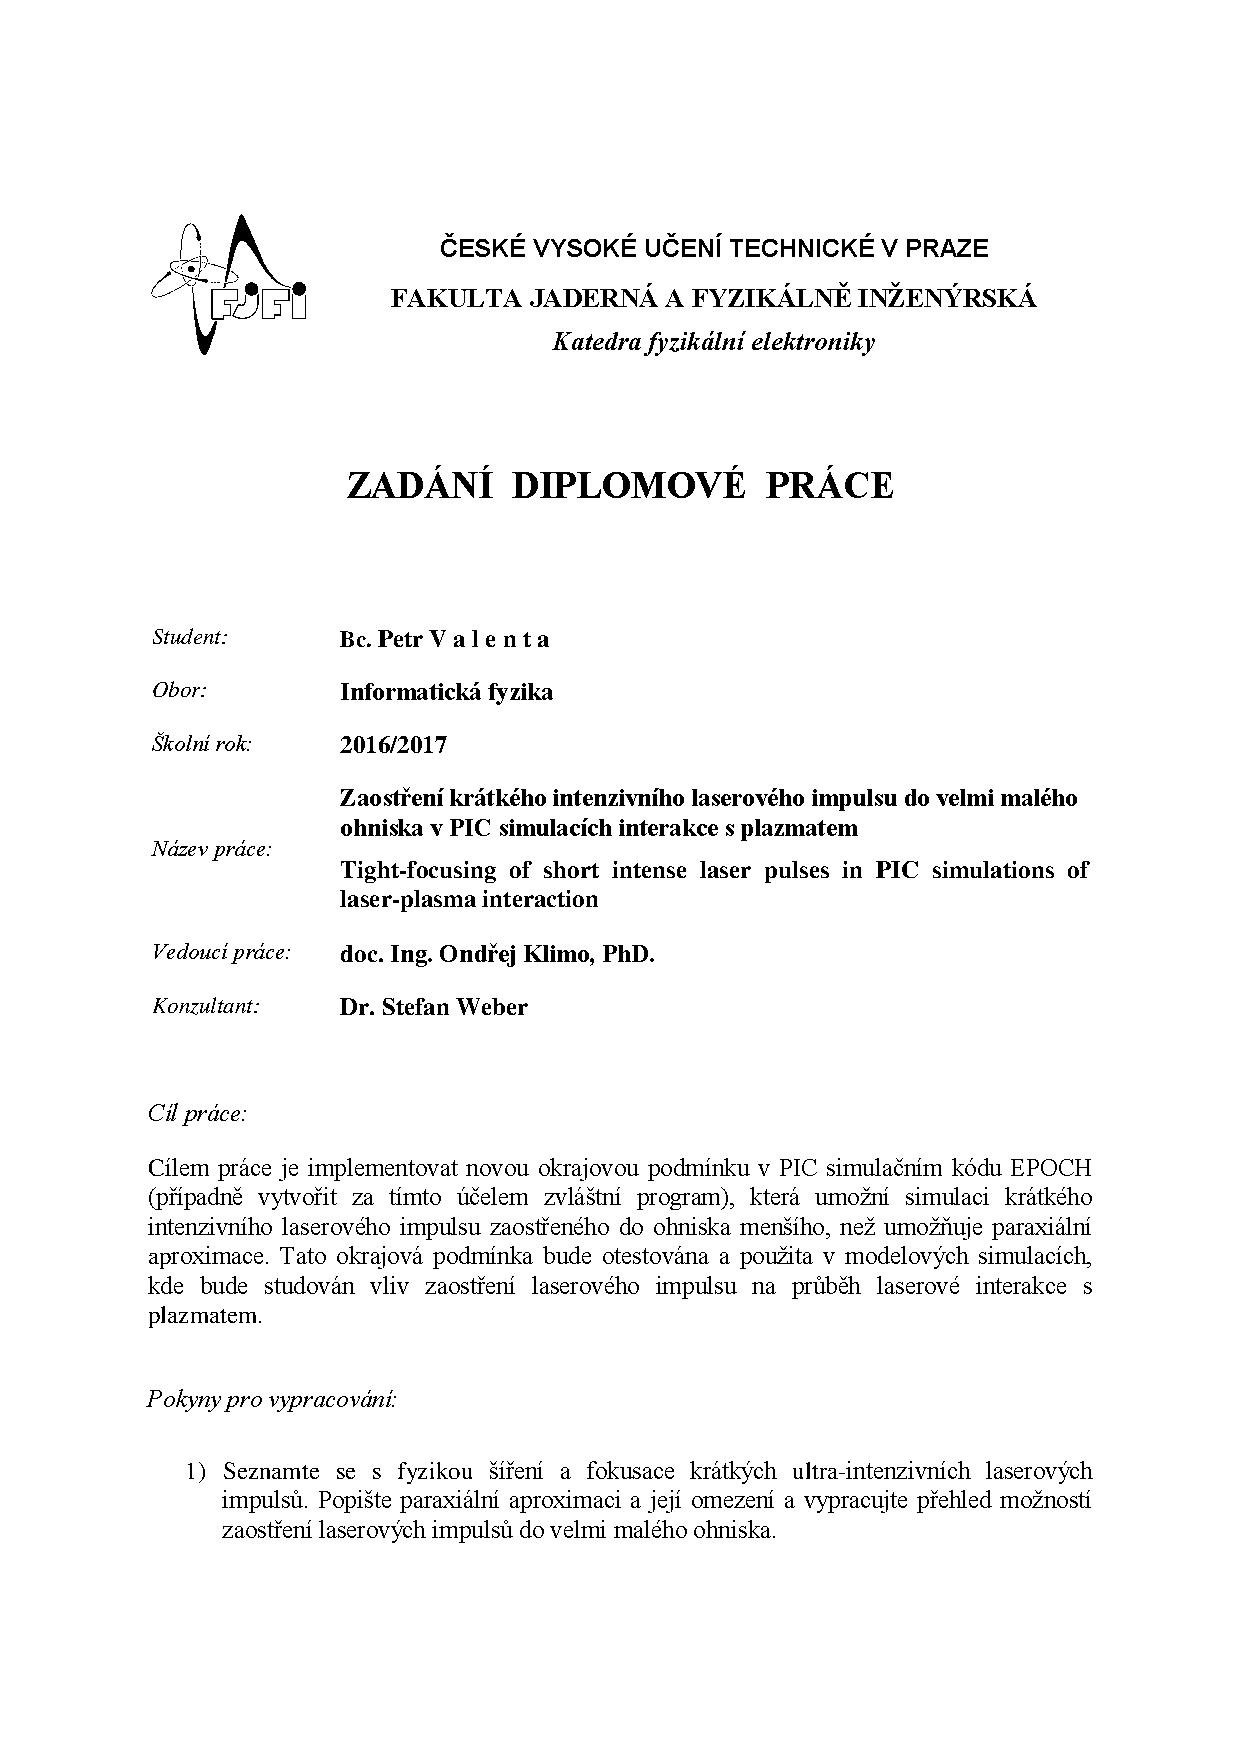
\includepdf[pages=1]{dat/zadani.pdf}

%4------------------------------------------------------------------------------

\newpage
\includepdf[pages=2]{dat/zadani.pdf}

%5------------------------------------------------------------------------------

\newpage
\null
\vfill
{\bf \noindent Prohlášení/Declaration} \\[5mm]
Prohlašuji, že jsem předloženou práci vypracoval samostatně a že jsem uvedl veškerou
použitou literaturu.\\[2mm]
I declare that I carried out this work independently, and only with the cited sources, literature and other professional sources.\\
\vspace{5mm}V Praze dne/In Prague on .............................\hfill
\begin{tabular}{c}
........................................\\
\valenta
\end{tabular}

%6------------------------------------------------------------------------------

\newpage
\thispagestyle{empty}
\mbox{}

%7------------------------------------------------------------------------------

\newpage
\begin{flushleft}
	\renewcommand{\arraystretch}{1.3}
	\begin{tabular}{r p{12cm}}
		Název práce:
		~ & \bf \projecttitlecz \\
		Autor:
		~ & \valenta \\
		Druh práce:
		~ & Diplomová práce \\
		Studijní program:
		~ & (N3913) Aplikace přírodních věd\\
		Vedoucí práce:
		Obor:
		~ & (3901T065) Informatická fyzika\\
		Vedoucí práce:
		~ & \klimo \newline Katedra fyzikální elektroniky, Fakulta jaderná a fyzikálně inženýrská, České vysoké učení technické v Praze \\
		Konzultant:
		~ & \weber \newline Projekt ELI-Beamlines, Fyzikální ústav Akademie věd České republiky, v. v. i. \\
	\end{tabular}
\end{flushleft}

\begin{center}
\textbf{Abstrakt}\\
\end{center}

Content...\\

Klíčová slova:


%8------------------------------------------------------------------------------

\newpage
\begin{flushleft}
	\renewcommand{\arraystretch}{1.3}
	\begin{tabular}{r p{12cm}}
		Title:
		~ & \bf \projecttitle \\
		Author:
		~ & \valenta \\
		Type of work:
		~ & Master thesis \\
		Study programme:
		~ & (N3913) Aplications of Natural Sciences	 \\
		Branch of study:
		~ & (3901T065) Computational Physics \\
		Supervisor:
		~ & \klimo \newline Department of Physical Electronics, Faculty of Nuclear Sciences and Physical Engineering, Czech Technical University in Prague \\
		Consultant:
		~ & \weber \newline Project ELI-Beamlines, Institute of Physics, The Czech Academy of Sciences, v. v. i. \\
	\end{tabular}
\end{flushleft}

\begin{center}
	\textbf{Abstract}\\
\end{center}

Content...\\

Keywords: plasma-based amplification, PIC simulations, parametric instabilities

%9------------------------------------------------------------------------------

\tableofcontents
\addtocontents{toc}{\protect\thispagestyle{empty}}
\thispagestyle{empty}

%-------------------------------------------------------------------------------

\pagestyle{myfancy}

\chapter*{Introduction\markboth{Introduction}{Introduction}}
\addcontentsline{toc}{chapter}{Introduction}
Since the first demonstration of pulsed laser in 1960 \cite{Maiman1960}, intense research and development in the field of laser technology have seen a tremendous progress. Pulse compression and amplification techniques, such as chirped-pulse amplification (CPA) \cite{StricklandMourou1985}, optical parametric chirped-pulse amplification (OPCPA) \cite{Dubietis1992} and lately backward Raman amplification (BRA) \cite{Malkin1999}, have enabled generation of ultra-short laser pulses with intensities exceeding $ 10^{21} \ \mathrm{W/cm^{2}} $ \cite{Danson2015}. Pulses in this regime provide an unprecedented capability for basic research (e.g. high-energy density physics, relativistic plasma physics and optics, laboratory astrophysics \cite{Council2003, Graziani2014, Lebedev2007, Bridgman1958, Krehl2008, Andreev2006, Weber2013, Bulanov2015, Zakharov2003}) as well as a broad range of groundbreaking applications in diverse fields (e.g. coherent diffractive imaging, X-ray diffraction and spectroscopy, pulse radiolysis, production of compact sources for radiotherapy \cite{Zewail2010, Bulanov2004, Malka2004}).

The peak laser intensities are typically amplified by increasing the input energy. This approach comes at great cost since it requires a higher level of complexity for the laser chain \cite{Fuchs2014}. A more effective route would be tight-focusing since the laser intensity is proportional to the square of the inverse of the focal spot size \cite{Kon2010}. In addition, focusing tightly may enhance the spatial and temporal contrast ratio of laser pulse which is crucial for many applications of laser-matter interaction \cite{Fuchs2014}. When using a conventional solid state optics, however, the laser beam diameter has to be increased in order to keep the energy density on the optical components below the damage threshold. Furthermore, additional care has to be taken to protect the optics from the target debris due to their short focal length \cite{Liu2011}. The solid state optics are thus inherently inappropriate in this case. Nevertheless, it seems that many drawbacks might be in future overcome by using a plasma-based focusing optics. Therefore, the tight-focusing and the interaction of tightly focused laser beams with matter are currently attracting much attention \cite{Popov2008, Popov2009, Lifschitz2016, Yan2005}. 

This work is structured as follows: the first chapter provides a brief introduction to the classical electromagnetic field theory, including the mathematical derivation of the paraxial Gaussian beam formula. The second chapter summarizes the elementary knowledge of plasma physics and physics of laser-plasma interaction. In the third chapter, one of the most popular numerical methods in plasma physics, particle-in-cell (PIC), is thoroughly discussed. The characteristics and features of the code EPOCH \cite{bennett}, which has been used for the simulations within this work, can be found in the last section of this chapter. The fourth chapter is devoted to the tight-focusing of laser pulses, including a description of algorithm for rigorous calculation of electromagnetic fields at boundaries of simulation domain \cite{Thiele2016}. This chapter also contains the details about the implementation of the algorithm as well as thorough evaluation of its correctness and the correctness of the implementation. At the end, one may find the overview of currently used experimental methods for tight-focusing. The last chapter demonstrates the results of several large-scale two-dimensional simulations employing tightly focused laser beams interacting with solid targets.

Although the convenient unit system for most plasma applications is the Gaussian cgs system, the SI (System Internationale) units are used throughout this work, unless explicitly stated. Symbols in bold represent vector quantities, and symbols in italics represent scalar quantities, unless otherwise indicated.


%-------------------------------------------------------------------------------

\chapter{Electromagnetic field}
The energy contained in an atomic nucleus can be obtained in two different ways. The first one consists in the splitting of heavy atomic nuclei into lighter elements. However, fission reaction entails some safety risks. In addition, the products of this reaction themselves are often unstable, and therefore give off relatively large amounts of radiation which cause some serious difficulties with their long term storage.

The second approach is nuclear fusion. It is the exact opposite process in which two or more atomic nuclei come very close and then join together to form a new type of atomic nucleus. If the mass of the product is less than the sum of the masses of the initial fusing nuclei, an amount of energy corresponding to this mass deficit is released in accordance with Einstein's famous relation. This chapter provides a brief insight into the challenges of nuclear fusion, particularly to one of the main approaches to achieve it - inertial confinement fusion.

\section{Maxwell's equations}
The electromagnetic field is in theory \cite{Stratton2007, Jackson2005, Feynman1963, Thide2011} represented by two vector quantities, the electric field intensity $ \vec{E}\left( \vec{r}, t \right) $ and the magnetic induction $ \vec{B}\left( \vec{r}, t \right) $. These vectors are finite and continuous functions of position $ \vec{r} $ and time $ t $. The description of electromagnetic phenomena in classical electrodynamics is provided by the set of Maxwell's equations. The microscopic variant with external sources in vacuum is formulated as follows \cite{Stratton2007},
\begin{equation}
\label{1.1}
\div{\vec{E}} = \frac{\rho}{\varepsilon_0},
\end{equation}
\begin{equation}
\label{1.2}
\div{\vec{B}} = 0,
\end{equation}
\begin{equation}
\label{1.3}
\rot{\vec{E}} + \diffp{\vec{B}}{t} = 0,
\end{equation}
\begin{equation}
\label{1.4}
\rot{\vec{B}} - \mu_0 \varepsilon_0 \diffp{\vec{E}}{t}= \mu_0 \vec{J},
\end{equation}
where $ \rho\left( \vec{r}, t \right) $ is total electric charge density and $ \vec{J}\left( \vec{r}, t \right) $ is total electric current density due to the motion of charged particles. These quantities may be continuous as well as discrete. As might be seen from the Maxwell's equations (\ref{1.1} - \ref{1.4}), the charge density is the source of the electric field, whilst the magnetic field is produced by the current density. The lack of symmetry in the equations (\ref{1.2}, \ref{1.3} are homogeneous) is caused by the experimental absence of magnetic charges and currents \cite{Thide2011}. The universal constants appearing in the Maxwell's equations (\ref{1.1}, \ref{1.4}) are the electric permittivity of vacuum $ \varepsilon_0 $ and the magnetic permeability of vacuum $ \mu_0 $.

The first equation, \ref{1.1}, is Gauss's law for electric field in the differential form. It states that the flux of the electric field through any closed surface is proportional to the total charge inside. The second equation, \ref{1.2}, is Gauss's law for magnetic field. It expresses the fact that there are no magnetic monopoles, so the flux of magnetic field through any closed surface is always zero. The third equation, \ref{1.3}, is Faraday's law describing how the electric field is associated with a time varying magnetic field. And the last equation, \ref{1.4}, is Amp\`ere's law with Maxwell's displacement current, which means that the time varying electric field causes the magnetic field. As a consequence, it predicts the existence of electromagnetic waves that can carry energy and momentum even in a free space.

To describe the effects of an electromagnetic field in the presence of macroscopic substances, the complicated distribution of charges and currents in matter over the atomic scale is not relevant \cite{Jackson2005}. Thus one shall define a second set of auxiliary vectors that represent fields in which the material properties are already included in an average sense, the electric displacement $ \vec{D}\left( \vec{r}, t \right) $ and the magnetic vector $ \vec{H}\left( \vec{r}, t \right) $ \cite{Feynman1963},
\begin{equation}
\label{1.5}
\vec{D} = \varepsilon_0 \vec{E} + \vec{P} = \varepsilon \vec{E},
\end{equation}
\begin{equation}
\label{1.6}
\vec{H} = \frac{\vec{B}}{\mu_0} - \vec{M} = \frac{\vec{B}}{\mu},
\end{equation}
where $ \vec{P}\left( \vec{r}, t \right) $ and $ \vec{M}\left( \vec{r}, t \right) $ are the vectors of polarization and magnetization, respectively. Note that the vectors of polarization and magnetization can be interpreted as a density of electric or magnetic dipole moment of the medium, therefore they are definitely associated with the state of a matter and vanish in vacuum \cite{Stratton2007}. Similarly as in the case of free space, the factors $ \varepsilon $ and $ \mu $ are called electric permittivity of medium and magnetic permeability of medium. In general case, $ \varepsilon $ and $ \mu $ are tensors. The constitutive relations above (\ref{1.5}, \ref{1.6}) hold only if the medium is homogeneous and isotropic \cite{Thide2011}. For the sake of simplicity, only such materials will be considered in the following text. The macroscopic variant of Maxwell's equations is formulated as follows \cite{Stratton2007},
\begin{equation}
\label{1.7}
\div{\vec{D}} = \rho,
\end{equation}
\begin{equation}
\label{1.8}
\div{\vec{B}} = 0,
\end{equation}
\begin{equation}
\label{1.9}
\rot{\vec{E}} + \diffp{\vec{B}}{t} = 0,
\end{equation}
\begin{equation}
\label{1.10}
\rot{\vec{H}} - \diffp{\vec{D}}{t} = \vec{J},
\end{equation}
where $ \rho\left(\vec{r}, t \right) $ and $ \vec{J}\left(\vec{r}, t \right) $ now stand for only external electric charge and current density, respectively.

By combining the time derivative of the equation \ref{1.7} with the divergence of the equation \ref{1.10}, one obtains the following relation between the electromagnetic field sources,
\begin{equation}
\label{1.11}
\diffp{\rho}{t} + \div{\vec{J}} = 0.
\end{equation}
The important result \ref{1.11}, which is frequently referred to as the equation of continuity, expresses nothing but the conservation of total electric charge in an isolated system \cite{Feynman1963}. In other words, the time rate of change of the electric charge in any closed surface is balanced by the electric current flowing through the surface.

\section{Electrodynamic potentials}
The first-order partial differential Maxwell's equations can be effectively converted to a smaller number of second-order equations by introducing electrodynamic potentials. Hence, one can express the electric and magnetic field as follows,
\begin{equation}
\label{1.12}
\vec{E} = -\grad{\Phi} - \diffp{\vec{A}}{t},
\end{equation}
\begin{equation}
\label{1.13}
\vec{B} = \rot{\vec{A}},
\end{equation}
where $ \Phi\left(\vec{r}, t \right) $ is the scalar potential and $ \vec{A}\left(\vec{r}, t \right) $ is the vector potential of the corresponding fields. One can clearly see that using the definitions \ref{1.12}, \ref{1.13}, six vector components are replaced by only four potential functions and two Maxwell's homogeneous equations (\ref{1.8}, \ref{1.9}) are fulfilled identically. 

However, by definitions \ref{1.12}, \ref{1.13}, $ \Phi\left(\vec{r}, t \right) $ and $ \vec{A}\left(\vec{r}, t \right) $ are not defined uniquely, thus an infinite number of potentials which lead to the same fields may be constructed. To avoid that, one has to impose a supplementary condition, for example
\begin{equation}
\label{1.14}
\div{\vec{A}} + \mu \varepsilon \diffp{\Phi}{t} = 0.
\end{equation}
The condition \ref{1.14} is called the Lorenz gauge. Lorenz gauge is commonly used in electromagnetism because of its independence of the coordinate system. Furthermore, it leads to the following uncoupled equations,
\begin{equation}
\label{1.15}
\laplace{\Phi} - \mu \varepsilon \diffp[2]{\Phi}{t} = -\frac{\rho}{\varepsilon},
\end{equation}
\begin{equation}
\label{1.16}
\laplace{\vec{A}} - \mu \varepsilon \diffp[2]{\vec{A}}{t} = -\mu \vec{J},
\end{equation}
that are in all respects equivalent to the Maxwell's equations and in many situations much simpler to solve.

Equations \ref{1.15}, \ref{1.16} correspond to the inhomogeneous wave equations for scalar potential $ \Phi\left(\vec{r}, t \right) $ and vector potential $ \vec{A}\left(\vec{r}, t \right) $. Their general solutions are given by the following expressions,
\begin{equation}
\label{1.17}
\Phi\left(\vec{r}, t \right) = \frac{1}{4 \pi \varepsilon} \int \frac{\rho\left(\vec{r^{\: \prime}}, t^{\: \prime} \right)}{\norm{\vec{r} - \vec{r^{\: \prime}}}} \mathrm{d} V,
\end{equation}
\begin{equation}
\label{1.18}
\vec{A}\left(\vec{r}, t \right) = \frac{\mu}{4 \pi} \int \frac{\vec{J}\left(\vec{r^{\: \prime}}, t^{\: \prime} \right)}{\norm{\vec{r} - \vec{r^{\: \prime}}}} \mathrm{d} V,
\end{equation}
where $ \mathrm{d} V $ is a volume element and $ \norm{.} $ stands for the standard Euclidean norm. Note that the solutions \ref{1.17}, \ref{1.18} are dependent only on charge and current densities at position $ \vec{r^{\: \prime}} $ at so-called retarded time $ t^{\: \prime} = t - \sqrt{\mu \epsilon} \norm{\vec{r} - \vec{r^{\: \prime}}} $ which takes into account the finite velocity of the wave. In other words, the fields at the observation point $ \vec{r} $ at the time $ t $ are proportional to the sum of all the electromagnetic waves that leave the source elements at point $ \vec{r^{\: \prime}} $ at the retarded time $ t^{\: \prime} $.

\section{Hertz vectors}
There exists also other possibilities how to express the electromagnetic field. Under ordinary conditions, an arbitrary electromagnetic field may be defined in terms of a single vector function \cite{Essex1977}. This may be helpful for solving of many problems of classical electromagnetic theory, particularly the wave propagation.

First, let us introduce the electric Hertz vector $ {\vec{\Pi_e}}\left(\vec{r}, t \right) $ in terms of the scalar and vector potentials \cite{Stratton2007},
\begin{equation}
\label{1.19}
\Phi = - \div{\vec{\Pi_e}},
\end{equation}
\begin{equation}
\label{1.20}
\vec{A} = \mu \varepsilon \diffp{\vec{\Pi_e}}{t}.
\end{equation}

Note that the definitions \ref{1.19}, \ref{1.20} are consistent with the Lorenz gauge condition \ref{1.14}. In the absence of magnetization, it might be easily shown that $ \vec{J} = \partial{\vec{P}}/\partial{t} $ and the electric Hertz vector $ {\vec{\Pi_e}}\left(\vec{r}, t \right) $ is governed by an inhomogeneous wave equation
\begin{equation}
\label{1.21}
\laplace{\vec{\Pi_e}} - \mu \varepsilon \diffp[2]{\vec{\Pi_e}}{t} = -\frac{\vec{P}}{\varepsilon}.
\end{equation}

The equation \ref{1.21} is of the same type as the equations \ref{1.15}, \ref{1.16} and has therefore the familiar general solution 
\begin{equation}
\label{1.22}
\vec{\Pi_e}\left(\vec{r}, t \right) = \frac{1}{4 \pi \varepsilon} \int \frac{\vec{P}\left(\vec{r^{\: \prime}}, t^{\: \prime} \right)}{\norm{\vec{r} - \vec{r^{\: \prime}}}} \mathrm{d} V.
\end{equation}
As might be seen form \ref{1.22}, the fields derived from the electric Hertz vector $ {\vec{\Pi_e}}\left(\vec{r}, t \right) $ can be interpreted as being due to a density distribution of electric dipoles \cite{Essex1977}. Every solution of \ref{1.22} then uniquely determines the electromagnetic field through
\begin{equation}
\label{1.23}
\vec{E} = \grad{\left(\div{\vec{\Pi_e}}\right)} - \mu \epsilon \diffp[2]{\vec{\Pi_e}}{t},
\end{equation}
\begin{equation}
\label{1.24}
\vec{B} = \mu \varepsilon \left(\rot{\diffp{\vec{\Pi_e}}{t}}\right).
\end{equation}

Second, one may introduce the magnetic Hertz vector $ {\vec{\Pi_m}}\left(\vec{r}, t \right) $ in terms of the scalar and vector potentials by the following expressions \cite{Stratton2007},
\begin{equation}
\label{1.25}
\Phi = 0,
\end{equation}
\begin{equation}
\label{1.26}
\vec{A} = \rot{\vec{\Pi_m}}.
\end{equation}
In the absence of polarization, $ \vec{J} = \rot{\vec{M}} $ and the magnetic Hertz vector $ {\vec{\Pi_m}}\left(\vec{r}, t \right) $ defined by \ref{1.25} and \ref{1.26} fulfills an inhomogeneous wave equation
\begin{equation}
\label{1.27}
\laplace{\vec{\Pi_m}} - \mu \varepsilon \diffp[2]{\vec{\Pi_m}}{t} = -\mu \vec{M}.
\end{equation}
As for the previous cases, one may easily find the solution of \ref{1.27},
\begin{equation}
\label{1.28}
\vec{\Pi_m}\left(\vec{r}, t \right) = \frac{\mu}{4 \pi} \int \frac{\vec{M}\left(\vec{r^{\: \prime}}, t^{\: \prime} \right)}{\norm{\vec{r} - \vec{r^{\: \prime}}}} \mathrm{d} V,
\end{equation}
thus the fields derived from the magnetic Hertz vector $ {\vec{\Pi_m}}\left(\vec{r}, t \right) $ may be imagined to be due to a density distribution of magnetic dipoles \cite{Essex1977}. Again, every solution of \ref{1.28} uniquely determines the electromagnetic field via
\begin{equation}
\label{1.29}
\vec{E} = \rot{\diffp{\vec{\Pi_m}}{t}},
\end{equation}
\begin{equation}
\label{1.30}
\vec{B} = \rot{\left(\rot{\vec{\Pi_m}}\right)}.
\end{equation}

Note that the above derivations considered electric and magnetic Hertz vectors as a separate quantities. It is also possible, however, to introduce them together in the form of one six-vector \cite{Nisbet1955}.

\section{Energy and momentum}
To be able to describe the interaction of the electromagnetic field with matter, one has to know the energy distribution throughout the field as well as the momentum balance.

By scalar multiplications of \ref{1.9} by $ \vec{H}\left( \vec{r}, t \right) $, of \ref{1.10} by $ \vec{E}\left( \vec{r}, t \right) $, following subtraction of both obtained equations and using standard vector identities, one gets the expression 
\begin{equation}
\label{1.31}
\vec{E} \cdot \diffp{\vec{D}}{t} + \vec{H} \cdot \diffp{\vec{B}}{t} + \div{\left(\vec{E} \times \vec{H} \right)} = -\vec{E} \cdot \vec{J}.
\end{equation}
The equation \ref{1.31} can be rewritten in the form of conservation law,
\begin{equation}
\label{1.32}
\diffp{u}{t} + \div{\vec{S}} = - \vec{E} \cdot \vec{J},
\end{equation}
where
\begin{equation}
\label{1.33}
u = \frac{1}{2} \left(\vec{E} \cdot \vec{D} + \vec{H} \cdot \vec{B} \right), \quad \vec{S} = \vec{E} \times \vec{H}.
\end{equation}
The quantity $ u\left( \vec{r}, t \right) $ in \ref{1.33} describes the total energy density in the field and $ \vec{S}\left( \vec{r}, t \right) $ is so-called Poynting vector which represents, in the equation \ref{1.32}, the energy flow of the field per unit area. Note that the Poynting vector points in the same direction as the vector of the wave propagation.

The important statement \ref{1.32}, also referred to as the Poynting theorem, expresses the conservation of energy for the electromagnetic field. In other words, the time rate of change of the field energy within a certain region and the energy flowing out of that region is balanced by the conversion of the electromagnetic energy into mechanical or heat energy and vice-versa.

Besides energy, the electromagnetic wave can carry also momentum. To derive a balance of linear momentum, one has to know the way how charges and currents interact with the electromagnetic field. This is described by the Lorentz force which density $ \vec{f}_\mathrm{L} \left( \vec{r}, t \right) $ is given by the following expression,
\begin{equation}
\label{1.51}
\vec{f}_\mathrm{L} = \rho \vec{E} + \vec{J} \times \vec{B}.
\end{equation}
Thus the electric and magnetic fields can be regarded as a forces produced by distribution of charge and currents.

By replacing sources in \ref{1.51} using macroscopic Maxwell's equations \ref{1.7}, \ref{1.10}, one may express the density of Lorentz force $ \vec{f}_\mathrm{L} \left( \vec{r}, t \right) $ entirely in terms of fields,
\begin{equation}
\label{1.52}
\vec{f}_\mathrm{L} = \left(\div{\vec{D}} \right) \vec{E} + \left(\rot{\vec{H}} \right) \times \vec{B} - \diffp{\vec{D}}{t} \times \vec{B}.
\end{equation}
Note that the last term on the right hand side of \ref{1.52} can be rewritten using the Poynting vector $ \vec{S}\left( \vec{r}, t \right) $ derived above, 
\begin{equation}
\label{1.53}
\diffp{\vec{D}}{t} \times \vec{B} = \varepsilon \mu \diffp{\vec{S}}{t} + \vec{D} \times \left(\rot{\vec{E}} \right).
\end{equation}
By plugging \ref{1.53} into \ref{1.52} and employing basic vector calculus identities, one eventually gets the expression for the linear momentum balance in the form of conservation law,
\begin{equation}
\label{1.54}
\diffp{\vec{g}}{t} + \div{\mathbb{T}} = -\vec{f}_\mathrm{L},
\end{equation}
where
\begin{equation}
\label{1.55}
\vec{g} = \varepsilon \mu \vec{S}, \qquad T_{ij} = - E_i D_j - H_i B_j + \frac{1}{2} \left(E_j D_j + H_j B_j \right) \delta_{ij}.
\end{equation}
The quantity $ \vec{g}\left( \vec{r}, t \right) $ in \ref{1.54} may be interpreted as the density of linear electromagnetic momentum and $ \mathbb{T}\left( \vec{r}, t \right) $ is so-called Maxwell stress tensor which represents, in the equation \ref{1.54}, the momentum flow per unit area. The symbol $ \delta_{ij} $ in \ref{1.55} stands for the Kronecker delta.

The important statement \ref{1.54}, which expresses the conservation of momentum for electromagnetic field, may be used to calculate the electromagnetic forces that act on objects or particles within that field. Notice that the contribution of the electromagnetic field to energy and momentum is completely characterized by the fluxes of $ \vec{S}\left( \vec{r}, t \right) $ and $ \mathbb{T}\left( \vec{r}, t \right) $.




\section{Electromagnetic waves and Gaussian beam}
In this section, the simplest mathematical description of a focused laser beam based on approximations to the wave equation is deduced. Since in numerical codes it is a common practice to prescribe the laser beams by their propagation in free space, the set of the microscopic Maxwell's equations \ref{1.1} - \ref{1.4} will be exploited.

In the absence of external sources, it might be easily shown that the equations \ref{1.1} - \ref{1.4} may be alternatively formulated as an uncoupled homogeneous wave equations for electric field $ \vec{E}\left( \vec{r}, t \right) $ and magnetic field $ \vec{B}\left( \vec{r}, t \right) $,
\begin{equation}
\label{1.34}
\laplace{\vec{E}} - \frac{1}{c^{2}} \diffp[2]{\vec{E}}{t} = 0,
\end{equation}
\begin{equation}
\label{1.35}
\laplace{\vec{B}} - \frac{1}{c^{2}} \diffp[2]{\vec{B}}{t} = 0,
\end{equation}
where the universal constant $ c = 1/\sqrt{\mu_0 \varepsilon_0} $ is the speed of light in vacuum, which leads to the essential fact, that the electromagnetic waves propagate in vacuum with the velocity of light $ c $. However, the wave equations \ref{1.34}, \ref{1.35} do not provide all the information about the electric and magnetic field of the wave. There are further constraints due to Maxwell's equations restricting the orientation and proportional magnitudes of the fields. From the set \ref{1.1} - \ref{1.4}, it might be clearly seen that $ \vec{E}\left( \vec{r}, t \right) $ and $ \vec{B}\left( \vec{r}, t \right) $ must be mutually perpendicular to each other as well as to the direction of the wave propagation. 

Without any loss of generality, consider the laser beam as a monochromatic electromagnetic wave propagating toward the positive direction of the z-axis. In many standard references, the description of such a wave is given by the evolution of a single electric field component linearly polarized along the x-axis of the Cartesian coordinate system \cite{Siegman1986, Milonni1988, Yariv1989, Svelto2010, Galvez2006} (although the more proper way would be to use the vector potential \cite{Davis1979, Davis1981, Guenther1990, Salamin2006, Vaveliuk2007}), therefore one has to look for the solution of the equation \ref{1.34}. 

According to the previous assumptions, the solution is expected to be in the form of the following plane wave,
\begin{equation}
\label{1.36}
\vec{E}\left(\vec{r_\bot}, z, t \right)  = \Re \ E_0 \Psi \left(\vec{r_\bot}, z \right) \e^{\i \left(k_z z - \omega t \right)} \mathrm{\vec{\hat{e}_x}},
\end{equation}
where $ \vec{r_\bot} = (x, y)^{\mathrm{T}} $ is the vector of transverse Cartesian coordinates, symbol $ \Re $ stands for the real part of the complex quantity, $ E_0 $ is a constant amplitude, $ \Psi \left(\vec{r_\bot}, z \right) $ is the part of the wave function which is dependent only on the spatial coordinates, $ \omega $ denotes the angular frequency, $ k_z $ is the z-component of the wave vector $ \vec{k}\left(\omega \right) $, $ \mathrm{i} $ denotes the imaginary unit and $ \mathrm{\vec{\hat{e}_x}} $ is the unit vector pointing in the direction of the x-axis.

Direct substitution of expression \ref{1.36} into the equation \ref{1.34} yields the time-independent form of the scalar wave equation
\begin{equation}
\label{1.37}
\laplace{\Psi \left(\vec{r_\bot}, z \right)} + 2 \i k_z \diffp{\Psi \left(\vec{r_\bot}, z \right)}{z} = 0.
\end{equation}
The equation \ref{1.37} is called the Helmholtz equation. Note that it is sufficient to seek solutions to the equation \ref{1.37} since the wave \ref{1.36} is monochromatic.

It turned out, that the geometry of the focused laser beam can be expressed in terms of the laser wavelength $ \lambda $ and the following three parameters,
\begin{equation}
\label{1.38}
w_0, \qquad z_{\mathrm{R}} = \frac{k_z w_0^2}{2} = \frac{\pi w_0^2}{\lambda}, \qquad \Theta = \frac{w_0}{z_\mathrm{R}} = \frac{\lambda}{\pi w_0}.
\end{equation}
The parameter $ w_0 $ in \ref{1.38} is the beam waist, defined as a radius at which the laser intensity fall to $ 1/\e^2 $ of its axial value at the focal spot. The second parameter, $ z_\mathrm{R} $, is so-called Rayleigh range which is a distance in the longitudinal direction from the focal spot to the point where the beam radius is $ \sqrt{2} $ larger than the beam waist $ w_0 $. And the last parameter, $ \Theta $, is the divergence angle of the beam that represents the ratio of transverse and longitudinal extent.

Because of the symmetry about the longitudinal axis of the equation \ref{1.37}, the following calculations may be made simpler by introducing a dimensionless cylindrical coordinates that use the parameters \ref{1.38},
\begin{equation}
\label{1.39}
\rho = \frac{\norm{\vec{r_\bot}}}{w_0}, \qquad \zeta = \frac{z}{z_{\mathrm{R}}}.
\end{equation}
After performing a transformation of coordinates, the Helmholtz equation \ref{1.37} becomes 
\begin{equation}
\label{1.40}
\frac{1}{\rho} \diffp{}{\rho}\left(\rho \diffp{\Psi \left(\rho, \zeta \right)}{\rho} \right) + 4 \i \diffp{\Psi \left(\rho, \zeta \right)}{\zeta}  = - \Theta^2 \diffp[2]{\Psi \left(\rho, \zeta \right)}{\zeta}.
\end{equation}
In the following calculations, the beam divergence angle $ \Theta $ is assumed to be small ($ \Theta \ll 1 $), thus it can be used as an expansion parameter for $ \Psi $ and the solution of \ref{1.40} will always be consistent,
\begin{equation}
\label{1.41}
\Psi = \sum_{n = 0}^{+\infty} \Theta^{2n} \Psi_{2n}.
\end{equation}
Next, one shall insert \ref{1.41} into \ref{1.40} and collect the terms with the same power of $ \Theta $. Then the zeroth-order function $ \Psi_0 $ obeys the following equation,
\begin{equation}
\label{1.42}
\frac{1}{\rho} \diffp{}{\rho}\left(\rho \diffp{\Psi_0 \left(\rho, \zeta \right)}{\rho} \right) + 4 \i \diffp{\Psi_0\left(\rho, \zeta \right)}{\zeta} = 0.
\end{equation}

The equation \ref{1.42}, which is called the paraxial Helmholtz equation, is the starting point of traditional Gaussian beam theory. One can expect the solution of \ref{1.42} in the form of a Gaussian function with a width varying along the longitudinal direction, thus 
\begin{equation}
\label{1.43}
\Psi_0 \left(\rho, \zeta \right) = h\left(\zeta \right)\e^{-f\left(\zeta \right) \rho^2},
\end{equation}
where $ f\left(\zeta \right) $ and $ h\left(\zeta \right) $ are unknown complex functions that have to satisfy a condition $ f\left(0 \right) = h\left(0 \right) = 1 $. After plugging \ref{1.43} into \ref{1.42}, one gets the following equation,
\begin{equation}
\label{1.44}
-f\left(\zeta \right) h\left(\zeta \right) + \i \diff{h\left(\zeta \right)}{\zeta} + \rho^2 h\left(\zeta \right) \left(f\left(\zeta \right)^2 - \i \diff{f\left(\zeta \right)}{\zeta} \right) = 0.
\end{equation}
Since the equation \ref{1.44} has to hold for arbitrary value of $ \rho $, one may find two independent equations that are equivalent to \ref{1.44}
\begin{equation}
\label{1.45}
\frac{1}{f\left(\zeta \right)^2} \diff{f\left(\zeta \right)}{\zeta} + \i = 0, \qquad \frac{1}{f\left(\zeta \right) h\left(\zeta \right)} \diff{h\left(\zeta \right)}{\zeta} + \i = 0.
\end{equation}
It might be easily shown, that under specified conditions the solutions of equations \ref{1.45} have to be
\begin{equation}
\label{1.46}
h\left(\zeta \right) = f\left(\zeta \right), \qquad f\left(\zeta \right) = \frac{1}{\sqrt{1 + \zeta^2}} \e^{-\i \arctan{\zeta}},
\end{equation}
and therefore the complete expression for the zeroth-order wave function $ \Psi_0 \left(\rho, \zeta \right) $ is
\begin{equation}
\label{1.47}
\Psi_0 \left(\rho, \zeta \right) = \frac{1}{\sqrt{1 + \zeta^2}} \exp{\left[- \frac{\rho^2}{1 + \zeta^2} + \i \left(\frac{\rho^2 \zeta}{1 + \zeta^2} - \arctan{\zeta} \right) \right]}.
\end{equation}

In many situations, it is also useful to evaluate the expression \ref{1.47} in terms of Cartesian coordinates, in which the zeroth-order wave function $ \Psi_0 \left(\vec{r_\bot}, z \right) $ is
\begin{equation}
\label{1.48}
\Psi_0 \left(\vec{r_\bot}, z \right) = \frac{w_0}{w\left(z\right)} \exp{\left[- \frac{\vec{r_\bot}^2}{w\left(z \right)^2} + \i \left( k_z \frac{\vec{r_\bot}^2}{2 R\left(z \right)} - \varphi_\mathrm{G} \left( z\right) \right) \right]},
\end{equation}
where the parameters used to simplify the expression \ref{1.48} are defined as
\begin{equation}
\label{1.49}
w\left(z\right) = w_0 \sqrt{1 + \left(\frac{z}{z_\mathrm{R}}\right)^2}, \quad R\left(z \right) = z \left[1 + \left(\frac{z_\mathrm{R}}{z} \right)^2\right], \quad \varphi_\mathrm{G}\left(z\right) = \arctan{\left(\frac{z}{z_\mathrm{R}}\right)}.
\end{equation}
One shall discuss the physical meaning of the three parameters \ref{1.49}. The function $ w\left(z\right) $ represents the spot size parameter of the beam, that is the radius at which the laser intensity fall to $ 1/\e^2 $ of its axial value at any position $ z $ along the beam propagation. Note that the minimum of the spot size $ w(0) = w_0 $, consequently the focal spot is stationary and located at the origin of a Cartesian coordinate system. The second parameter, $ R\left(z \right) $ is known to be the radius of curvature of the beam's wavefront at any position $ z $ along the beam propagation. Note that $ \lim_{z \to 0^{\pm}} R(z) = \pm \infty $, therefore the beam behaves like a plane wave at focus as required. The last parameter, $ \varphi_\mathrm{G}\left(z\right) $, is the so-called Guoy phase of the beam at any position $ z $ along the beam propagation, which describes a phase shift in the wave as it passes through the focal spot.

Finally, by substituting \ref{1.48} for $ \Psi \left(\vec{r_\bot}, z \right) $ in \ref{1.36} and taking the real part of that complex quantity, one obtains the electric field of the so-called paraxial Gaussian beam,
\begin{equation}
\label{1.50}
\vec{E}\left(\vec{r_\bot}, z, t \right) = E_0 \frac{w_0}{w(z)} \exp\left(-\frac{\vec{r_\bot}^2}{w(z)^2}\right) \cos\left(\omega t - k_z \left(z + \frac{\vec{r_\bot}^2}{2 R(z)} \right) + \varphi_\mathrm{G}\left(z\right) \right) \mathrm{\vec{\hat{e}_x}}.
\end{equation}
Although the electric field \ref{1.50} describes the main features of the focused laser beam, it might be clearly seen that it does not satisfy Gauss's law (\ref{1.1}). The correct electric field cannot vary with the direction of its polarization or has to have at least two non-zero vector components. To fix that, one would have to solve the wave equation for the vector potential \ref{1.16} and afterwards exploit the solution to deduce all components of the electric and magnetic fields.   

In addition, since one assumed $ \Theta \ll 1 $, the solution \ref{1.50} is not accurate for strongly diverging beams. Since the divergence angle is inversely proportional to the beam waist, the previous condition yields $ w_0 \gg \lambda $. In other words, it means that \ref{1.50} is not valid for tightly focused laser beams and the need may arise for higher-order corrections. 

%-------------------------------------------------------------------------------

\chapter{Laser-plasma interaction}
When a high-power laser pulse is focused onto the surface of a solid target, a high density plasma layer is produced almost immediately. The whole region dominated by laser-plasma interactions, which is called corona, expands radially outwards at sonic velocities.

In the inertial fusion experiments, it is essential to deliver the laser energy into the capsule of fusion fuel as much as possible. However, the efficient transport of radiation within the target strongly depends on non-linear processes that take place during the propagation of the laser light in the coronal plasma. 

Therefore, laser-plasma interactions provide a key gateway to the study of. In this chapter, a brief introduction to this exciting field, which is rich both in physics and in applications, is provided. 

\section{Basic plasma parameters}
Plasma, one of the four fundamental states of matter, is a quasi-neutral gas of charged and neutral particles which exhibits collective behavior \cite{Chen1984}. It is necessary to better explain some terms used in this definition.

By collective behavior one means motion that depends not only on local conditions but on the state of the plasma in remote regions as well. As charged particles move around, they can generate local concentrations of positive or negative charge, which give rise to electric fields. Motion of charges also generates currents, and hence magnetic fields. These fields affect the motion of other charged particles far away \cite{Chen1984}. Thus, the plasma supports a wide range of possible motions.

Quasi-neutrality describes the apparent charge neutrality of a plasma over large volumes, while at smaller scales, there can be charge imbalance, which may give rise to local electric fields. This fact can be expressed mathematically as
\begin{equation}
\label{2.1.1}
\sum_{s} q_s n_s \approx 0,
\end{equation}
where $ q_s $ and $ n_s $ is, respectively, the charge and density of particles of species $ s $. The index of summation is taken over all the particle species of given system.

One of the most important parameters, which allows to predict the behavior of plasmas more accurately, is the degree of its ionization. For a gas containing only single atomic species in thermodynamic equilibrium, the ionization can be clearly recognized from the Saha-Langmuir equation, which can be written in the following form \cite{Saha1920, Saha1921, Langmuir1923, Fridman2008},
\begin{equation}
\label{2.1.2}
\frac{n_{k+1}}{n_k} = \frac{2}{n_e h^3}\left(2\pi m_e k_B T\right)^{\frac{3}{2}} \frac{g_{k+1}}{g_k} \exp\left(-\frac{\varepsilon_{k+1} - \varepsilon_{k}}{k_{B} T} \right).
\end{equation}
Here $ n_k $ is the density of atoms in the k-th state of ionization, $ n_e $ is the electron density, $ m_e $ stands for the mass of electron, $ k_B $ is Boltzmann's constant, $ T $ is the gas temperature, $ h $ is Planck's constant, $ g_k $ is the degeneracy of the energy level for ions in the k-th state and $ \varepsilon_k $ is the ionization energy of the k-th level. From the equation (\ref{2.1.2}), it may be clearly seen that the fully ionized plasmas exist only at high temperatures. This is the main reason why plasmas do not occur naturally on Earth (with a few exceptions).

A fundamental characteristics of the plasma behavior is its ability to shield out the electric potentials that are applied to it. Therefore, another important quantity $ \lambda_{Ds} $, which is called the Debye length of species $ s $, is defined as \cite{Chen1984},
\begin{equation}
\label{2.1.3}
\lambda_{Ds} = \sqrt{\frac{\varepsilon_0 k_B T_s}{q_s^2 \, n_s}}.
\end{equation}
The physical constant $ T_s $ denotes the temperature of the particles of species $ s $. It often happens that a different species of particles in plasma have separate distributions with different temperatures, although each species can be in its own thermal equilibrium. The Debye length is a measure of the shielding distance or thickness of the sheath.

In plasma, each particle tries to gather its own shielding cloud. The previously mentioned concept of Debye shielding is valid only if there are enough particles in that cloud. Therefore, another important dimensionless number $ N_{Ds} $, which is called plasma parameter of species $ s $, is established. This parameter is defined as the average number of particles of species $ s $ in a plasma contained within a sphere of radius equal to the Debye length, thus \cite{Chen1984}
\begin{equation}
\label{2.1.4}
N_{Ds} = \frac{4}{3} \pi n_s \lambda_{Ds}^3. 
\end{equation}

Charge separation in plasma results in a typical harmonic electrostatic oscillations of charged particles described by the plasma frequency. One may define the plasma frequency for particles of species s \cite{Chen1984},
\begin{equation}
\label{2.1.5}
\omega_{ps} = \sqrt{\frac{q_s^{2}\,n_s}{\varepsilon_0 m_s}},
\end{equation}
Note that as the ions are much heavier than electrons, they do not respond to the high frequency oscillations of the laser electric field. In many of the phenomena described in this chapter, the ions are treated as an immobile, uniform, neutralizing background. However, if the frequency of external radiation source or the waves induced in plasmas is close to the ion plasma frequency, the ion motion must also be included. An example may be a stimulated Brillouin scattering \cite{kruer}.

A typical charged particle in plasma simultaneously undergoes Coulomb collisions with all the other particles in the Debye sphere. The importance of collisions is described by the collision frequency $ \nu_c $, which is the inverse of the mean time that it takes for a particle to significantly change its momentum due to collisions. The electron-ion collision frequency $ \nu_{ei} $ is given by the following relation \cite{nicholson},
\begin{equation}
\label{2.1.6}
\nu_{ei} = \frac{Z e^4 n_e}{4 \pi \varepsilon_0^2 m_e^2 v^3} \ln{\left(\Lambda\right)}, \qquad \Lambda = \frac{\lambda_D}{b_0}.
\end{equation}
The coefficient $ Z $ denotes the charge number, $ e $ is elementary charge, $ v $ is relative velocity of colliding particles and $ \ln{\left(\Lambda\right)} $ is the so-called Coulomb logarithm. It is ratio of the Debye to Landau length. Landau length $ b_0 $ is the impact parameter at which the scattering angle in the center of mass frame is $ 90^\circ $. For many plasmas of interest Coulomb logarithm takes on values between $ 5 - 15 $. In plasma, a single Coulomb collision rarely results in a large deflection. The cumulative effect of the many random small angle collisions, however, is often larger than the effect of the few large angle collisions \cite{Chen1984}. Notice that the collision frequency $ \nu_{ei} $ is proportional to $ v^{-3} $, therefore the effect of collisions in hot plasmas is usually weak.

In a constant and uniform magnetic field, one can find that a charged particle spirals in a helix about the magnetic field line. This helix defines a fundamental time unit and distance scale \cite{Chen1984},
\begin{equation}
\label{2.1.7}
\omega_{cs} = \frac{\abs{q_{s}} \norm{\vec{B}}}{m_{s}}, \qquad r_{Ls} = \frac{v_\perp}{\omega_{cs}}.
\end{equation}
These are called the cyclotron frequency $ \omega_{cs} $ and the Larmor radius $ r_{Ls} $ of species $ s $. Here $ v_\perp $ is a positive constant denoting the speed in the plane perpendicular to $ \vec{B} $.


\section{Plasma description}
There exist three different approaches to plasma physics. The particle theory, the kinetic theory and the hydrodynamic theory. Each approach has some advantages and limitations that stem from the simplified assumptions appropriate only for certain phenomena and time scales. Note that the coupling with the Maxwell's equations is usually straightforward, therefore the corresponding relations are not mentioned here. In the following three subsections, all the approaches are briefly discussed. 

%\subsection{Particle theory}
The time evolution of the system containing charged particles in plasma is influenced by the electromagnetic fields formed due to the motion of particles as well as the external fields (e.g. laser). The particle approach is based on solving the equations of motion for all the particles in the system. In this case, the motion of particles is governed by the Newton's equations with the Lorentz force,
\begin{equation}
\label{2.2.5}
m_s \diff[2]{\vec{r}}{t} = q_s \left(\vec{E} + \vec{v} \times \vec{B} \, \right).
\end{equation}
Note that the equation \ref{2.2.5} holds only for non-relativistic particles.

The particle theory is useful for tracking a single particle motion in prescribed electromagnetic field. Obviously, the general solution for the system of charged particles using this approach can be complicated since the plasma typically consist of a large number of such particles interacting with the self-consistent field. However, the full analysis for certain cases may be applied with the help of computing infrastructures and particle simulation codes.

%\subsection{Kinetic theory}
The plasma kinetic theory takes into account the motion of all charged particles in the system as well. However, the evolution of such system is not described by the exact motion of the particles, but only via certain average properties. The kinetic theory is based on a set of equations for the distribution function $ f_s \left(\vec{x}, \vec{v}, t \right) $ of particles of species $ s $ in plasma. The distribution function may be interpreted as a statistical description of a large number of interacting particles in the system \cite{nicholson}. If collisions can be neglected (for example in hot plasmas), the distribution function is governed by the collisionless Vlasov equation,
\begin{equation}
\label{2.2.1}
\diffp[]{f_{s}}{t} + \vec{v} \cdot \nabla f_s + \frac{q_{s}}{m_{s}}\left( \vec{E} + \vec{v} \times \vec{B} \right) \cdot \diffp[]{f_s}{\vec{v}} = 0.
\end{equation}
The Vlasov equation \ref{2.2.1} is obtained only by making the assumption that the particle density is conserved in the phase space, such that the time rate of change in a phase-space volume is equal to the flux of particles in or out of that volume \cite{nicholson}. Due to its simplicity, the equation \ref{2.2.1} is probably the most commonly used equation in the kinetic theory. However, the assumption to neglect collisions in a plasma is not valid generally. If it is necessary to take them into account, the collision term can be approximated using several methods \cite{Smirnov2008, nicholson, Chen1984, Drake2006, Boyd2003}.
 
%\subsection{Hydrodynamic theory}
In spite of the fact that the hydrodynamic theory is the roughest approximation for the description of plasma, it is sufficiently accurate to describe the majority of observed phenomena. The velocity distribution of each species is assumed to be Maxwellian everywhere, so the dependent variables are functions of only space and time coordinates \cite{Chen1984}. In other words, the fluid equations are the first three moments of the Vlasov equation (\ref{2.2.1}). These yield the following hydrodynamic equations for the density, momentum and the energy,
\begin{equation}
\label{2.2.2}
\diffp{n_s}{t} + \nabla \cdot \left(n_s \vec{u}_s \right) = 0,
\end{equation}
\begin{equation}
\label{2.2.3}
m_s n_s \left[ \diffp{\vec{u}_s}{t} + \left(\vec{u}_s \cdot \nabla \right) \vec{u}_s \right] + \nabla \cdot \mathbb{P}_s = q_s n_s \left(\vec{E} + \vec{u}_s \times \vec{B} \, \right),
\end{equation}
\begin{equation}
\label{2.2.4}
\diffp{}{t} \left(\frac{1}{2} n_s m_s u_s^2 + e_{s} \right) + \nabla \cdot \left(\frac{1}{2} n_s m_s u_s^2 \vec{u}_s + e_{s} \vec{u}_s + \mathbb{P}_s \vec{u}_s + \vec{Q}_s \right) = q_s n_s \vec{u}_s \cdot \vec{E}.
\end{equation}
The zeroth-order moment (\ref{2.2.2}) yields the continuity equation, where $ \vec{u}_s\left(\vec{x}, t \right) $ is the velocity of the fluid of species $ s $. This equation essentially states that the total number of particles is conserved. The first-order moment (\ref{2.2.3}) leads to a momentum equation. Here $ \mathbb{P}_s\left(\vec{x}, t \right) $ is the pressure tensor. This comes about by separating the particle velocity into the fluid and a thermal component of velocity. The thermal velocity then leads to the pressure term. Finally, the second-order moment (\ref{2.2.4}) corresponds to the energy equation, where $ e_{s} $ is the density of the internal energy and $ \vec{Q}_s $ describes the heat flux density.

It might be clearly seen that the moment equations do not form a closed system. For the system of equations \ref{2.2.2} - \ref{2.2.4} to be complete, it has to be supplemented by the equation of state, which describes the relation between pressure and density in the plasma. However, the equations of state are well defined only in local thermodynamic equilibrium. Otherwise, the system cannot provide sufficiently exact description and thus the fluid equations \ref{2.2.2} - \ref{2.2.4} are not appropriate. Note that if the magnetic field is dominant in plasma, the set of hydrodynamic equations \ref{2.2.2} - \ref{2.2.4} should be replaced by the equations of magnetohydrodynamics \cite{Boyd2003}.

\section{Electromagnetic waves in plasmas}
In laser-plasma interaction, the knowledge how the laser beam propagates through plasma is essential. Therefore, a general properties of the electromagnetic wave propagation in plasmas are closer described in this section. One can find the characteristics of propagation in both, unmagnetized as well as magnetized plasma. Particularly, in the case of magnetized plasmas, the waves traveling parallel to and perpendicular to a constant magnetic field are discussed in greater detail.

\subsection{Unmagnetized plasmas}
To derive the dispersion relation of electromagnetic wave propagating through unmagnetized plasmas, the hydrodynamic approach is exploited. Since one assume plasma response to a high frequency field, the ions are treated as a stationary, neutralizing background. Thermal motion of particles is also ignored, thus the pressure term in \ref{2.2.3} can be neglected. According to the previous assumptions, one shall solve the following set of equations,
\begin{equation}
\label{2.3.1.1}
\diffp{n_e}{t} + \nabla \cdot \left(n_e \vec{u}_e \right) = 0,
\end{equation}
\begin{equation}
\label{2.3.1.2}
m_e n_e \left[ \diffp{\vec{u}_e}{t} + \left(\vec{u}_e \cdot \nabla \right) \vec{u}_e \right] = - e n_e \vec{E}.
\end{equation}
One also needs the wave equation for the electric field \ref{1.34}. However, it is now necessary to include the current density due to motion of charged particles in plasma. The hydrodynamic equations are coupled with the Maxwell's equations via $ \vec{J} = q_s n_s \vec{u}_s $, thus the wave equation yields the following form,
\begin{equation}
\label{2.3.1.3}
\laplace{\vec{E}} - \frac{1}{c^{2}} \diffp[2]{\vec{E}}{t} = - \mu_0 e n_e \diffp{\vec{u}_e}{t},
\end{equation}

The system of equations above will be linearized using the methods of perturbation theory. Consider a small perturbations from the stationary state,
\begin{equation}
\label{2.3.1.4}
n_{e} = n_{e0} + \delta n_{e}, \quad \vec{u}_{e} = \vec{u}_{e0} + \delta \vec{u}_{e}, \quad \vec{E} = \vec{E}_{0} + \delta \vec{E},
\end{equation}
where $ \vec{u}_{e0} $ and $ \vec{E}_{0} $ are obviously identically equal to zero vector. After substituting perturbed quantities \ref{2.3.1.4} into initial system of equations and performing Fourier transform one obtains
\begin{equation}
\label{2.3.1.5}
\delta n_{e} = \mathrm{i} \frac{n_{e0}}{\omega} \vec{k} \cdot \delta \vec{u}_{e},
\end{equation}
\begin{equation}
\label{2.3.1.6}
\delta \vec{u}_e = -\i \frac{e}{\omega m_e} \delta \vec{E},
\end{equation}
\begin{equation}
\label{2.3.1.7}
\delta \vec{E} = \i \frac{\omega \, e \, n_{e0}}{\varepsilon_0 \left(\omega^2 - c^2 k^2 \right)} \delta \vec{u}_e.
\end{equation}
Note that the equation for density perturbation \ref{2.3.1.5} may be ignored. Eliminating $ \delta \vec{u}_{e} $ from the equation \ref{2.3.1.7} one gets the equation for perturbation of the electric field,
\begin{equation}
\label{2.3.1.8}
\left(\omega^2 - \omega_{pe}^2 - c^2 k^2 \right) \delta \vec{E} = 0. 
\end{equation}

The dispersion relation can be immediately obtained from the equation \ref{2.3.1.8}. To describe how the electromagnetic waves propagates through given medium, it is useful to introduce the index of refraction $ N \left( \omega \right) =  c k \left( \omega \right) / \omega $. Consequently, the dispersion relation may be rewritten as
\begin{equation}
\label{2.3.1.9}
N^{2} = 1 - \left(\frac{\omega_{pe}}{\omega}\right)^2.
\end{equation} 
The important properties of the waves are distinguished by their cut-offs ($ N \rightarrow 0 $) and resonances ($ N \rightarrow \infty $). In the vicinity of the resonance there is a total absorption, at a cut-off frequency there is a total reflection of incident waves.

In the case of the electromagnetic wave propagating through unmagnetized plasma, it might be clearly seen that there are no resonances. On the other hand, the equation \ref{2.3.1.9} exhibits cut-off and the corresponding frequency (including ions) is given by the following expression,
\begin{equation}
\label{2.3.1.10}
\omega = \sqrt{\omega_{pe}^{2} + \omega_{pi}^{2}}
\end{equation}
The condition \ref{2.3.1.10} occurs at the so-called critical plasma density $ n_c $. Note that the electromagnetic wave passing through plasma with densities larger than $ n_c $ is exponentially damped.

\subsection{Magnetized plasmas}
Next, consider the electromagnetic wave propagating through magnetized plasmas. To derive the dispersion relation, one may use similar treatment as in the previous subsection. The only difference is, that it is now necessary to include the effect of magnetic field. To obtain the wave equations for the oscillating electric and magnetic field, Faraday's law (\ref{1.3}) and Ampere's law (\ref{1.4}) are needed. The system of equations described above will be again linearized using a small perturbations from the stationary state,
\begin{equation}
\label{2.3.4}
\vec{u}_{e} = \vec{u}_{e0} + \delta \vec{u}_{e}, \quad \vec{B} = \vec{B}_{0} + \delta \vec{B}, \quad \vec{E} = \vec{E}_{0} + \delta \vec{E}.
\end{equation}
As in the previous case, $ \vec{u}_{e0} $ and $ \vec{E}_{0} $ are identically equal to zero vector. After substituting perturbed quantities (\ref{2.3.4}) into the initial system of equations and performing Fourier transform one obtains
\begin{equation}
\label{2.3.6}
\delta \vec{u}_{e} = - \mathrm{i} \frac{e}{m_{e} \omega} \delta \vec{E} - \mathrm{i} \frac{e}{m_{e} \omega} \delta \vec{u}_{e} \times \vec{B}_{0},
\end{equation}
\begin{equation}
\label{2.3.7}
\delta \vec{B} = \frac{1}{\omega} \vec{k} \times \delta \vec{E},
\end{equation}
\begin{equation}
\label{2.3.8}
\delta \vec{E} = - \frac{1}{\varepsilon_{0} \mu_{0} \omega} \vec{k} \times \delta \vec{B} + \mathrm{i} \frac{e n_{0}}{\varepsilon_{0} \omega} \delta \vec{u}_{e}.
\end{equation}

Eliminating $ \delta \vec{B} $ and $ \delta \vec{u}_{e} $ from the equation \ref{2.3.8} one gets the equation for perturbation of the electric field,
\begin{equation}
\begin{split}
\label{2.3.9}
& \left( \omega^{2} - \omega_{pe}^{2} - c^{2} k^{2} \right) \delta \vec{E} + \mathrm{i} \frac{\omega_{ce}}{\omega} \left( \omega^{2} - c^{2} k^{2} \right) \delta \vec{E} \times \vec{e}_{B} \: + \\[5pt]
& \qquad + c^{2} \left( \vec{k} \cdot \delta \vec{E} \right) \vec{k} + \mathrm{i} \frac{\omega_{ce}}{\omega} c^{2} \left( \vec{k} \cdot \delta \vec{E} \right) \vec{k} \times \hat{\vec{e}}_{B} = 0.
\end{split}
\end{equation}
Here $ \hat{\vec{e}}_{B} = \vec{B}_{0}/B_{0} $ is a unit vector in the direction of the magnetic field. If one choose, without the loss of generality, the coordinate system where $ \vec{B}_{0} = (0, 0, B_{0}) $ and $ \vec{k} = (k \sin \alpha, 0, k \cos \alpha) $, one obtains the equation $ \mathbb{M} \cdot \delta \vec{E} = 0 $ with the matrix
\begingroup
\renewcommand*{\arraystretch}{2.0}
\begin{equation}
\label{2.3.11}
\mathbb{M} =  \begin{pmatrix}
 \omega^{2} - \omega_{pe}^{2} - c^{2} k^{2} \cos^{2} \alpha & \mathrm{i} \dfrac{\omega_{ce}}{\omega} \left( \omega^{2} - c^{2} k^{2} \right)  & c^{2} k^{2} \cos \alpha \sin \alpha \\
 - \mathrm{i} \dfrac{\omega_{ce}}{\omega} \left( \omega^{2} - c^{2} k^{2} \cos^{2} \alpha \right) & \omega^{2} - \omega_{pe}^{2} - c^{2} k^{2} & - \mathrm{i} \dfrac{\omega_{ce}}{\omega} c^{2} k^{2} \cos \alpha \sin \alpha \\
 c^{2} k^{2} \cos \alpha \sin \alpha & 0 & \omega^{2} - \omega_{pe}^{2} - c^{2} k^{2} \sin^{2} \alpha
 \end{pmatrix}.
\end{equation} 
\endgroup
The system of equations has non-trivial solution if and only if $ \det \left( \mathbb{M} \right) = 0 $. This condition leads to the desired dispersion relation for an arbitrary angle $ \alpha $,
\begin{equation}
\begin{split}
\label{2.3.12}
& \ \ \left[ \left( \omega^{2} - \omega_{pe}^{2} - c^{2} k^{2} \cos^{2} \alpha \right) \left( \omega^{2} - \omega_{pe}^{2} - c^{2} k^{2} \alpha \right) - \left(  \frac{\omega_{ce}}{\omega} \right)^{2} \left( \omega^{2} - c^{2} k^{2} \right) \left( \omega^{2} - c^{2} k^{2} \cos^{2} \alpha \right) \right]\\[5pt]
& \left( \omega^{2} - \omega_{pe}^{2} - c^{2} k^{2} \sin^{2} \alpha \right) - c^{4} k^{4} \cos^{2} \alpha \sin^{2} \alpha \left[ \left( \omega^{2} - \omega_{pe}^{2} - c^{2} k^{2} \right) - \left( \frac{\omega_{ce}}{\omega} \right)^{2} \left( \omega^{2} - c^{2} k^{2} \right) \right] = 0.\\[5pt]
\end{split}
\end{equation}
\begingroup
\renewcommand*{\arraystretch}{2.4}
\begin{table}[t]
	\centering
	\begin{tabular}{ c | c | c }
		Wave & Cut-offs & Resonances \\ \hline \hline
		R & $ \omega_{R} = \dfrac{1}{2} \omega_{ce} + \dfrac{1}{2} \sqrt{\omega_{ce}^{2} + 4 \omega_{pe}^{2} } $ & $ \omega_{ce} = \dfrac{e B_{0}}{m_{e}} $ \\ \hline
		L & $ \omega_{L} = - \dfrac{1}{2} \omega_{ce} + \dfrac{1}{2} \sqrt{\omega_{ce}^{2} + 4 \omega_{pe}^{2}} $ & $ \omega_{ci} = \dfrac{Z e B_{0}}{m_{i}} $ \\ \hline
		O & $ \omega = \sqrt{\omega_{pe}^{2} + \omega_{pi}^{2}} $ & - \\ \hline
		X & $ \omega = \omega_{R}, \quad \omega = \omega_{L} $ & $ \omega_{lh} = \sqrt{\omega_{ce} \: \omega_{ci}}, \quad  \omega_{uh} = \sqrt{\omega_{pe}^{2} + \omega_{ce}^{2}}  $ \\
	\end{tabular}
	\caption{Summary of cut-offs and resonances for all the principal waves. Note that $ \omega_{lh} $ and $ \omega_{uh} $ are so-called lower hybrid frequency and upper hybrid frequency, respectively.}
	\label{table:1}
\end{table}
\endgroup
Now, it is necessary to find dispersion relations for the two simplest cases, propagation along and perpendicular to the magnetic field. For the waves propagating along $ \vec{B_{0}} $ $ \alpha = 0 $ and the dispersion relation \ref{2.3.12} gets relatively simple form,
\begin{equation}
\label{2.3.13}
\left( \omega^{2} - \omega_{pe}^{2} \right) \left[ \left( \omega^{2} - \omega_{pe}^{2} - c^{2} k^{2} \right)^{2}  - \left( \frac{\omega_{ce}}{\omega} \right)^{2} \left( \omega^{2} - c^{2} k^{2} \right)^{2} \right] = 0.
\end{equation}
The equation \ref{2.3.13} has three solutions. The first describes plasma oscillations at frequency $ \omega = \omega_{pe} $. The second and third solutions give right-handed (R) and left-handed (L) circularly polarized waves,
\begin{equation}
\label{2.3.14}
N_{R}^{2} = 1 - \frac{\left( \omega_{pe} / \omega\right)^{2} }{1 - \omega_{ce} / \omega}, \qquad N_{L}^{2} = 1 - \frac{\left( \omega_{pe} / \omega\right)^{2} }{1 + \omega_{ce} / \omega}.
\end{equation}
In a similar manner, for the waves propagating perpendicular to $ \vec{B_{0}} $ is $ \alpha = \pi/2 $ and the dispersion relation \ref{2.3.12} has the following form,
\begin{equation}
\label{2.3.15}
\left( \omega^{2} - \omega_{pe}^{2} - c^{2} k^{2} \right) \left[ \left( \omega^{2} - \omega_{pe}^{2} \right) \left( \omega^{2} - \omega_{pe}^{2} - c^{2} k^{2} \right) - \omega_{ce}^{2} \left( \omega^{2} - c^{2} k^{2} \right) \right] = 0.
\end{equation}
The equation \ref{2.3.15} has two solutions, which give ordinary (O) and extraordinary (X) waves,
\begin{equation}
N_{O}^{2} = 1 - \left( \frac{\omega_{pe}}{\omega} \right)^{2}, \qquad N_{X}^{2} = 1 - \left( \frac{\omega_{pe}}{\omega} \right)^{2} \frac{1 - \left( \omega_{pe} / \omega\right)^{2}}{1 - \left( \omega_{pe} / \omega\right)^{2} - \left( \omega_{ce} / \omega\right)^{2}}.
\end{equation}
The ordinary wave corresponds to a linearly polarized wave with electric field lying along the magnetic field direction, so that the motion remains unaffected. The extraordinary wave has the electric fields that are perpendicular to magnetic field, but with components both perpendicular and parallel to the wave vector. Note that all of the cut-offs and resonances of waves propagating through magnetized plasmas (including ions) are listed in the table \ref{table:1}.


\section{Ponderomotive force}
The ponderomotive force is probably the most important quantity that describes the interaction of high intensity laser pulses with plasma. It represents the gradient of the laser electric field that pushes charged particles in plasma into the regions of a lower field amplitude and it consequently leads to a wide range of non-linear phenomena that make the plasma inherently unstable. The ponderomotive force is involved e. g. in filamentation and self-focusing of laser beam, in the formation of cavities and solitons in the plasma profile or various parametric instabilities.

Note that since the mass of the ions is much higher than the electron mass, the ponderomotive force acting on ions is in most cases negligible. However, the ponderomotive force exerted on the electrons may be consequently transmitted to the ions by the electric field which is created due to the charge separation in plasma.

In the following two subsections, one can find the derivation of the ponderomotive force for the non-relativistic as well as the relativistic case. The derivation of the non-relativistic formula for ponderomotive force is easy to understand and clearly depicts its main characteristics that are valid even for the relativistic case. However, one has to be aware that the non-relativistic approximation breaks down if the laser intensity exceeds the values around $ 10^{18} \ \mathrm{W/cm^2} $. This may be the case of short or tightly focused laser beams. For this reason, the relativistic case is briefly discussed as well in the second subsection.

\subsection{Non-relativistic case}
The ponderomotive force can be derived from the motion of single particle in prescribed electromagnetic field. Thus one may exploit the Newton's equation of motion with the Lorentz force (\ref{2.2.5}). As the laser propagates through plasma, one may expect the oscillation of charged particles in a high-frequency electromagnetic field. For the mathematical description, one may exploit the so-called oscillation-center approximation in this case. It consist of splitting the radius vector $ \vec{r} $ and velocity $ \vec{v} $ of an arbitrary charged particle into two parts,
\begin{equation}
\label{2.5.1.2}
\vec{r} = \vec{r}_0 + \delta \vec{r}, \quad \vec{v} = \vec{v}_0 + \delta \vec{v},
\end{equation}
where the index $ 0 $ denotes the quantities at the center of oscillation and $ \delta \vec{x} = \vec{x} - \vec{x}_0 $ stands for the oscillating vector.

Next, one may exploit the Taylor series to  expand both, the electric field $ \vec{E}\left(\vec{r}, t\right) $ and magnetic field $ \vec{B}\left(\vec{r}, t\right) $ around the oscillation center $ \vec{r}_0 $,
\begin{equation}
\label{2.5.1.3}
\vec{E}\left(\vec{r}_0 + \delta \vec{r}, t\right) \cong \vec{E}\left(\vec{r}_0, t\right) + \left(\delta \vec{r} \cdot \nabla \right) \vec{E}\left(\vec{r}_0, t\right),
\end{equation}
\begin{equation}
\label{2.5.1.4}
\vec{B}\left(\vec{r}_0 + \delta \vec{r}, t\right) \cong \vec{B}\left(\vec{r}_0, t\right) + \left(\delta \vec{r} \cdot \nabla \right) \vec{B}\left(\vec{r}_0, t\right).
\end{equation}
Note that taking only the zeroth and first-order terms of the fields is sufficiently accurate approximation for the description of non-relativistic ponderomotive force.

By substituting \ref{2.5.1.2}, \ref{2.5.1.3} and \ref{2.5.1.4} into \ref{2.2.5} and collecting the terms of the same order, one obtains following two equations, 
\begin{equation}
\label{2.5.1.5}
m_s \diff[2]{\delta \vec{r}}{t} = q_s \left[ \vec{E}\left(\vec{r}_0, t\right) + \vec{v}_0 \times \vec{B}\left(\vec{r}_0, t\right)\right],
\end{equation}
\begin{equation}
\label{2.5.1.6}
m_s \diff[2]{\vec{r}_0}{t} = q_s \left[\left(\delta \vec{r} \cdot \nabla \right) \vec{E}\left(\vec{r}_0, t\right) + \delta \vec{v} \times \vec{B}\left(\vec{r}_0, t\right) \right]. 
\end{equation}

To solve equations \ref{2.5.1.5} and \ref{2.5.1.6}, assume further the laser fields in the form of standing monochromatic wave, 
\begin{equation}
\label{2.5.1.7}
\vec{E}\left(\vec{r}_0, t\right) = \vec{E}_0 \left(\vec{r}_0 \right) \cos \omega t, \quad  \vec{B}\left(\vec{r}_0, t\right) = - \frac{1}{\omega} \rot{\vec{E}_0 \left(\vec{r}_0 \right)} \sin \omega t.
\end{equation}
Note that the magnetic field in \ref{2.5.1.7} has been obtained by the integration of Faraday's law (\ref{1.3}). For the non-relativistic case, the term $ \vec{v}_0 \times \vec{B}\left(\vec{r}_0, t\right) $ is small in comparison with the term $ \vec{E}\left(\vec{r}_0, t\right) $ in the equation \ref{2.5.1.5}, thus it can be neglected. Taking into account the previous considerations, the solution of \ref{2.5.1.5} yields the oscillating quantities,
\begin{equation}
\label{2.5.1.8}
\delta \vec{r} = -\frac{q_s}{m_s \omega^2} \vec{E}_0 \left(\vec{r}_0 \right) \cos \omega t, \quad \delta \vec{v} = \frac{q_s}{m_s \omega} \vec{E}_0 \left(\vec{r}_0 \right) \sin \omega t.
\end{equation}
Since the integration constants can be considered as a slowly varying time functions, they have been included in $ \vec{r}_0 $.

By inserting \ref{2.5.1.8} into \ref{2.5.1.6} one gets immediately the following formula,
\begin{equation}
\label{2.5.1.9}
m_s \diff[2]{\vec{r}_0}{t} = - \frac{q_s^{2}}{m_s \omega^2} \left[\left(\vec{E}_0 \left(\vec{r}_0 \right) \cdot \nabla \right) \vec{E}_0 \left(\vec{r}_0 \right) \cos^2 \omega t + \vec{E}_0 \left(\vec{r}_0 \right) \times \left( \nabla \times \vec{E}_0 \left(\vec{r}_0 \right) \right) \sin^2 \omega t \right].
\end{equation}

To get the quasi-stationary ponderomotive force, one shall compute the time average values over the laser period $ T = 2 \pi/ \omega $. Thus by performing the time average of \ref{2.5.1.9} (note that $ \left\langle \sin^2 \omega t \right\rangle_T = \left\langle \cos^2 \omega t \right\rangle_T = 1/2$) one gets
\begin{equation}
\label{2.5.1.10}
m_s \left\langle \diff[2]{\vec{r}_0}{t} \right\rangle_{T} = - \frac{q_s^{2}}{2 m_s \omega^2} \left[\left(\vec{E}_0 \left(\vec{r}_0 \right) \cdot \nabla \right) \vec{E}_0 \left(\vec{r}_0 \right) + \vec{E}_0 \left(\vec{r}_0 \right) \times \left( \nabla \times \vec{E}_0 \left(\vec{r}_0 \right) \right)\right].
\end{equation}
The first term on the right-hand side of \ref{2.5.1.10} contributes to the transverse component of the ponderomotive force, whilst its longitudinal component originates from the second term. Utilizing standard identities of vector calculus, one finally gets the resulting quasi-stationary ponderomotive force $ \vec{F}_{\mathrm{p}} \left( \vec{r} \right) $ in the non-relativistic case,
\begin{equation}
\label{2.5.1.11}
\vec{F}_{\mathrm{p}} = - \grad{\Phi_{\mathrm{p}}}, \quad \Phi_{\mathrm{p}} = \frac{q_s^{2}}{4 m_s \omega^2} E_0^{2},
\end{equation}
where $ \Phi_{\mathrm{p}} \left( \vec{r} \right) $ is the corresponding ponderomotive potential, which may be interpreted as a cycle-averaged oscillation energy.

%Sometimes, it may be yet useful to have the expression for the ponderomotive force per unit volume $ \vec{f}_{p} \left( \vec{r} \right) $. To obtain it, one has to multiply the formula \ref{2.5.1.10} by the particle density. In the case of the electron fluid and normal laser light incidence on plasma, one gets the following easy-to-remember form,
%\begin{equation}
%\vec{f}_{p} = - \frac{\varepsilon_0}{4} \frac{\omega_{pe}^{2}}{\omega^{2}} \nabla E_0^{2}.
%\end{equation}

\subsection{Relativistic case}
The non-relativistic case is based on neglecting the term $ \vec{v} \times \vec{B} $ in the Newton's equation of motion (\ref{2.2.5}). However, this approximation is not valid for particles moving with velocities close to the velocity of light $ c $. The derivation of the relativistic ponderomotive force presented in this subsection follows [source].

A system containing a charged particle in an arbitrary electromagnetic field can be rigorously described using Lagrangian mechanics. The relativistic Lagrangian $ L \left( \vec{r}, \vec{v}, t \right)  $ for this case is given by the following expression,
\begin{equation}
\label{2.5.3.1}
L = -\frac{m_s c^2}{\gamma} - q_s \left(\Phi - \vec{v} \cdot \vec{A} \right), \quad \gamma = \left( 1 - \frac{v^{2}}{c} \right)^{-\frac{1}{2}}.
\end{equation}
For the traveling monochromatic wave, the Lagrangian $ L \left( \vec{r}, \vec{v}, t \right)  $ in \ref{2.5.3.1} can be transformed to $ L \left( \varphi \right)  $ using the wave phase $ \varphi = \vec{k} \cdot \vec{r} - \omega t $. The reason of doing this is that the transformed Lagrangian can be used to obtain the average over the wave period of motion,
\begin{equation}
\label{2.5.3.2}
\mathcal{L}_0 \left( \varphi \right) = \frac{1}{2 \pi} \int \limits_{\varphi}^{\varphi + 2\pi} \mathcal{L} \left( \varphi^{\: \prime} \right) \mathrm{d} \varphi^{\: \prime}, \quad \mathcal{L} \left( \varphi \right) = L \left( \varphi \right) \left( \diff{\varphi}{t} \right)^{-1}.
\end{equation}
Note that the Langrangian \ref{2.5.3.2} depends only on the quantities at the center of oscillation $ \vec{r}_0 $ and $ \vec{v}_0 $ defined through $ \varphi $. Then the motion of the oscillation center is governed by the Lagrange equations,
\begin{equation}
\label{2.5.3.3}
\diff{}{t} \left( \diffp[]{L_0}{\vec{v}_0} \right) -  \diffp[]{L_0}{\vec{r}_0} = 0, \quad L_0 \left( \varphi \right) = \mathcal{L}_0 \left( \varphi \right) \left( \diff{\varphi}{t} \right).
\end{equation}
The complete proof of assertions above can be found in [source].

The relativistic ponderomotive force in the oscillation center system can be easily found from the Lagrange equations \ref{2.5.3.3},
\begin{equation}
\vec{F}_{\mathrm{p}} \equiv \diff{}{t} \left( \diffp[]{L_0}{\vec{v}_0} \right) = -c^2 \grad{m_{\mathrm{eff}}},
\end{equation}
where the so-called effective mass $ m_{\mathrm{eff}} $ is the space and time dependent quantity that has been introduced as follows,
\begin{equation}
\label{2.5.3.4}
m_{\mathrm{eff}} = - \mathcal{L}_0 \frac{\gamma_0}{c^2} \left( \diff{\varphi}{t} \right), \quad  \gamma_0 = \left(1 - \frac{v_0^{2}}{c^{2}} \right)^{-\frac{1}{2}}.
\end{equation}
Note that the assertion \ref{2.5.3.4} holds for any electromagnetic field in vacuum in which it is possible to define the oscillation center. For ordinary conditions, the effective mass $ m_{\mathrm{eff}} $ can be rewritten as
\begin{equation}
m_{\mathrm{eff}} = m_s \sqrt{1 + \frac{q_s A^2}{\alpha m_s^2 c^2}}
\end{equation}
with $ \alpha = 1 $ for circular and $ \alpha = 2 $ for linear polarization of the electromagnetic wave. 

\section{Self-induced transparency (SIT)}
Plasma is strongly non-linear medium. This means that it may be accompanied by very strong electric fields and its non-linearities can be excited easily. When laser pulse with intensity above certain threshold irradiates the plasma, a number of collective non-linear processes may occur which can either enhance or reduce the energy absorption. As discussed before, the knowledge of the penetration depth and absorbed fraction of the incident energy is of vital importance for inertial confinement fusion research. 

The non-linear interaction is conveniently described in terms of light pressure and the ponderomotive force, which is introduced first. In the next section, the parametric instabilities are discussed as a consequence of non-linear coupling of electromagnetic laser waves to the plasma. The last section describes the laser beam filamentation and self-focusing.

\section{Laser absorption and electron heating mechanisms}
Absorption of laser energy during the laser-plasma interaction is an important issue to be investigated. The energy of laser pulses can be absorbed in plasma by various different non-linear mechanisms depending on the laser intensity. For the laser intensities considered within this work (above $ 10^{16} \ \mathrm{W/cm^2} $), the plasma is predominantly heated by collisionless absorption mechanisms. These mechanisms are generally characterized by the fact that the energy is transfered to a relatively small part of so-called hot electrons. In the following three subsections, the main mechanisms of collisionless plasma heating are briefly described.


\subsection{Resonance absorption}
The energy of laser beam may be absorbed by resonance absorption in the plasma. It is a linear process in which an incident laser wave is partially absorbed by conversion into an electron wave at the critical density of plasma $ n_c (\omega) $.

Resonance absorption takes place when a linearly p-polarized laser pulse is obliquely incident on a plasma with an inhomogeneous density profile. A component of the electric laser field perpendicular to the target surface then resonantly excites an electron plasma wave also along the plasma density gradient, thus a part of the laser wave energy is transferred into the electrostatic energy of the electron plasma wave \cite{eliezer}. This wave propagates into the underdense plasma and is damped either by collision or collisionless absorption mechanisms. Consequently, the energy is further converted into the thermal energy which heats the plasma and may possibly produce hot electrons.

Particularly, resonance absorption is the main absorption process for the laser beams of higher intensities and longer wavelengths. The efficiency of the resonance absorption may also be higher in plasma with high temperature, low critical density, or short scale length of the density profile.


\subsection{Brunel's vaccum heating}
Similarly as for the resonance absorption, Brunel's vaccum heating takes place when a linearly p-polarized laser pulse is obliquely incident on a plasma. In this case, however, the incident angle must be relatively large. Moreover, the plasma density profile has to be steep, so the amplitude of the oscillating electrons driven by the electric laser field is larger than the density scale length. Consequently, the energy of laser pulse carried by electrons is transfered into mechanical or heat energy in the overdense plasma region \cite{Gibbon2005}.

The energy absorbed via Brunel's vacuum heating is carried by hot electrons in the bunches
ejected once per laser period. To give a physical picture, in the first half of laser cycle, the electrons are pushed inside the plasma gaining only a small amount of energies because the electric laser field is shielded. On the other hand, in the second half of laser cycle, the electrons gain very high energies while they are ejected into vacuum. 

The trajectory of charged particles is strongly influenced by the time of their expulsion. Furthermore, a self-consistent electric field may be generated if a large amount of charged particles is ejected at the same time. The majority of the charged particles, however, returns into the plasma and propagates behind the skin layer where the laser electric field is screened so they can travel virtually unhindered into the target. Note that since the charged particles are accelerated by different phases of the laser field, the distribution of such particles can be in most cases considered as a Maxwellian \cite{Gibbon2005}.

\subsection{Relativistic $ \vec{J} \times \vec{B} $ heating}
For the relativistic laser beams, the high-frequency $ \vec{v} \times \vec{B} $ component of the Lorentz force becomes important and may contribute to plasma heating. Similarly to the Brunel's vacuum heating, discussed in the previous subsection, $ \vec{J} \times \vec{B} $ heating requires very steep plasma density gradients. On the contrary, this heating scenario works for any polarization apart from circular and is most efficient for the laser pulses normally incident onto the target surface, so there is no oscillating component of the electric field perpendicular to plasma \cite{Gibbon2005}.

In the case of $ \vec{J} \times \vec{B} $ heating, the absorbed energy is carried by bunches of hot electrons that are ejected twice per laser period \cite{Gibbon2005}. This fact may help to distinguish between the effects of Brunel's and $ \vec{J} \times \vec{B} $ heating. Again, the ejected electrons are pushed back into the plasma by self-consistent electric field generated by charged particles without restoring forces behind the skin layer.

\section{Mechanisms of laser-driven ion acceleration}
Because of the relatively large ion mass, currently achievable laser intensities are not strong enough to accelerate protons or heavier ions directly to sufficiently high energies. However, ions typically respond on slowly varying electric fields in plasma arising from the strong charge separations induced by various phenomena that take place during the interaction of intense laser beam with matter.

As one may see later, ions can be either accelerated in the vicinity of the laser focal spot at the front side of the target as well as in the vicinity of the target-vacuum boundary at the rear side. In the last two subsections of this chapter, the two main mechanisms for ion acceleration in laser-plasma interactions are briefly described.

\subsection{Radiation pressure acceleration (RPA)}
Radiation pressure acceleration (RPA) stands for the mechanism in which the ions are accelerated from the target front side in the vicinity of the laser focal spot. The acceleration is driven by the ponderomotive force (see the section 2.4) which expels the electrons into the regions of a lower laser intensities and consequently generates a strong electrostatic fields as a result of a charge separation. In the case of intense laser beams, the radiation pressure is strong enough to push an overdense target inwards whilst changing the shape of its surface and correspondingly the density profile. This process is commonly named hole boring.

For a plane, monochromatic wave at a normal incidence onto a target at rest, the balance between the electrostatic pressure and the radiation pressure at the target surface can be expressed as follows,
\begin{equation}
\label{2.7.1.1}
\frac{1}{2} \varepsilon_0 E_{\mathrm{es}}^2 = \frac{\left( 1 + R - T \right)}{c} I,
\end{equation}
where $ \vec{E}_{\mathrm{es}} \left(\vec{r}, t \right) $ is the electrostatic field generated by the charge separation, $ R $ and $ T $ are the reflection and transmission coefficients of the target, respectively, and $ I $ is the intensity of incident laser pulse.

The formula \ref{2.7.1.1} determines the extension of a charge depletion layer, which is established at the front side of the target. Ions in the depletion layer are accelerated by the electrostatic field $ \vec{E}_{\mathrm{es}} \left(\vec{r}, t \right) $, which amplitude can be obtained by solving the Poisson equation. The maximum energy, that the ions may gain, is then estimated as follows [source],
\begin{equation}
\mathcal{E}_{max} = \frac{Z m_e c^2 a_0^2}{m_i \gamma}, \quad \gamma = \sqrt{1 + \frac{a_0^2}{2}}.
\end{equation}
 
The RPA regime starts to dominate for a laser beams with peak intensity higher than $ 10^{21} \  \mathrm{W/cm}^2 $. Also, RPA could be more efficient for circularly polarized laser beams normally incident onto a target, because of their ability to suppress the effects of electron heating mechanisms mentioned in the previous section. Note that the RPA mechanism typically produce an ion beam of a large divergence because the critical density interface where the charge separation occurs is curved by the shape of the laser beam.



\subsection{Target normal sheath acceleration (TNSA)}
The interaction of intense laser beam with matter typically produce a population of hot electrons that may pass through the target and propagate beyond its rear side. This leads to generation of a strong electrostatic potential which accelerates the ionized particles in the direction normal to the target rear surface. Therefore, this mechanism is commonly known as target normal sheath acceleration (TNSA). TNSA can be also observed on the target front, because hot electrons are also expelled by the laser pulse into the vacuum on this side of the target.

The approximation for TNSA mechanism can be provided either by the static or dynamic model of the sheath. In the following, a dynamic model based on a free isothermal expansion of electron-ion plasma into vacuum is briefly described.

To find a non-linear solution that corresponds to the isothermal rarefaction wave, one may exploit the hydrodynamic equations for an ion component,
\begin{equation}
\label{2.7.2.2}
\diffp{n_i}{t} + \div{\left(n_i \vec{u}_i\right)} = 0,
\end{equation}
\begin{equation}
\label{2.7.2.3}
\diffp{\vec{u}_i}{t} + \left(\vec{u}_i \cdot \grad{} \right) \vec{u}_i = \frac{Z e}{m_i} \vec{E}. 
\end{equation}

Assume that at time $ t = 0 $, the electron density satisfies the Boltzmann distribution and the ion density occupies a half space with an infinitely sharp boundary, thus
\begin{equation}
\label{2.7.2.1}
n_e = n_{e0} \exp{\left( \frac{e \Phi}{k_B T_e} \right)}, \quad n_i = n_{i0} H(x).
\end{equation}
Assume further that the plasma is locally neutral on the scale length larger than the Debye radius, therefore $ n_e = Z n_i $. However, one shall be aware that the condition for the local neutrality does not imply that there is no electrostatic field. The electrostatic field may arise due to the sources coming from the regions where the condition for quasi-neutrality does not hold. Therefore, the electric field  $ \vec{E} \left(\vec{r}, t\right) $ in the equation \ref{2.7.2.3} may be replaced by the electrostatic field $ \vec{E}_{es} \left(\vec{r}, t\right) = -\grad{\Phi} \left(\vec{r}, t\right) $, which one can obtain by taking the gradient of the electron density \ref{2.7.2.1}. After replacing the electric field $ \vec{E} \left(\vec{r}, t\right) $ in the equation \ref{2.7.2.3} one gets
\begin{equation}
\label{2.7.2.5}
\diffp{\vec{u}_i}{t} + \left(\vec{u}_i \cdot \grad{} \right) \vec{u}_i = - \frac{c_s^2}{n_i} \grad{n_i}, \quad c_s = \sqrt{\frac{Z k_B T_e}{m_i}},
\end{equation}
where $ c_s \left(\vec{r}, t\right) $ is the ion-acoustic velocity. By performing the Fourier transforms of the equations \ref{2.7.2.2} and \ref{2.7.2.5}, one easily obtains the dispersion relation of the ion-acoustic waves. However, the system has also a non-linear self-similar solution which describes the rarefaction wave. Thus, define a self-similar variable in 1D geometry as $ \xi = x/t $. The ion fluid density and velocity then become $ n_i \left(x, t\right) = N \left( \xi \right) $ and $ u_i \left(x, t\right) = V \left( \xi \right) $, respectively. After transformation, the system of equations \ref{2.7.2.2} and \ref{2.7.2.5} yields
\begin{equation}
\label{2.7.2.6}
\frac{1}{N} \diff{N}{\xi} = - \frac{V - \xi}{c_s},
\end{equation}
\begin{equation}
\label{2.7.2.7}
\diff{V}{\xi} = - \frac{1}{N} \diff{N}{\xi} \left(V - \xi \right).
\end{equation}

Now, the set of equations \ref{2.7.2.6}, \ref{2.7.2.7} can be solved easily. The solution in the original coordinates can be found below,
\begin{equation}
\label{2.7.2.8}
n_i = n_{i0} \exp \left( -\frac{x}{c_s t} - 1 \right), \quad u_i = c_s + \frac{x}{t}.
\end{equation}
Note that the solution \ref{2.7.2.8} is valid only for $ x > -c_s t $ where $ u_i > 0 $. The condition $ x = - c_s t $ describes the rarefaction front propagating backwards into the target at the speed $ c_s $. Finally, by plugging the solution \ref{2.7.2.8} into the equation \ref{2.7.2.3}, one may find the expression for the electric field at the ion front $ x = - c_s t $,
\begin{equation}
\label{2.7.2.9}
E_x = \frac{2 E_0}{\omega_{pi} t}, \quad E_0 = c_s \sqrt{\frac{n_i m_i}{\varepsilon_0}}.
\end{equation}

The apparent drawback of formula \ref{2.7.2.9} is that it has a singularity at time $ t = 0 $. However, one may find a simple expression for the electric field at $ t = 0 $ by integration of the Poisson's equation from $ x = 0 $ to $ x = +\infty $,
\begin{equation}
\label{2.7.2.10}
E_x = \sqrt{\frac{2}{e}} E_0.
\end{equation}
A very precise interpolation of the electric field at the ion front, which is valid for any time, has been already found [source],
\begin{equation}
\label{2.7.2.11}
E_x \cong \frac{2 E_0}{\sqrt{2e + \omega_{pi}^2 t^2}}.
\end{equation}
As a consequence of formula \ref{2.7.2.11}, one may find relatively accurate prediction of the corresponding ion front velocity by solving the equation of motion \ref{2.7.2.3} with the electric field \ref{2.7.2.11},
\begin{equation}
\label{2.7.2.12}
u_i \cong 2 c_s \ln \left[ \frac{\omega_{pi} t}{\sqrt{2 e}} + \left(\frac{\omega_{pi}^2 t^2}{2 e} + 1 \right)^{\frac{1}{2}} \right].
\end{equation}
The maximum ion energy is then proportional to the temperature of hot electrons, which scales with the ponderomotive potential ($ \sim \sqrt{I \lambda^2} $) [source].

The next drawback of the model is that the derived formula for maximum velocity of ions \ref{2.7.2.12} diverges logarithmically with time, therefore the system accelerates the ions infinitely. This result comes from the isothermal assumption. Nevertheless, one might overcome this drawback by assuming the finite thickness of plasma or by introducing a maximum acceleration time constant at which the ion acceleration stops [source].

%-------------------------------------------------------------------------------

\chapter{Particle-in-cell (PIC)}
The collective behavior of particles and fields in laser-plasma interactions represent a complex and strongly non-linear problem. The investigation of such systems cannot be carried out only through the application of two traditional techniques, namely, theoretical and experimental work. Since there is a large number of a very complex simultaneous interactions with many degrees of freedom in plasma, analytical modeling seems to be impractical. On the other hand, many of the significant details of laser-plasma interaction are extremely difficult or even impossible to obtain experimentally. Therefore, for the further understanding in this field of research other tools and techniques are required \cite{jaroszynsky}.

Numerical simulation is now an integrated part of science and technology. With the advent of powerful computational systems, numerical simulations now play an important role in physics as an essential tool in developing theoretical models and understanding experimental results. Numerical simulation is now rightfully considered as a separate discipline from theory and experiment \cite{pang}.

Numerical simulations help researchers to develop models covering a wide range of physical scenarios and to investigate their properties. For example, numerical schemes for Newton's equation can be implemented in the study of the molecular dynamic, the techniques used to solve hydrodynamic equations are needed in weather prediction and algorithms for solving the diffusion equation can be applied to air pollution control problems. Only one numerical code can solve a variety of physical problems by modification of the initial and boundary conditions. These so-called computer experiments are often faster and much cheaper than a single real experiment in laboratory \cite{gould}.
 
Nowadays, it is clear that a detailed understanding of the physical mechanisms in laser-plasma interaction can only be achieved through the combination of theory, experiment and simulation. Development of parallel algorithms that lead to a stable and sufficiently exact solution, however, belong to the most challenging fields of modern science.

The most part of this chapter is focused on the description of the particle-in-cell method, which is the very popular numerical algorithm used for plasma simulations. There can be found the mathematical background of this method, description of the steps of the simulation loop and stability conditions. The last section provides a brief overview of the particle-in-cell code EPOCH, which has been used for simulations within this work.

\section{Mathematical derivation}
Laser-plasma interaction involves a collective behavior of particles and electromagnetic fields which is in general case complex and strongly non-linear problem to solve. The investigation of such systems cannot be usually carried out only through the theoretical and experimental work. Since a large amount of simultaneous interactions with many degrees of freedom may be present there, analytical modeling seems to be impractical. On the other hand, many of the significant details of laser-plasma interaction may be extremely difficult or even impossible to obtain experimentally. Hence, for the further progress in this field of research, other tools and techniques are required \cite{jaroszynsky}.

Numerical simulations help researchers to develop models covering a wide range of physical scenarios as well as to investigate their properties. With the advent of powerful computational systems, numerical simulations now play an important role as an essential tool in developing theoretical models and understanding experimental results in various fields of modern science \cite{pang}. These so-called computer experiments are often faster and much cheaper than a single real experiment in laboratory \cite{gould}. In addition, one numerical code can solve a broad range of tasks only by modification of its initial and boundary conditions.

Nowadays, it is clear that detailed understanding of the physical mechanisms in the laser-plasma interaction can be achieved only through the combination of theory, experiment and simulation. Development of parallel algorithms that are able to provide sufficiently exact solutions in reasonable time, however, belongs to the most challenging fields of modern science.

The PIC method refers to a technique that has been used to solve a certain class of partial differential equations. The method has been proposed in the mid-fifties and it has early gained a great popularity in the field of plasma physics. It is based on the kinetic description approach, thus the evolution of the system is conducted in principle via the motion of the charged particles.

However, real systems are often extremely large in terms of the number of particles they contain. In order to make simulations computationally tractable, so-called macro-particles are used. The macro-particle is a finite-size computational particle representing a group of physical particles that are near each other in the phase space. Notice that it is allowed to rescale the number of particles, because the Lorentz force depends only on the charge to mass ratio, which is invariant to this transformation. Thus, the macro-particle will follow the same trajectory as the corresponding real particles would \cite{hockney}.

Although this approach significantly reduces the number of computational particles in simulation, the binary interactions for every pair of a system cannot be taken into account. The cost would scales quadratically as the number of particles increases and that makes the computational effort unmanageable in the case of larger systems. Fortunately, many of the phenomena occur in high-temperature plasmas where the collective behavior dominates and the collisional effects are very weak (see \ref{2.1.6}), thus one can neglect them. Otherwise, one has to exploit other techniques to estimate the collisional effects \cite{lapenta}.

In the collisionless plasma, the phase space particle distribution function  $ f_{s} \left(\vec{r}, \vec{v}, t\right) $ for a given species $ s $ is governed by the Vlasov equation (\ref{2.2.1}). The mathematical formulation of the PIC method is obtained by assuming that the distribution function $ f_{s} \left(\vec{r}, \vec{v}, t\right) $ is given by the sum of distribution functions for macro-particles $ f_{p, s} \left(\vec{r}, \vec{v}, t\right) $,
\begin{equation}
\label{3.1.1}
f_{s} =  \sum_{p} f_{p, s}.
\end{equation}
Index $ p $ denotes hereafter the quantities attributable to macro-particles. The distribution function for each macro-particle is further assumed to be
\begin{equation}
\label{3.1.2}
f_{p, s}\left(\vec{r}, \vec{v}, t \right) = w_{p} S_{r}\left(\vec{r} - \vec{r}_{p}\left(t\right) \right)  S_{v}\left(\vec{v} - \vec{v}_{p}\left( t\right) \right),
\end{equation}
where $ w_{p} $ is a weight depending on the number of physical particles represented by each macro-particle, and $ S_{r}\left(\vec{r} - \vec{r}_{p}\left(t\right) \right) $, $ S_{v}\left(\vec{v} - \vec{v}_{p}\left(t\right) \right) $ are the so-called shape functions for the spatial and velocity coordinate, respectively.

\begin{figure}[h!]
	\centering
	\tikzstyle{empty} = [rectangle, fill=white, text width=12em, text badly centered, node distance=4em]
	\tikzstyle{block} = [rectangle, draw, thick, fill=white, text width=12em, text centered, rounded corners, minimum height=4.5em]
	\tikzstyle{line} = [draw, -triangle 45]
	\begin{tikzpicture}[node distance = 2cm, auto]
	
	\node [block] (nahore) {Particle pusher\\[2mm] $ \vec{F}_p \rightarrow \left(\vec{x}, \vec{v}\,\right)_{p} $};
	
	\node [empty, below of=nahore, node distance=2.5cm] (uprostred) {};
	
	\node [block, right of=uprostred, node distance=4.5cm] (vpravo) {Particle weighting\\[2mm] $ \left(\vec{x}, \vec{v}\right)_{p} \rightarrow \left(\rho, \vec{J}\,\right)_{i, j, k} $ };
	
	\node [block, left of=uprostred, node distance=4.5cm] (vlevo) {Field weighting \\[2mm] $ \left(\vec{E}, \vec{B}\,\right)_{i, j, k} \rightarrow \vec{F}_p $};
	
	\node [block, below of=uprostred, node distance=2.5cm] (dole) {Field solver\\[2mm] $ \left(\rho, \vec{J}\,\right)_{i, j, k} \rightarrow \left(\vec{E}, \vec{B}\,\right)_{i, j, k} $};
	
	\path [line] (dole) -| (vlevo);
	\path [line] (vlevo) |- (nahore);
	\path [line] (nahore) -| (vpravo);
	\path [line] (vpravo) |- (dole);
	\end{tikzpicture}
	\caption{Computational cycle of the particle-in-cell method}
	\label{3.1.4}
\end{figure}

The shape functions cannot be chosen arbitrarily. They have to fulfill several special properties. Let $ S_{\xi} $ be the shape function of the phase space coordinate $ \vec{\xi} $. Then:
\begin{enumerate}[nolistsep, topsep=5pt]
\item The support of the shape function is compact, $ \exists R > 0, \: \mathrm{supp} \: S_{\xi} \subset \left(-R, R\right) $.
\item Integral of the shape function is unitary, $ \int\limits_{-\infty}^{+\infty} S_{\xi}\left(\vec{\xi}\right)  \mathrm{d} \xi = 1 $.
\item The shape function is symmetrical, $ S_{\xi}\left(\vec{\xi}\right) = S_{\xi}\left(-\vec{\xi}\right) $.
\end{enumerate}

While these restrictive conditions still offer a wide range of options, the standard PIC method is essentially determined by the choice of the shape function in the velocity coordinate as a Dirac $ \delta $-function and in the spatial coordinate as a m-th order b-spline basis function $ b_{m} $.
%\begin{equation}
%\label{3.1.3}
%S_{v}\left(\vec{v} - \vec{v}_{p}\left(t\right)\right) = \delta\left(\vec{v} - %\vec{v}_{p}\left(t\right)\right), \qquad S_{x}\left(\vec{x} - \vec{x}_{p}\left(t\right)\right)  = %b_{m}\left(\frac{\vec{x} - \vec{x}_{p}\left(t\right)}{\Delta p}\right),
%\end{equation}
%where $ \Delta p $ is the size of the support of the computational particles, typically the same as simulation grid cell. 
Note that the choice of the shape functions has strong impact on the stability and accuracy of the simulation. Higher-order basis functions results in less numerical noise and reduces non-physical phenomena in simulations, obviously at the cost of increased computational time.

Substituting the discretization \ref{3.1.1} into the Vlasov equation \ref{2.2.1} and taking into account the properties of shape functions mentioned above, one obtains the set of equations of motion for macro-particle $ p $,
\begin{equation}
\label{3.1.5}
\diff{\vec{r}_{p}}{t} = \vec{v}_{p}, \qquad \diff{\vec{v}_{p}}{t} = \frac{\vec{F}_p}{m_s},
\end{equation}
where $ \vec{F}_p \left( t\right) $ represents a spatial average of the force acting on the macro-particle,
\begin{equation}
\label{3.1.6}
\vec{F}_p = q_s \left(\vec{E}_p + \vec{v}_p \times \vec{B}_p \right).
\end{equation}
The fields at the macro-particle position $ \vec{E}_p \left( t\right) $ and $ \vec{B}_p \left( t\right) $ in \ref{3.1.6} are given by the spatial shape function, which implies some form of interpolation. This will be closer discussed in the fourth section of this chapter.
%\begin{equation}
%\label{3.1.7}
%\vec{E}_p\left( t\right) = \int \vec{E}\left( \vec{r}, t\right) S_{r}\left(\vec{r} - %\vec{r}_{p}\left(t\right) \right) \mathrm{d} \vec{r}, \qquad \vec{B}_p\left( t\right) = \int %\vec{B}\left( \vec{r}, t\right) S_{r}\left(\vec{r} - \vec{r}_{p}\left(t\right) \right) \mathrm{d} %\vec{r}
%\end{equation}

The PIC method combines Lagrangian and Eulerian frame of reference. It means that the macro-particles are tracked in continuous phase space, whereas the electromagnetic fields are calculated only on stationary grid points. Therefore, it is necessary to perform the discretization of the spatial coordinates $ \vec{r} \rightarrow \vec{r}_{i j k} $ where $ (i,j,k) \in \mathbb{Z}^{3} $ are grid indices. It is also necessary to perform discretization of the temporal coordinate $ t \rightarrow t^{\,n} $, where $ n \in \mathbb{N} $ is the time level index. The algorithm will be outlined for a three-dimensional equidistant rectangular grid, thus $ \vec{r}_{i j k} = \left(i \Delta x, j \Delta y, k \Delta z\right) $, where $ \Delta x, \Delta y, \Delta z $ are the spatial steps in each direction and $ t^{\,n} = n\Delta t $, where $ \Delta t $ is the time step. Each quantity $ A \left(\vec{r}_{i j k}, t^{\,n} \right) $ will be hereafter denoted as $ A_{ijk}^{\,n} $.

The computational cycle of the PIC method is shown in Figure \ref{3.1.4}. Individual steps are closer described in several following sections. The influence of the choice of the time and spatial step on the stability and accuracy of the PIC method will be demonstrated as well.

\section{Particle pusher}
As one could already see from \ref{3.1.5}, the motion of macro-particles in simulation is governed by the Newton equations with spatially averaged Lorentz force. Since the particles can reach velocities near the velocity of light, it is necessary to perform relativistic generalization,
\begin{equation}
\label{3.2.4.1}
\vec{u}_{p} = \gamma \, \vec{v}_{p}, \qquad \gamma = \sqrt{1 + \left( \frac{\vec{u}_{p}}{c}\right)^{2}}.
\end{equation}
Assume that the electric and magnetic fields are interpolated from the grid points to the particles at the time level $ t^{n} $. Then the equations of motion to be integrated are
\begin{equation}
\label{3.2.4.2}
\diff[]{\vec{r}_{p}}{t} = \frac{\vec{u}_{p}}{\gamma}, \qquad \diff[]{\vec{u}_{p}}{t} = \frac{q_{s}}{m_{s}} \left(\vec{E}_{p} + \frac{\vec{u}_{p}}{\gamma} \times \vec{B}_{p} \right).
\end{equation}
To discretize the equations of motion \ref{3.2.4.2}, a time-centered leap-frog scheme is used. One obtains
\begin{equation}
\label{3.2.4.4}
\frac{\vec{r}_{p}^{\:n+1} - \vec{r}_{p}^{\:n}}{\Delta t} = \frac{\vec{u}_{p}^{\:n + 1/2}}{\gamma^{\:n+1/2}},
\end{equation}
\begin{equation}
\label{3.2.4.5}
\frac{\vec{u}_{p}^{\:n+1/2} - \vec{u}_{p}^{\:n-1/2}}{\Delta t} = \frac{q_{s}}{m_{s}} \left( \vec{E}_{p}^{\:n} + \frac{\vec{u}_{p}^{\:n+1/2} + \vec{u}_{p}^{\:n-1/2}}{2 \gamma^{\:n}} \times \vec{B}_{p}^{\:n} \right).
\end{equation}

Although these equations appear to be very simple, the solution is one of the most time-consuming parts of the simulation, because they must be solved for every single macro-particle at each time step. Standard approach for particle pushing in plasma simulation PIC codes involves Boris method \cite{Boris1970, Qin2013}, which completely separates the effect of electric and magnetic fields \cite{birdsall}. Substitute
\begin{equation}
\label{3.2.4.6}
\vec{u}_{p}^{\:n-1/2} = \vec{u}_{p}^{\:-} - \frac{q_{s} \vec{E}_{p}^{\:n}}{m_{s}} \frac{\Delta t}{2}, \qquad \vec{u}_{p}^{\:n+1/2} = \vec{u}_{p}^{\:+} + \frac{q_{s} \vec{E}_{p}^{\:n}}{m_{s}} \frac{\Delta t}{2}
\end{equation}
into the equation \ref{3.2.4.5}, then the electric field cancels entirely,
\begin{equation}
\label{3.2.4.7}
\frac{\vec{u}_{p}^{\:+} - \vec{u}_{p}^{\:-}}{\Delta t} = \frac{q_{s}}{2 \gamma^{\:n} m_{s}} \left(\vec{u}_{p}^{\:+} + \vec{u}_{p}^{\:-}\right)\times \vec{B}_{p}^{\:n}. 
\end{equation}
The equation \ref{3.2.4.7} describes a rotation of the vector $ \vec{u}_{p}^{\:-} $ to $ \vec{u}_{p}^{\:+} $ in one simulation time step $ \Delta t $. The angle $ \theta $ between the vector $ \vec{u}_{p}^{\:-} $ and $ \vec{u}_{p}^{\:+} $ is expected to be $ \theta = \omega_{c} \Delta t $.

To implement the Boris method, first add half the electric impulse $ \vec{E}_{p}^{\:n} $ to $ \vec{u}_{p}^{\:n-1/2} $, then perform the full rotation by the angle $ \theta $, and finally, add another half the electric impulse $ \vec{E}_{p}^{n} $. From the basic geometry Boris derived following steps to obtain $ \vec{u}_{p}^{\:n + 1/2} $. From the first of the equations \ref{3.2.4.6}, express the vector $ \vec{u}_{p}^{\:-} $,
\begin{equation}
\vec{u}_{p}^{\:-} = \vec{u}_{p}^{\:n-1/2} +  \frac{q_{s} \vec{E}_{p}^{\:n}}{m_{s}} \frac{\Delta t}{2}
\end{equation}
and construct an auxiliary vector $ \vec{u}_{p}\!' $, which is simultaneously perpendicular to $ \left(\vec{u}_{p}^{\:+} - \vec{u}_{p}^{\:-} \right) $ and to $ \vec{B}_{p}^{\:n} $,
\begin{equation}
\vec{u}_{p}\!' = \vec{u}_{p}^{\:-} + \vec{u}_{p}^{\:-} \times \vec{t}, \qquad \vec{t} = \frac{q_{s} \vec{B}_{p}^{\:n}}{\gamma^{\:n} m_{s}} \frac{\Delta t}{2}.
\end{equation}

The vector $ \vec{t} $ has to be logically parallel to $ \vec{B}_{p}^{n} $ with the length of $ \tan \left(\theta/2\right) \approx \theta/2 $ for small angles. Next, exploit the fact that the vector $ (\vec{u}_{p}\!' \times \vec{B}_{p}^{\:n}) $ is parallel to $ \left(\vec{u}_{p}^{\:+} - \vec{u}_{p}^{\:-} \right) $ and express the vector $ \vec{u}_{p}^{\:+} $,
\begin{equation}
\vec{u}_{p}^{\:+} = \vec{u}_{p}^{\:-} + \vec{u}_{p}\!' \times \vec{s}, \qquad \vec{s} = \frac{2\vec{t}}{1 + t^2}.
\end{equation}
Here the vector $ \vec{s} $ is parallel to $ \vec{B}_{p}^{n} $ and its length has to fulfill the condition $ \norm{\vec{u}_{p}^{\:+}} = \norm{\vec{u}_{p}^{\:-}} $. The transition from $ \vec{u}_{p}^{\:-} $ to $ \vec{u}_{p}^{\:+} $ can be written more clearly using the matrix,
\begin{equation}
\vec{u}_{p}^{\:+} = \mathbb{M} \: \vec{u}_{p}^{\:-},
\end{equation}
where \vspace{5mm}
\begingroup
\renewcommand*{\arraystretch}{1.8}
\begin{equation}
\mathbb{M} = 
\begin{pmatrix}
1 - s_{2}t_{2} - s_{3}t_{3} & s_{2}t_{1} + s_{3} & s_{3}t_{1} - s_{2} \\
s_{1}t_{2} - s_{3} & 1 - s_{1}t_{1} - s_{3}t_{3} & s_{3}t_{2} + s_{1} \\
s_{1}t_{3} + s_{2} & s_{2}t_{3} - s_{1} & 1 - s_{1}t_{1} - s_{2}t_{2}
\end{pmatrix}.
\end{equation}
\endgroup
Finally, substitute the vector $ \vec{u}_{p}^{\:+} $ into the second from the equations \ref{3.2.4.6},
\begin{equation}
\vec{u}_{p}^{\:n+1/2} = \vec{u}_{p}^{\:+} + \frac{q_{s} \vec{E}_{p}^{\:n}}{m_{s}} \frac{\Delta t}{2}.
\end{equation}
The position of macro-particle is then advanced according to
\begin{equation}
\vec{r}_{p}^{\:n+1} = \vec{r}_{p}^{\:n} + \frac{\vec{u}_{p}^{\:n + 1/2}}{\gamma^{\:n + 1/2}} \Delta t, \qquad \gamma^{\:n + 1/2} = \sqrt{1 + \left(\frac{\vec{u}_{p}^{\:n + 1/2}}{c}\right)^{2}}.
\end{equation}




\section{Field solver}
As already mentioned, the behavior of the time varying electromagnetic field in free space is governed by the microscopic variant of Maxwell equations (\ref{1.1} - \ref{1.4}). A typical numerical technique to resolve the Maxwell's equations with respect to time is finite-difference time-domain method (FDTD), because it is probably the simplest technique in terms of the implementation.

The vector components of the fields $ \vec{E}_{ijk}^{\,n} $ and $ \vec{B}_{ijk}^{\,n} $ are spatially staggered about rectangular cells of the computational grid,
\begin{equation}
\label{3.1.1.4}
\vec{E}_{ijk}^{\,n} \rightarrow \left[\left(E_{x}\right)^{n}_{i,\: j + 1/2,\: k + 1/2}, \left(E_{y}\right)^{n}_{i + 1/2,\: j,\: k + 1/2}, \left(E_{z}\right)^{n}_{i + 1/2,\: j + 1/2,\: k} \right],
\end{equation}
\begin{equation}
\label{3.1.1.5}
\vec{B}_{ijk}^{\,n} \rightarrow \left[\left(B_{x}\right)^{n}_{i + 1/2,\: j,\: k}, \left(B_{y}\right)^{n}_{i,\: j + 1/2,\: k}, \left(B_{z}\right)^{n}_{i,\: j,\: k + 1/2} \right].
\end{equation}
This scheme, which has proven to be very robust, is now known as a Yee lattice \cite{yee}. The illustration of a standard Cartesian Yee cell used for FDTD is shown in Figure \ref{3.1.1.14}. Components of the current density $ \vec{J}_{ijk}^{\:n} $ are defined in the same way as the components of $ \vec{E}_{ijk}^{\:n} $, charge density $ \rho_{ijk}^{\:n} $ is defined in the middle of the cell,
\begin{equation}
\vec{J}_{ijk}^{\,n} \rightarrow \left[\left(J_{x}\right)^{n}_{i,\: j + 1/2,\: k + 1/2}, \left(J_{y}\right)^{n}_{i + 1/2,\: j,\: k + 1/2}, \left(J_{z}\right)^{n}_{i + 1/2,\: j + 1/2,\: k} \right],
\end{equation}
\begin{equation}
\rho_{ijk}^{\,n} \rightarrow \rho_{i + 1/2,\: j + 1/2,\: k + 1/2}^{\,n}.
\end{equation}

For marching in time a leap-frog scheme is used, thus discretized Maxwell's equations \ref{1.1} - \ref{1.4} have the following form,
\begin{equation}
\label{3.1.1.6}
\nabla^{+} \cdot \vec{E}_{ijk}^{\,n} = \frac{\rho_{ijk}^{\,n}}{\varepsilon_0},
\end{equation}
\begin{equation}
\label{3.1.1.15}
\nabla^{-} \cdot \vec{B}_{ijk}^{\,n + 1/2} = 0,
\end{equation}
\begin{equation}
\label{3.1.1.16}
\frac{1}{c^{2}} \frac{\vec{E}_{ijk}^{\,n + 1} - \vec{E}_{ijk}^{\,n}}{\Delta t} = \nabla^{+} \times \vec{B}_{ijk}^{\,n + 1/2} - \mu_{0} \vec{J}_{ijk}^{\,n + 1/2},
\end{equation}
\begin{figure}[t]
	\centering
	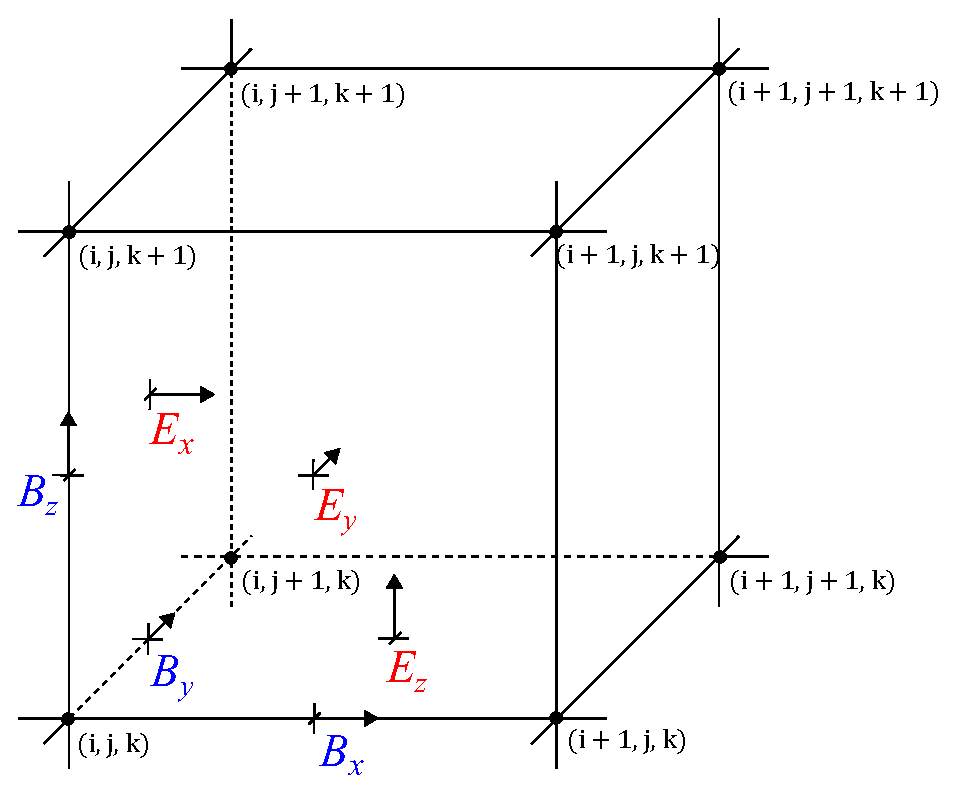
\includegraphics[width=0.355\paperwidth]{./img/YEE/yee.eps}
	\caption{Standard Cartesian Yee cell used for FDTD method}
	\label{3.1.1.14}
\end{figure}
\begin{equation}
\label{3.1.1.7}
\frac{\vec{B}_{ijk}^{\,n + 1/2} - \vec{B}_{ijk}^{\,n - 1/2}}{\Delta t} = -\nabla^{-} \times \vec{E}_{ijk}^{\,n}.
\end{equation}
Notice that this scheme achieves second-order accuracy in both, space and time. Discrete operators $ \left(\nabla^{+}\right) $ and $ \left(\nabla^{-}\right) $ used in \ref{3.1.1.6} - \ref{3.1.1.7} act on a scalar field $ f_{i j k} $ as follows,
\begin{equation}
\label{3.1.1.8}
\nabla^{+} f_{i j k} = \left(\frac{f_{i + 1,\: j,\: k} - f_{i,\: j,\: k}}{\Delta x}, \frac{f_{i,\: j + 1,\: k} - f_{i,\: j,\: k}}{\Delta y}, \frac{f_{i,\: j,\: k + 1} - f_{i,\: j,\: k}}{\Delta z} \right), 
\end{equation}
\begin{equation}
\label{3.1.1.9}
\nabla^{-} f_{i j k} = \left(\frac{f_{i,\: j,\: k} - f_{i - 1,\: j,\: k}}{\Delta x}, \frac{f_{i,\: j,\: k} - f_{i,\: j - 1,\: k}}{\Delta y}, \frac{f_{i,\: j,\: k} - f_{i,\: j,\: k - 1}}{\Delta z} \right).
\end{equation}
These operators have the following properties,
\begin{equation}
\label{3.1.1.10}
\nabla^{-} \cdot \nabla^{-} \times = \nabla^{+} \cdot \nabla^{+} \times = 0, \qquad \nabla^{-} \cdot \nabla^{+} = \nabla^{+} \cdot \nabla^{-} = \Delta^{\pm}.
\end{equation}
Symbol $ \Delta^{\pm} $ stands for the discrete Laplace operator in central differences,
\begin{equation}
\label{3.1.1.11}
\Delta^{\pm} f_{i, j, k} = \frac{f_{i - 1, j, k} + 2 f_{i, j, k} + f_{i + 1, j, k}}{\Delta x^{2}} + \frac{f_{i, j - 1, k} + 2 f_{i, j, k} + f_{i, j + 1, k}}{\Delta y^{2}} + \frac{f_{i, j, k - 1} + 2 f_{i, j, k} + f_{i, j, k + 1}}{\Delta z^{2}}.
\end{equation}

Before trying to find the solution of discretized Maxwell equations \ref{3.1.1.6} - \ref{3.1.1.7}, one must realize that this system of equations is not independent. In the three-dimensional case, there are eight first-order differential equations, but only six unknown vector components. Acting on the equations \ref{3.1.1.16} and \ref{3.1.1.7} by operators $ \left(\nabla^{-}\cdot\right) $ and $ \left(\nabla^{+}\cdot\right) $, respectively, one obtains
\begin{equation}
\label{3.1.1.12}
\frac{\nabla^{-} \cdot \vec{B}_{ijk}^{\,n + 1/2} - \nabla^{-} \cdot \vec{B}_{ijk}^{\,n - 1/2}}{\Delta t} = 0,
\end{equation}
\begin{equation}
\label{3.1.1.13}
\frac{\rho_{ijk}^{\,n + 1} - \rho_{ijk}^{\,n}}{\Delta t} + \nabla^{+} \cdot \vec{J}_{ijk}^{\,n + 1/2} = 0.
\end{equation}
It means that it is possible to solve only the equations \ref{3.1.1.16} and \ref{3.1.1.7}, while the divergence equations \ref{3.1.1.6}, \ref{3.1.1.15} can be considered as the initial conditions. Note that in this case, the continuity equation in the finite differences (\ref{3.1.1.13}) has to be fulfilled.

\section{Particle and field weighting}
In order to solve the Maxwell's equations, as shown in the previous section of this chapter, one has to know the source terms produced by the motion of the charged particles. In other words, it is necessary to assign charge and current densities from the continuous macro-particle positions to the discrete grid points. This simulation step is usually referred to as particle weighting and it involves some form of interpolation.
 
According to the kinetic theory, charge density $ \rho\left(\vec{x}, t \right) $ and current density $ \vec{J}\left(\vec{x}, t \right) $ are given by the following integrals over the velocity space,
\begin{equation}
\label{3.1.2.1}
\rho\left(\vec{x}, t \right) = \sum_s q_s \int f_s \left(\vec{x}, \vec{v}, t \right) \mathrm{d} \vec{v}, \qquad \vec{J}\left(\vec{x}, t \right) = \sum_s q_s \int f_s \left(\vec{x}, \vec{v}, t \right) \vec{v} \, \mathrm{d} \vec{v}.
\end{equation}
After discretization of \ref{3.1.2.1} using macro-particles and exploiting the properties of the shape functions, one gets immediately
\begin{equation}
\label{3.1.2.2}
\rho_{ijk}^{\,n} = \sum_{p} q_p S_{r}\left(\vec{r}_{ijk} - \vec{r}_{p}^{\,n}\right), \qquad \vec{J}_{ijk}^{\,n} = \sum_{p} q_p \vec{v}_p^{\,n} S_{r}\left(\vec{r}_{ijk} - \vec{r}_{p}^{\,n}\right),
\end{equation}
where $ q_p = q_s w_p $. However, using the formulas \ref{3.1.2.2} for charge and current deposition in PIC codes may violate the discrete continuity equation (\ref{3.1.1.13}) and in turn cause errors in Gauss's law (\ref{3.1.1.6}). In this case, one would have to solve the Poisson's equation for the correction of the electric field at every simulation time step or use a numerical scheme that satisfies the continuity equation exactly. These schemes are referred to as a charge conservation methods (\cite{villasenor}, \cite{esirkepov}, [source]).

Similarly, to advance macro-particle positions, as shown in the second section of this chapter, one has to know the force acting on them. Hence, it is necessary to assign electric and magnetic fields that are calculated at the discrete grid points to the continuous macro-particle positions. This simulation step is usually referred to as field weighting.

By analogy to the particle weighting, one may exploit the shape functions to calculate the spatial averages of the electric and magnetic field components,
\begin{equation}
\vec{E}_{p}^{\,n} = \sum_{ijk} \vec{E}_{ijk}^{\,n} S_{r}\left(\vec{r}_{ijk} - \vec{r}_{p}^{\,n}\right), \qquad \vec{B}_{p}^{\,n} = \sum_{ijk} \vec{B}_{ijk}^{\,n} S_{r}\left(\vec{r}_{ijk} - \vec{r}_{p}^{\,n}\right).
\end{equation}
Note that it is recommended to use the same weighting for both, particles and fields, in order to eliminate a self-force and ensure the conservation of momentum \cite{fehske}.



\section{Stability and accuracy}
The stability and accuracy of the standard PIC method is directly dependent on the size of the spatial and temporal simulation steps. In order to find correct parameters, one has to know the absolute accuracy and corresponding stability conditions.

The effect of the spatial grid is to smooth the interaction forces and to couple plasma perturbations to perturbations at other wavelengths, called aliases. It may lead to non-physical instabilities and numerical heating. To avoid these effects, the spatial step needs to resolve the Debye length (see \ref{2.1.3}). Thus, it is desirable to fulfill the following condition,
\begin{equation}
\Delta x, \Delta y, \Delta z \leq \lambda_{D}.
\end{equation}
In the general electromagnetic case, the time step has to satisfy the Courant--Fridrichs--Levy (CFL) condition \cite{jaroszynsky},
\begin{equation}
\label{3.1.4.1}
C = c^{2} \Delta t^{2} \left(\frac{1}{\Delta x^{2}} + \frac{1}{\Delta y^{2}} + \frac{1}{\Delta z^{2}}\right),
\end{equation}
where the dimensionless number $ C \leq 1 $ is called the CFL number. This condition limits the range of motion of all objects in the simulation during one time step. It ensures, that these particles would not cross more than one cell in one simulation time step. When this condition is violated, the growth of non-physical effects can be very rapid. 

The leap-frog scheme, used to solve the field equations and equations of motion, is second-order accurate in both, time and space. In addition, this scheme is explicit and time-reversible. A thorough study of PIC method can be found in [source].

\section{Extendable PIC Open Collaboration (EPOCH)}
The abbreviation EPOCH refers to an Extendable PIC Open Collaboration project \cite{bennett}. EPOCH is a multi-dimensional, relativistic, electromagnetic code designed for plasma physics simulations based on the PIC method. The code, which has been developed at University of Warwick, is written in FORTRAN and parallelized using MPI library \cite{MPI1994}. EPOCH is able to cover physical processes that may take place at ultra-high laser intensities, such as barrier suppression ionization, quantum electrodynamics emission and pair production.

The main computational features include dynamic load balancing option for making optimal use of all processors when run in parallel, allowing restart on an arbitrary number of processors. The setup of EPOCH is controlled through a customizable input deck. An input deck is a text file which can be used to set simulation parameters for EPOCH without necessity to edit or recompile the source code. Most aspects of the simulation can be controlled, such as the number of grid points in the simulation domain, the initial distribution of particles and the initial electromagnetic field configuration. In addition, EPOCH has been written to add more modern features and to structure the code in such a way that the future expansion of the code may be made as easily as possible. The entire core of the code uses SI units.

By default, EPOCH uses triangular particle shape functions with the peak located at the position of computational particle and a width of two cells, which provides relatively clean and fast solution. However, user can select higher order particle shape functions based on a spline interpolation by enabling compile-time option in the makefile.

The electromagnetic field solver uses FDTD scheme with second order of accuracy. The field components are spatially staggered on a standard Cartesian Yee cell \cite{yee}. The solver is directly based on the scheme derived by Hartmut Ruhl \cite{ruhl}. The particle pusher is relativistic, Birdsall and Landon type \cite{birdsall} and uses Villasenor and Buneman current weighting \cite{villasenor}.

EPOCH offers several types of boundary conditions for fields and particles, such as periodic, transmissive, reflecting and also Convolutional Perfectly Matched Layer (CPML) \cite{Roden2000, Taflove2000} boundary conditions. Laser beams can be attached to an arbitrary boundary via special boundary condition as well.

As a side project within this work, the code EPOCH has been instrumented to enable in situ diagnostics and visualization of the electromagnetic fields using ParaView Catalyst \cite{Ayachit2015}. The increasing demands of the simulations need more data to be stored on a disk and analysed. However, the capabilities of computing environment which is responsible for transferring the data and communication have not grown up as rapid as the computational power. Dumping and processing of all the data calculated during the simulation would take too much time, so in practice this usually means that they are stored only at several time steps or at much coarser resolution than the original data. The rest is just discarded and the significant part of information may be potentially lost.

In situ visualization describes techniques where data can be visualized in real-time as it is generated during a simulation and without it being stored on a storage resource. By coupling the visualization and simulation, the data transfer bottleneck can be overcome \cite{Bethel2012}. Furthermore, this approach allows scientists to monitor and interact with a running simulation, allowing for its parameters to be modified and allowing to immediately view the effects of these changes.

While a simulation is running, a user can see the size of the datasets that the simulation produces. But none of this data is physically stored on a storage system. The computationally expensive operations are carried out using ParaView’s \cite{Ayachit2015} graphical interface. So, the user can select data structures and analyze them in the same way as in post-processing. But there is one difference, the simulation is in progress so a user can observe the data as it is being generated. With Catalyst \cite{Ayachit2015}, it is also possible to pause the simulation or specify a break-point at a selected time step. This can be helpful if a user expects some interesting behavior of investigated phenomena or for identifying regions where numerical instability arises. For the implementation details, see appendix B.

The main goal of this work has been to implement a solution that would enable to simulate tightly focused laser beams using simulation code EPOCH \cite{bennett}. This will be closer described in the following chapter.



%-------------------------------------------------------------------------------

\chapter{Tight-focusing of laser pulses}
In this chapter, the achieved results of this work are presented and discussed. The code EPOCH, mentioned before, has been used for all simulations within this work. First, the boundary conditions for efficient absorption of hot electrons have been implemented and thoroughly tested in several test simulations. Second, two large-scale 2D simulations of laser-plasma interaction have been performed. The results have been post-processed and analyzed in terms of energy absorption efficiency, scattered radiation and production of hot electrons in the context of contemporary inertial fusion research.

\section{Laser boundary conditions}
In this section, another mathematical description of a focused laser beam based on a rigorous solution of the wave equation \ref{1.34} is presented. All the following calculations are reproduced from the excellent work of Illia Thiele et al. [source]. 

Assume that the laser beam propagates in vacuum without external sources along the z-axis of the Cartesian coordinate system. The wave equation \ref{1.34} in temporal Fourier space has the following form,
\begin{equation}
\label{4.1}
\laplace{\hat{\vec{E}}} \left(\vec{r}, \omega \right) + \frac{\omega^2}{c^2} \hat{\vec{E}} \left(\vec{r}, \omega \right) = 0,
\end{equation}
where the hat symbol placed on the top of a variable denotes the Fourier transform with respect to time. Next, one shall perform a spatial Fourier transform of \ref{4.1} with respect to transverse coordinates $ \vec{r_\bot} $ only,
\begin{equation}
\label{4.2}
\left(- k^2_x - k^2_y + \diffp[2]{}{z} \right) \bar{\vec{E}} \left(k_x, k_y, z, \omega \right) + \frac{\omega^2}{c^2} \bar{\vec{E}} \left(k_x, k_y, z, \omega \right) = 0,
\end{equation}
where the bar symbol placed on the top of a variable denotes the Fourier transform with respect to time and spatial transverse coordinates. The equation \ref{4.2} can be simplified as follows,
\begin{equation}
\label{4.3}
k^2_z \left(\vec{k}_\bot, \omega \right) \bar{\vec{E}}(\vec{k}_\bot, z, \omega) + \diffp[2]{}{z} \bar{\vec{E}} \left(\vec{k}_\bot, z, \omega \right) = 0.
\end{equation}
where $ k_z \left(\vec{k}_\bot, \omega \right) = \sqrt{-\vec{k}_\bot^2 + \omega^2/c^2} $ and $ \vec{k}_\bot = (k_x, k_y)^{\mathrm{T}} $. The fundamental solution of the equation \ref{4.3} consists of the forward $ (+) $ and backward $ (-) $ propagating waves,
\begin{equation}
\label{4.4}
\bar{\vec{E}}^{\pm} \left(\vec{k}_\bot, z, \omega \right) = \bar{\vec{E}}_{0}^{\pm} \left(\vec{k}_\bot, \omega \right) \e^{\pm \i k_z \left(\vec{k}_\bot, \omega \right) \left(z - z_0 \right)}.
\end{equation}
Where $ \bar{\vec{E}}_{0}^{\pm}\left(\vec{k}_\bot, \omega \right) $ is the electric laser field at some plane $ z = z_0 $. It might be clearly seen, that only two out of six vector components of the electric and magnetic fields are independent, therefore one may prescribe for example the transverse components $ \bar{\vec{E}}_{0, \bot}^{\pm}\left(\vec{k}_\bot, \omega \right) $ at the plane $ z = z_0 $ and all other components can be derived from the Maxwell's equations \ref{1.1}, \ref{1.3},
\begin{equation}
\label{4.5}
\bar{\vec{E}}^{\pm}_{\bot} \left(\vec{k}_\bot, z, \omega \right) = \bar{\vec{E}}^{\pm}_{0, \bot} \left(\vec{k}_\bot, \omega \right) \e^{\pm \i k_z \left(\vec{k}_\bot, \omega \right) \left(z - z_0 \right)},
\end{equation}
\begin{equation}
\label{4.6}
\bar{E}^{\pm}_z \left(\vec{k}_\bot, z, \omega \right) = \mp \frac{\vec{k}_\bot \cdot \bar{\vec{E}}^{\pm}_{\bot}(\vec{k}_\bot, z, \omega)}{k_z \left(\vec{k}_\bot, \omega \right)},
\end{equation}
\begin{equation}
\label{4.7}
\bar{\vec{B}}^{\pm}_{\bot} \left(\vec{k}_\bot, z, \omega \right) = \frac{1}{\omega k_z \left(\vec{k}_\bot, \omega \right)} \mathbb{R}^{\pm} \left(\vec{k}_\bot, \omega \right) \bar{\vec{E}}^{\pm} \left(\vec{k}_\bot, z, \omega \right),
\end{equation}
where
\begingroup
\renewcommand*{\arraystretch}{1.7}
\begin{equation}
\label{4.8}
\mathbb{R}^{\pm} \left(\vec{k}_\bot, \omega \right) =  \begin{pmatrix}
\mp k_x k_y & \mp \left[ k_z^2 \left(\vec{k}_\bot, \omega \right) + k_y^2 \right] & 0 \\
\pm \left[ k_z^2 \left(\vec{k}_\bot, \omega \right) + k_x^2 \right] & \pm k_x k_y & 0 \\
- k_y k_z \left(\vec{k}_\bot, \omega \right) & - k_x k_z \left(\vec{k}_\bot, \omega \right) & 0
\end{pmatrix}.
\end{equation} 
\endgroup

Analogically, one could solve the wave equation for the magnetic field \ref{1.35}, prescribe two transverse components of $ \bar{\vec{B}}_{0, \bot}^{\pm}\left(\vec{k}_\bot, \omega \right) $ at the plane $ z = z_0 $ and afterwards calculate all other fields using Maxwell's equations \ref{1.2}, \ref{1.4}. The complete proof, that the fields \ref{4.5} - \ref{4.7} are consistent with the Maxwell's equations in vacuum \ref{1.1} - \ref{1.4} can be found in the original paper [source].

Note that for $ k_\bot^2 > \omega^2/c^2 $, $ k_z \left(\vec{k}_\bot, \omega \right) $ becomes imaginary and equation \ref{4.4} describes evanescent waves that are unphysical in free space. Thus the Fourier spectrum of laser waves has to be filtered in the transverse Fourier space. On the other hand, if the spatial Fourier spectrum contains only components with $ k_\bot^2 \ll \omega^2/c^2 $, then $ k_z \left(\vec{k}_\bot, \omega \right) $ can be approximated using the first few terms of a Taylor series,
\begin{equation}
\label{4.9}
k_z \left(\vec{k}_\bot, \omega \right) \approx \frac{\abs{\omega}}{c} - \frac{c}{2 \abs{\omega}} k_\bot^2.
\end{equation}
Note that by plugging \ref{4.9} into equations \ref{4.5} - \ref{4.7} one gets the paraxial approximation.

In the last part of this section, the practical algorithm for implementation of the boundary conditions based on the previously derived solution of Maxwell's equations is presented. Assume that the laser beam propagates in a forward direction along the z-axis. In the beginning, it is necessary to prescribe the electric laser field $ \vec{E}_{0, \bot} (\vec{r}_{\bot}, t) $ in the plane $ \mathcal{P} $ at $ z = z_0 $. Note, that it can be defined by arbitrary function of space and time. The goal is then to find the fields $ \vec{E}_{\mathrm{B}} (\vec{r}_{\bot}, t) $ and $ \vec{B}_{\mathrm{B}} (\vec{r}_{\bot}, t) $ at the corresponding boundary $ z = z_\mathrm{B} $.

Consider that the transverse part of simulation domain is made of equidistant rectangular grid described by $ x^{i} $, $ y^{j} $, where $ i, j \in \left\lbrace 1, \ldots, N_{x, y} \right\rbrace $, and the grid steps $ \delta x $, $\delta y $. The simulation time $ t^{n} $, where $ n \in \left\lbrace 1, \ldots, N_{t} \right\rbrace $, is also divided into equidistant time steps of size $ \delta t $.

The algorithm allows to calculate fields $ \vec{E}_{\mathrm{B}}^{ij} (t) $ and $ \vec{B}_{\mathrm{B}}^{ij} (t) $ for any given time $ t $ from the interval $ \left[ t^{1} - \frac{z_\mathrm{B} - z_0}{c}, t^{N_t} - \frac{z_\mathrm{B} - z_0}{c} \right] $. In order to preserve clarity, the algorithm below is given in the exact form as in the original paper [source].

\begin{enumerate}
	\item Calculate $ \hat{\vec{E}}_{0, \bot}^{ijn} $ via discrete Fourier transforms in time:
	\begin{equation}
	\omega^n = \frac{2 \pi}{N_t \delta t} \left( -\frac{N_t}{2} + n \right),
	\end{equation}
	\begin{equation}
	\hat{\vec{E}}_{0, \bot}^{ijn} = \frac{\delta t}{2 \pi} \sum_{l=1}^{N_t} \vec{E}_{0, \bot}^{ijl} \e^{\i \omega^n t^l}, \quad n \in \left\lbrace 1, \dots, N_t \right\rbrace.
	\end{equation}
	\item Calculate $ \bar{\vec{E}}_{0, \bot}^{ijn} $ via two-dimensional discrete Fourier transforms in transverse space:
	\begin{equation}
	k_x^i = \frac{2 \pi}{N_x \delta x} \left( - \frac{N_x}{2} + i\right), \quad k_y^j = \frac{2 \pi}{N_y \delta y} \left( - \frac{N_y}{2} + j\right),
	\end{equation}
	\begin{equation}
	\bar{\vec{E}}_{0, \bot}^{ijn} = \frac{\delta x \delta y}{(2 \pi)^2} \sum_{l, m = 1}^{N_x, N_y} \hat{\vec{E}}_{0, \bot}^{lmn} \e^{- \i \: \left(k_x^i x^l + k_y^j y^m \right)}, \quad i, j \in \left\lbrace 1, \dots, N_{x, y} \right\rbrace.
	\end{equation}
	\item Calculate transverse electric field components at the boundary $ z = z_\mathrm{B} $:
	\begin{equation}
	k_z^{ijn} = \Re \sqrt{\frac{(\omega^n)^2}{c^2} - (k_x^i)^2 - (k_y^j)^2},
	\end{equation}
	\begin{equation}
	\bar{\vec{E}}_{\mathrm{B}, \bot}^{ijn} =
	\begin{cases} \bar{\vec{E}}_{0, \bot}^{ijn} \e^{\i k_z^{ijn}(z_\mathrm{B} - z_0)} & \text{for} \ k_z^{ijn} > 0 \\ 0 & \text{for} \ k_z^{ijn} = 0 \end{cases}.
	\end{equation}
	\item Calculate longitudinal electric field components at the boundary $ z = z_\mathrm{B} $:
	\begin{equation}
	\bar{E}_{\mathrm{B}, z}^{ijn} = \begin{cases} -\frac{k_x^i \bar{E}_{\mathrm{B}, x}^{ijn} + k_y^j \bar{E}_{\mathrm{B}, y}^{ijn}}{k_z^{ijn}} & \text{for} \ k_z^{ijn} > 0 \\ 0 & \text{for} \ k_z^{ijn} = 0 \end{cases}.
	\end{equation}
	\item Calculate the magnetic field at the boundary $ z = z_\mathrm{B} $:
	\begingroup
	\renewcommand*{\arraystretch}{1.7}
	\begin{equation}
	\mathbb{R}^{ijn} =  \begin{pmatrix}
	-k_x^i k_y^j & (k_x^i)^2 - (\omega^n)^2/c^2 \\
	(\omega^n)^2/c^2 - (k_y^j)^2 & k_x^i k_y^j \\
	-k_y^j k_z^{ijn} & k_x^i k_z^{ijn} 
	\end{pmatrix},
	\end{equation} 
	\endgroup
	\begin{equation}
	\bar{\vec{B}}_{\mathrm{B}}^{ijn} = \begin{cases} (\omega^n k_z^{ijn})^{-1} \mathbb{R}^{ijn} \bar{\vec{E}}_{\mathrm{B}, \bot}^{ijn} & \text{for} \ k_z^{ijn} > 0 \\ 0 & \text{for} \ k_z^{ijn} = 0 \end{cases}.
	\end{equation}
	\item Calculate $ \hat{\vec{E}}_{\mathrm{B}}^{ijn} $, $ \hat{\vec{B}}_{\mathrm{B}}^{ijn} $ via two-dimensional inverse discrete Fourier transforms:
	\begin{equation}
	\hat{\vec{E}}_{\mathrm{B}}^{ijn} = \frac{(2 \pi)^2}{N_x N_y \delta x \delta y} \sum_{l, m = 1}^{Nx, Ny} \bar{\vec{E}}_{\mathrm{B}}^{lmn} \e^{\i(k_x^l x^i + k_y^m y^j)},
	\end{equation}
	\begin{equation}
	\hat{\vec{B}}_{\mathrm{B}}^{ijn} = \frac{(2 \pi)^2}{N_x N_y \delta x \delta y}  \sum_{l, m = 1}^{Nx, Ny} \bar{\vec{B}}_{\mathrm{B}}^{lmn} \e^{\i(k_x^l x^i + k_y^m y^j)}.
	\end{equation}
	\item Calculate $ \vec{E}_{\mathrm{B}}^{ij}(t) $, $ \vec{B}_{\mathrm{B}}^{ij}(t) $ for any given time $ t \in [t^{1} - \frac{z_{\mathrm{B}} - z_{0}}{c}, t^{N_{t}}  - \frac{z_{\mathrm{B}} - z_{0}}{c}] $.
	\begin{equation}
	\vec{E}_{\mathrm{B}}^{ij} (t) = \frac{2 \pi}{N_t \delta t} \sum_{n = 1}^{N_t} \hat{\vec{E}}_{\mathrm{B}}^{ijn} \e^{-\i \omega^n t},
	\end{equation}
	\begin{equation}
	\vec{B}_{\mathrm{B}}^{ij} (t) = \frac{2 \pi}{N_t \delta t} \sum_{n = 1}^{N_t} \hat{\vec{B}}_{\mathrm{B}}^{ijn} \e^{-\i \omega^n t}.
	\end{equation}
\end{enumerate}

\section{Implementation}
One of the main goals of this work has been to implement the algorithm mentioned in the previous section, to evaluate its correctness in several test simulations and finally, to exploit resulting implementation for simulations of tightly focused Gaussian beams in laser-matter interaction. The main requirement on implementation has been easy to use with 2D version of particle-in-cell simulation code EPOCH [source]. For this reason, several possible solutions has been taken into account.

The final decision has been to create a static library, which will be able to compute desired quantities and will provide functions for communication with the main simulation code. The essential advantage is that it could be basically linked with any laser-plasma simulation code. Also, since it is necessary to call only two additional functions, the instrumentation will be fast, easy and the main simulation code will not be excessively disturbed. Furthermore, the implementation itself come with the CMake [source] support, which simplify the compilation process using platform and compiler independent configuration files.

The library has been written in C++ language and is object oriented so the algorithm can be easily extended to three dimensional geometry. In order to speedup the whole underlying computation, the algorithm has been parallelized using hybrid techniques. The time domain has been decomposed into the stripes corresponding to individual computational processes, the communication between these processes is ensured by MPI library. Furthermore, the computationally most expensive cycles are parallelized using OpenMP implementation of multi-threading. Later on, the speedup and parallel scaling performance will be briefly discussed.

Fourier transforms form the core of the computational process and their performance is crucial for the overall performance of the code. For this reason, many currently available libraries have been considered. Eventually, the Fourier transforms in the algorithm can be computed using FFTW [source] library, Intel$ ^{\scriptsize \textregistered} $ MKL [source] library or it is also possible to directly evaluate the formulas without using any additional library. The user specifies his option before the compilation. Regarding both libraries, a threaded versions of 1D in-place complex fast Fourier transforms have been used throughout the code. According to several measures, there is no significant difference between the speed of both implementations.

One potential bottleneck could happen during the computation of spatial Fourier transforms since the arrays with spatial data are decomposed into different processes. The cluster versions of functions performing the Fourier transforms have been tested, however they did not bring any significant speedup. The reason is as follows. They require to have the global array in memory and use its own distribution which involves overlapping. Since the size of global arrays is usually not so large and since it is necessary to perform a lot of different Fourier transforms, the majority of computational time is spent rather for communication, mainly if many of computational cores are used.

This issue has been solved by gathering the data on master process, performing the Fourier transforms in space by only one processor and scattering the data back to corresponding processes. This is the reason why the code does not scale well, however, the time to compute all desired quantities is in most cases negligible in comparison with the time required by main simulation cycle. Nevertheless, this issue could be improved in future.

Since it is necessary to compute the whole time evolution of the laser field at boundary for each grid point before the simulation starts, the resulting amount of data can be significantly large and does not have to fit in a computer memory. Thus, it is inevitable to dump the data into a file, which will be then accessed by the main simulation code. Due to the performance purposes, each computational process stores its data into a shared file with corresponding offset and in binary coding. Therefore, the output operations are as fast as possible and save the storage resources. Library then provide a function which allows to seek an arbitrary position in a file. This function is then called each time step of the main simulation loop to fill the laser source arrays with all the relevant data. This way of accessing data does not cause any significant slowdown or memory overhead.

The EPOCH [source] code require only transverse components of laser electric field, all other quantities are computed by the FDTD solver. The implementation of the library allows fully connection with EPOCH [source]. In practice, if the user wants to simulate tight-focusing, is is necessary to enable the corresponding flag as a compile-time option and then to specify all required parameters in the input file. The code then automatically computes all necessary data. It works generally regardless the number of lasers in the simulation or boundaries that they are attached to.

The current version of library does not work for obliquely incident laser pulses, because in this case one cannot exploit the advantage of an efficient computation with fast Fourier transforms. However, the code allows to compute the laser fields at boundary by evaluating Fourier integrals directly, so it could be easily extended. Second, it is at the moment possible to simulate only Gaussian laser pulses. However, the user can easily prescribe its own shape and position of the beam in focal plane by modifying corresponding part of the code.

Several most important data structures, functions and methods that form the core of the library for tight-focusing can be seen in appendix B.

\section{Evaluation}
\floatsetup[figure]{style=plain, subcapbesideposition=top}
\begin{figure}[h!]
	\centering
	\sidesubfloat[]{{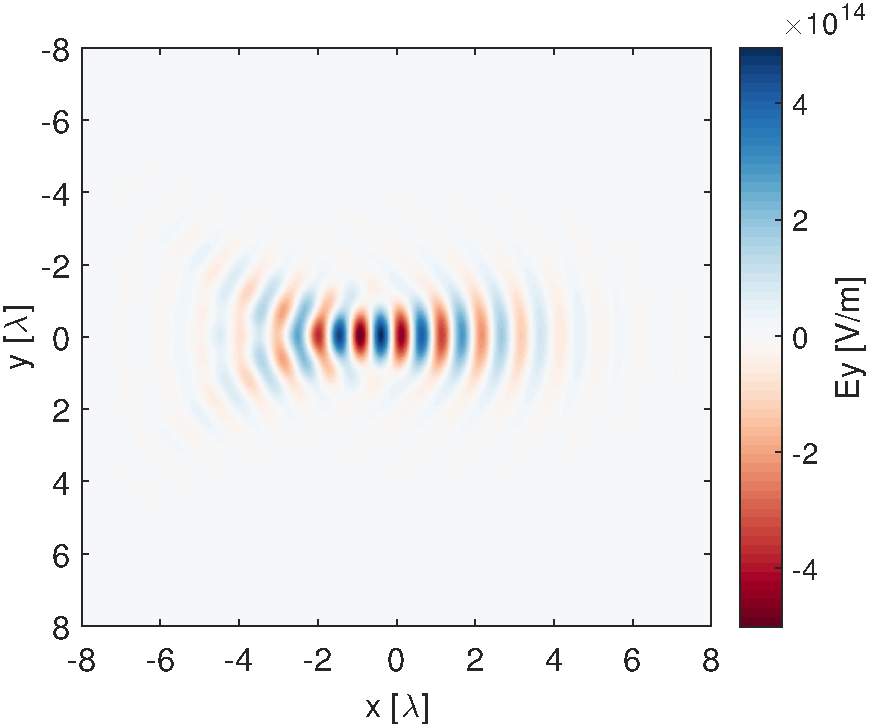
\includegraphics[width=0.44\linewidth]{./img/parax/Ey_focus.pdf}}}
	\hspace{2mm}
	\sidesubfloat[]{{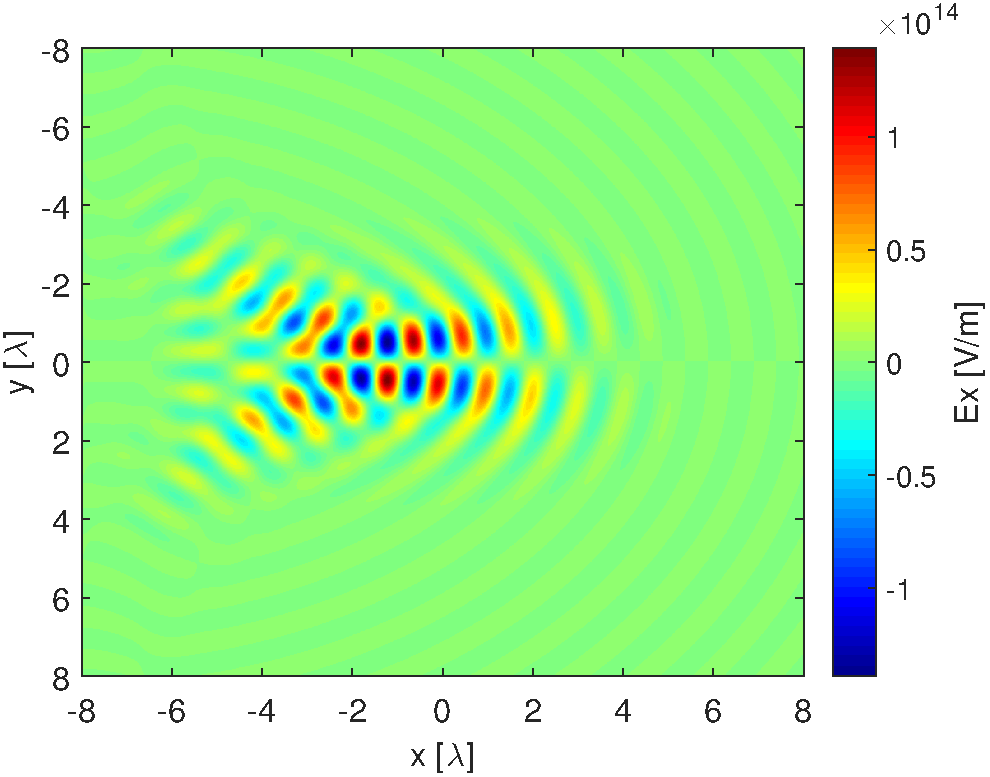
\includegraphics[width=0.44\linewidth]{./img/parax/Ex_focus.pdf}}}\\
	\sidesubfloat[]{{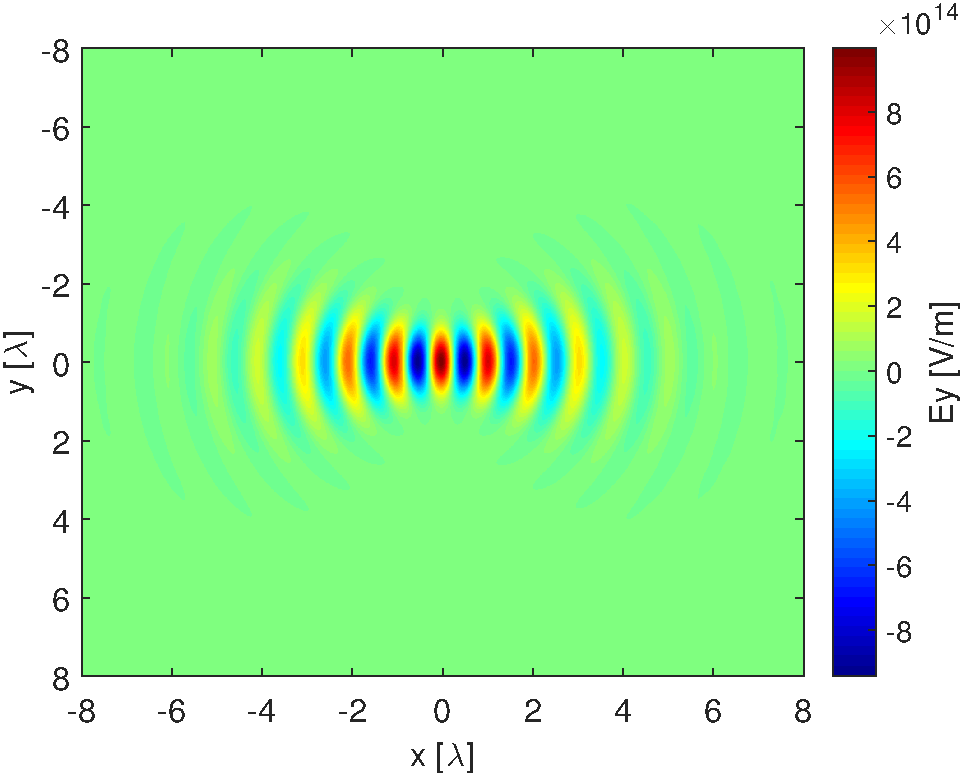
\includegraphics[width=0.44\linewidth]{./img/lbcs/Ey_focus.pdf}}}
	\hspace{2mm}
	\sidesubfloat[]{{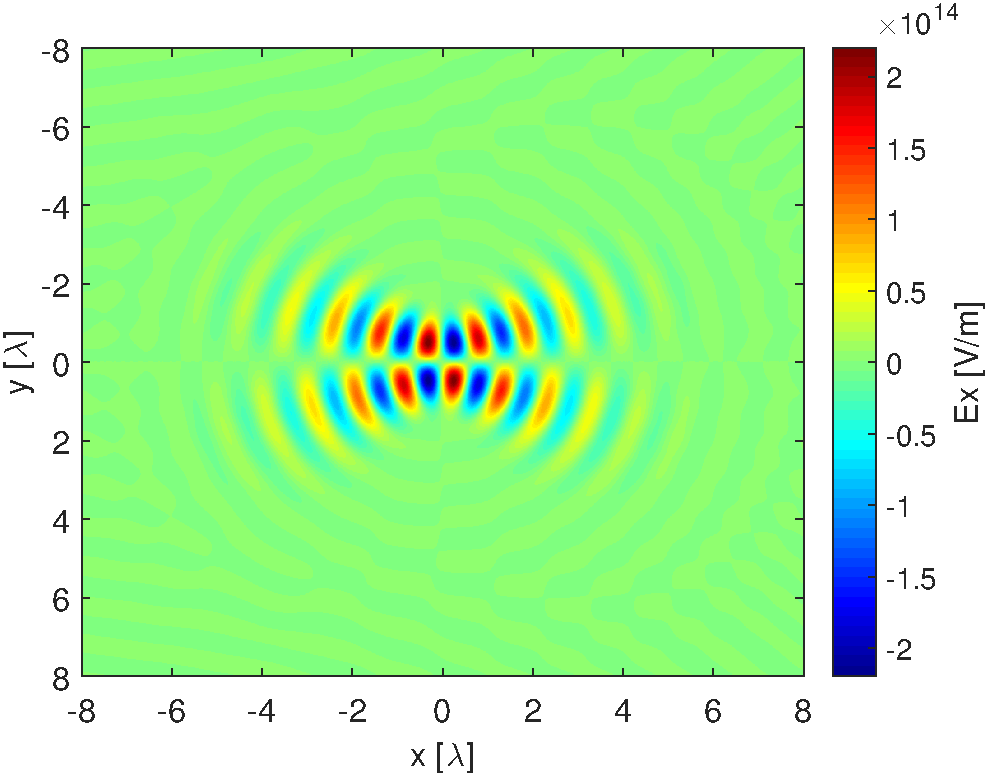
\includegraphics[width=0.44\linewidth]{./img/lbcs/Ex_focus.pdf}}}
	\caption{Transverse ($ E_{y} $) and longitudinal ($ E_{x} $) electric laser field components captured at the time step of their maximal intensity at the focal spot. The cases \textbf{(a)}, \textbf{(b)} correspond to the laser pulse propagating under the paraxial approximation, whilst \textbf{(c)}, \textbf{(d)} come from the simulation where the beam propagation has been resolved within the Maxwell consistent approach. In the case of paraxial approximation, both components reveal strong distortions and asymmetry, their focal spot is located about $ \mathrm{1 \lambda} $ closer to the left boundary than specified and the corresponding amplitude is significantly lower. The laser has been attached to the left hand side boundary.}
	\label{fig:1}
\end{figure}

To evaluate the correctness of the algorithm presented in the previous section of this chapter as well as to demonstrate the drawbacks of the paraxial approximation, several test simulations in 2D geometry have been performed. In the following text, a two limit cases are presented. The first pair of simulations employs tightly focused Gaussian laser beam with the size at focus comparable with the center laser wavelength, whilst the second one shows the case of the Gaussian beam with the size at focus one order of magnitude larger than the center laser wavelength, where both approaches should return identical results. Note, that all the simulations have been computed using 2D version of PIC code EPOCH [source] instrumented with library for tight-focusing.

\floatsetup[figure]{style=plain, subcapbesideposition=top}
\begin{figure}[h!]
	\centering
	\sidesubfloat[]{{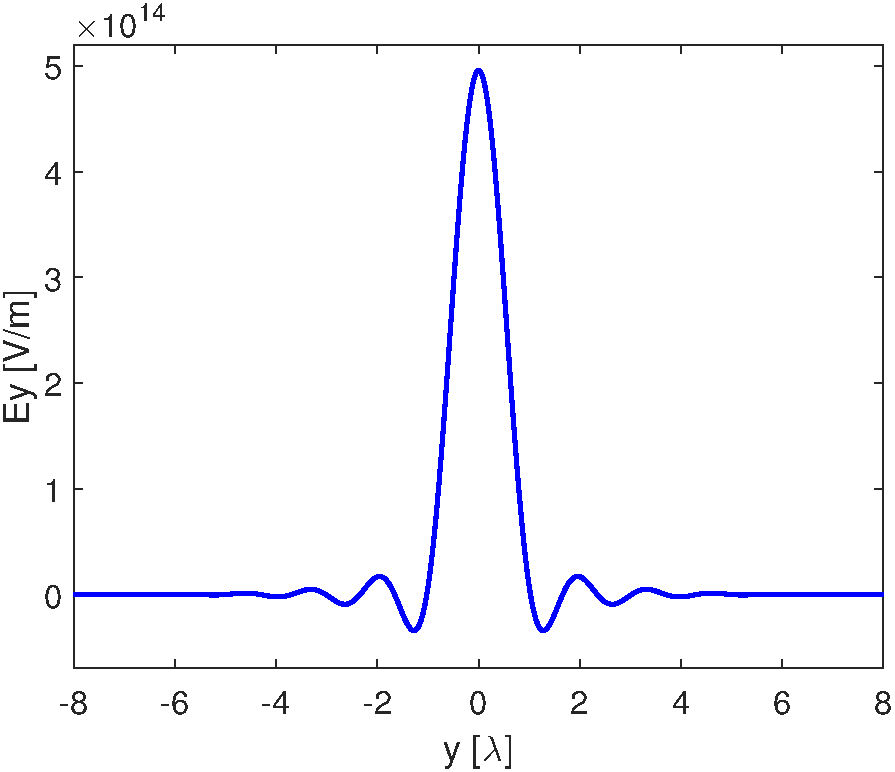
\includegraphics[width=0.4\linewidth]{./img/parax/Ey_focus_trans.pdf}}}
	\hspace{2mm}
	\sidesubfloat[]{{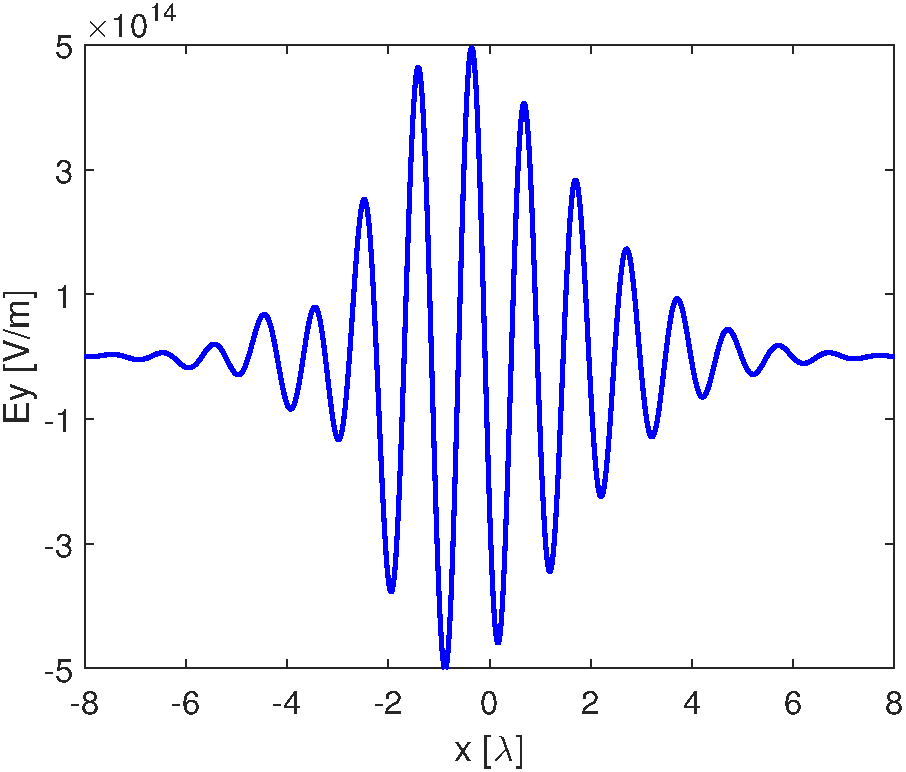
\includegraphics[width=0.4\linewidth]{./img/parax/Ey_focus_long.pdf}}}\\
	\sidesubfloat[]{{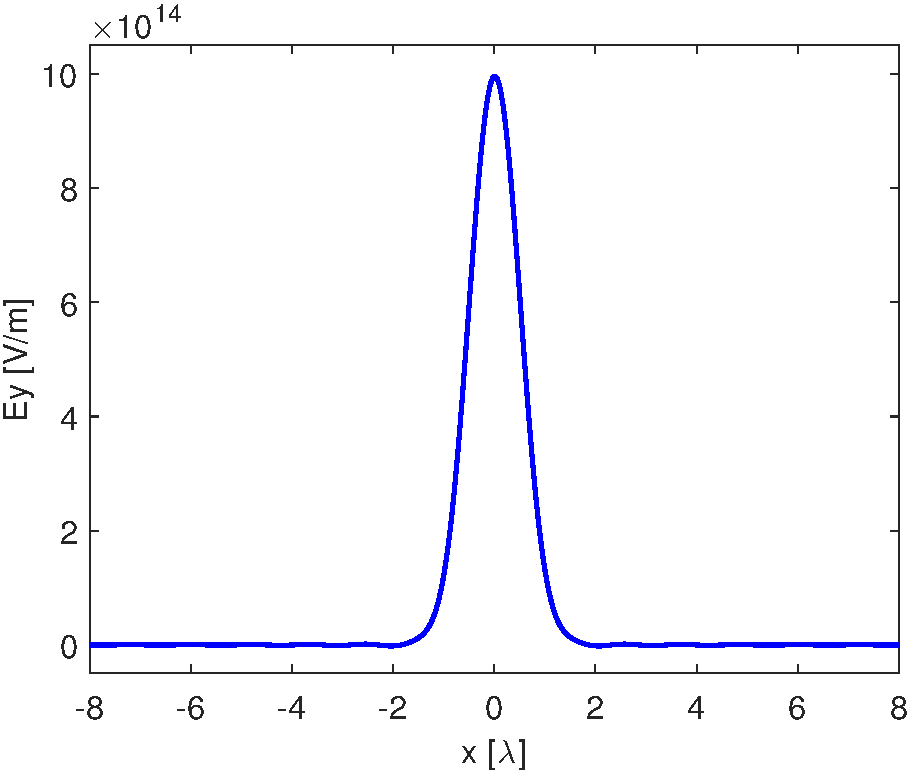
\includegraphics[width=0.4\linewidth]{./img/lbcs/Ey_focus_trans.pdf}}}
	\hspace{2mm}
	\sidesubfloat[]{{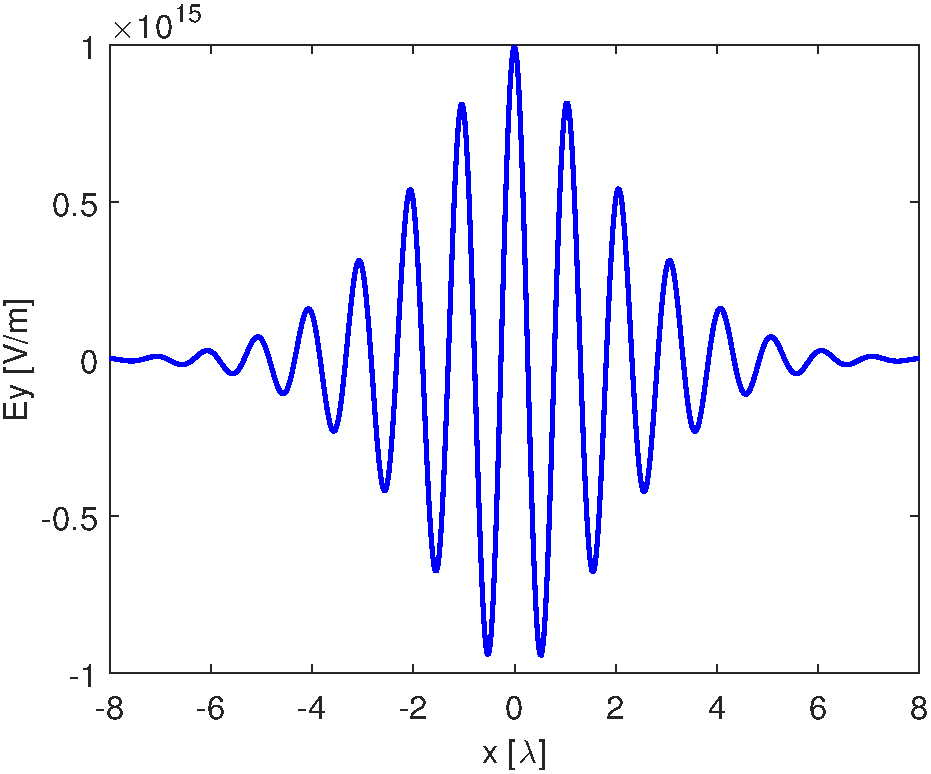
\includegraphics[width=0.4\linewidth]{./img/lbcs/Ey_focus_long.pdf}}}
	\caption{Transverse \textbf{(a)}, \textbf{(c)} and longitudinal \textbf{(b)}, \textbf{(d)} slices of the transverse electric laser field ($ E_{y} $) at the time step when it reaches maximal intensity at the focal spot. The cases \textbf{(a)}, \textbf{(b)} correspond to the laser pulse propagating under the paraxial approximation, whilst \textbf{(c)}, \textbf{(d)} come from the simulation where the beam propagation has been resolved within the Maxwell consistent approach. In the case of paraxial approximation, one can clearly see strong side-wings in the spatial beam profile \textbf{(a)} as well as the asymmetry of the field in the longitudinal line-out \textbf{(b)}.}
	\label{fig:2}
\end{figure}

First, have a look at the simulation of a tightly focused Gaussian beam. The p-polarized laser pulse with center wavelength $ \lambda = 1 \: \mathrm{\mu m} $ propagates from left hand side boundary to the right. Its duration has been chosen to $ \tau = 20 \: \mathrm{fs} $ in FWHM and amplitude $ E_0 = 1 \cdot 10^{15} \: \mathrm{V/m} $. The beam waist $ w_0 = 0.7 \: \mathrm{\mu m} $ is shorter than the laser wavelength, which implies that non-negligible parts of $ \bar{\vec{E}}_{0, \bot}(k_x, \omega) $ are evanescent. The focus is located at a distance $ x = 8 \: \mathrm{\mu m} $ from the boundary that the laser is attached to.

The size of the simulation domain is $ 16 \lambda \times 48 \lambda $, with 100 cells per laser wavelength in both directions, thus $ \Delta x = \Delta y = \lambda/100 = 10 \: \mathrm{nm} $. The one simulation time step is according to CFL condition $ \Delta t = 0.95 \sqrt{2} \lambda/ 100 c \approx 0.05 \: \mathrm{fs} $, the whole simulation time is then $ t = 150 \: \mathrm{fs} $. The pulse propagates in vacuum in order to get rid of all effects that could be potentially caused by plasma. All the simulation parameters can be found in the attached input files in the appendix A.

\floatsetup[figure]{style=plain, subcapbesideposition=top}
\begin{figure}[h!]
	\centering
	\sidesubfloat[]{{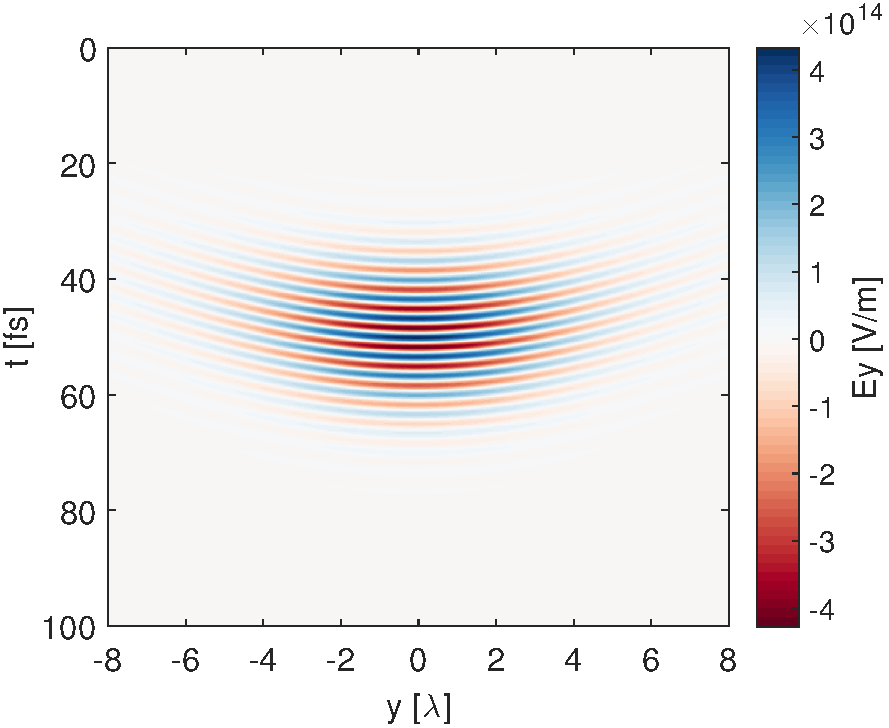
\includegraphics[width=0.44\linewidth]{./img/lbcs/Ey_boundary_time.pdf}}}
	\hspace{2mm}
	\sidesubfloat[]{{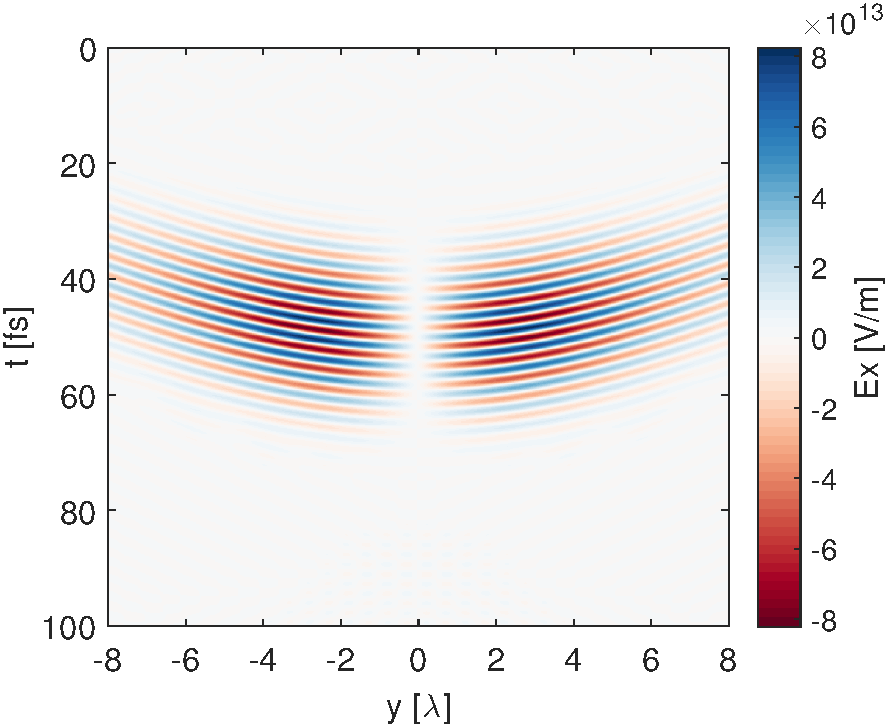
\includegraphics[width=0.44\linewidth]{./img/lbcs/Ex_boundary_time.pdf}}}
	\caption{The time evolution of transverse ($ E_{y} $) \textbf{(a)} and longitudinal ($ E_{x} $) \textbf{(b)} electric laser field components at the boundary that the laser is attached to. Both components has been calculated according to the Maxwell consistent approach.}
	\label{fig:3}
\end{figure}

\begin{figure}[h!]
	\centering
	\sidesubfloat[]{{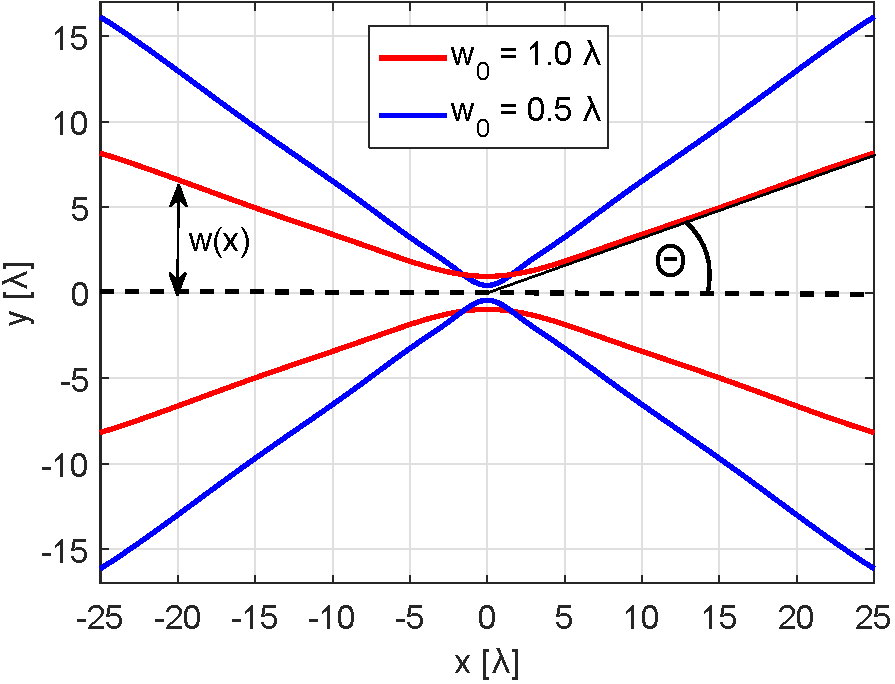
\includegraphics[width=0.435\linewidth]{./img/lbcs/divergence.pdf}}}
	\hspace{2mm}
	\sidesubfloat[]{{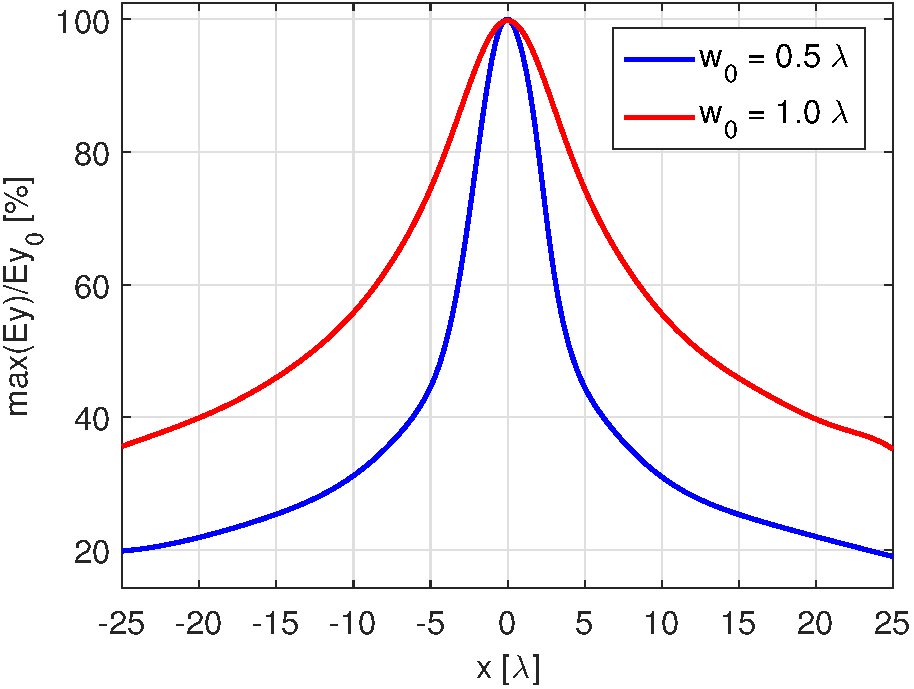
\includegraphics[width=0.445\linewidth]{./img/lbcs/amplitude.pdf}}}
	\caption{\textbf{(a)} Graph of the spot size parameter $ w(x) $ of the beams with $ w_0 = 1 \: \lambda $ and $ 0.5 \: \lambda $ calculated using Maxwell consistent approach. From the plotted lines, one can roughly estimate the beam divergence angle $ \Theta $. The divergence angles for both beams are surprisingly in a good accordance with the divergence angles of corresponding Gaussian beams. \textbf{(b)} Graph of the transverse ($ E_{y} $) electric laser field amplitude with respect to the distance from focal spot according to the Maxwell consistent approach. The values on vertical axis are given in a percentage of the amplitude at focus $ E_{0, y} $.}
	\label{fig:7}
\end{figure}

\floatsetup[figure]{style=plain, subcapbesideposition=top}
\begin{figure}[h!]
	\centering
	\sidesubfloat[]{{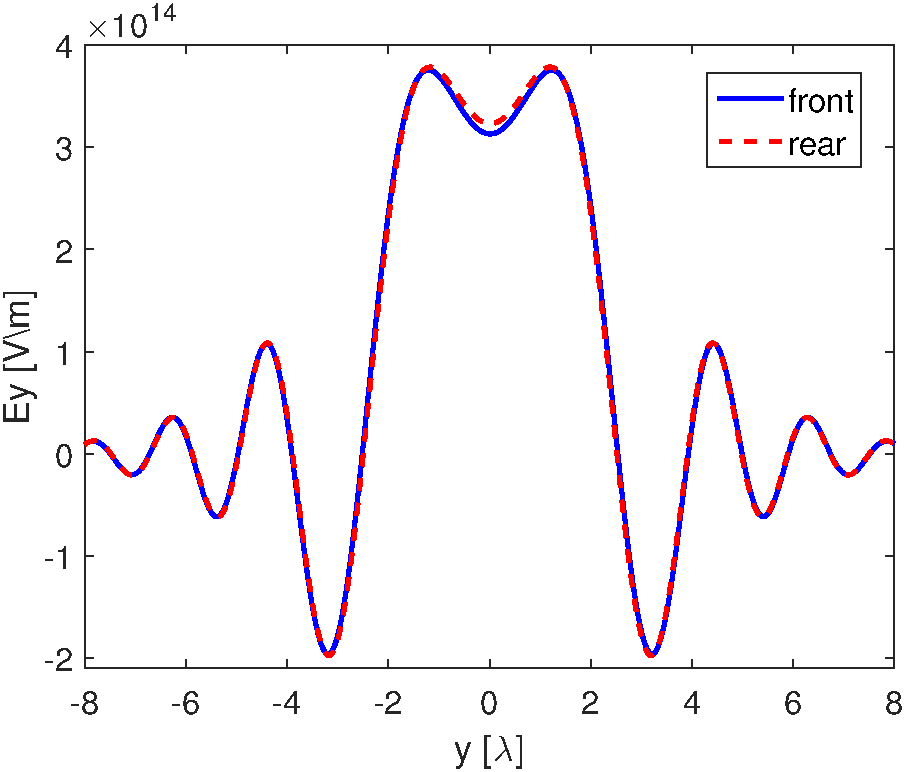
\includegraphics[width=0.44\linewidth]{./img/lbcs/Ey_boundary_trans.pdf}}}
	\hspace{1mm}
	\sidesubfloat[]{{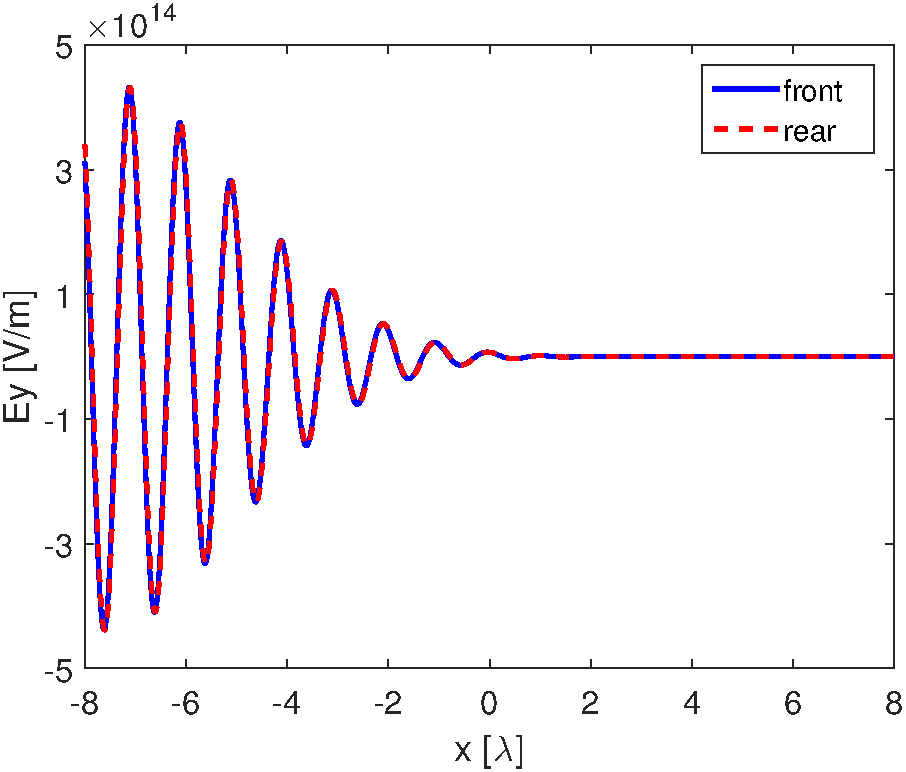
\includegraphics[width=0.44\linewidth]{./img/lbcs/Ey_boundary_long.pdf}}}
	\caption{Transverse \textbf{(a)} and longitudinal \textbf{(b)} slice of the transverse electric laser field ($ E_{y} $) when it reaches its maximal intensity at the front (blue) and rear (red) boundary. The results come from the simulation where the Maxwell consistent approach for laser propagation has been used. For better comparison, the field at the rear boundary in \textbf{(b)} has been horizontally flipped. The exact match between the field shapes at a different time steps of simulation proves the correctness of the laser beam propagation.}
	\label{fig:4}
\end{figure}

In the following paragraph, the results of the first simulation are discussed in a more detail. Fig. \ref{fig:1} shows transverse and longitudinal electric field components at their maximal intensity at focus for both cases, laser beam propagating under the paraxial approximation (Fig. \ref{fig:1} - a, b) and according to the approach consistent with Maxwell equations (Fig. \ref{fig:1} - c, d). In the case of paraxial approximation, one can clearly see strong distortions and asymmetry in the shape of both electric field components. In addition, the focus location is shifted about $ 1 \: \mathrm{\mu m} $ closer to the left boundary and the corresponding amplitude at focus is less than half the required value. In contrast, the fields produced by the simulation using Maxwell consistent calculation of laser fields at boundary are symmetric with respect to the focal spot and without any distortions. Furthermore, the focus location as well as the amplitude fulfills the initial requirements precisely.

Fig. \ref{fig:2} shows transverse and longitudinal slices of transverse electric field component at focus for the case of laser beam propagating under the paraxial approximation (Fig. \ref{fig:2} - a, b) as well as for the case where the beam propagation has been resolved within the Maxwell consistent approach (Fig. \ref{fig:2} - c, d). For the case of paraxial approximation, one can clearly see the asymmetry of the field shape in the longitudinal slice (Fig. \ref{fig:2} - b), which consequently leads to a decrease of the amplitude at focus and to the strong side-wings in the spatial beam profile, as might be better seen from the transverse slice (Fig. \ref{fig:2} - a). On the other hand, Maxwell consistent approach calculates fields of perfect symmetry with respect to the focal spot (Fig. \ref{fig:2} - c) and no side-wings or distortions are present (Fig. \ref{fig:2} - d).

\floatsetup[figure]{style=plain, subcapbesideposition=top}
\begin{figure}[h!]
	\centering
	\sidesubfloat[]{{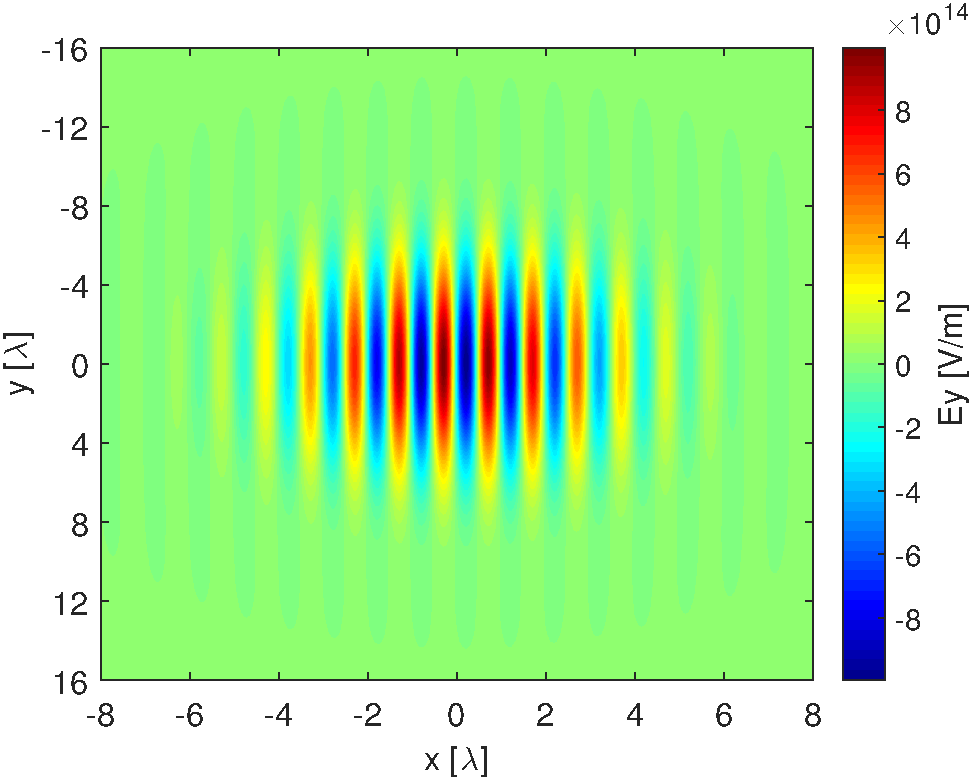
\includegraphics[width=0.45\linewidth]{./img/parax/Ey_focus_5mic.pdf}}}
	\hspace{2mm}
	\sidesubfloat[]{{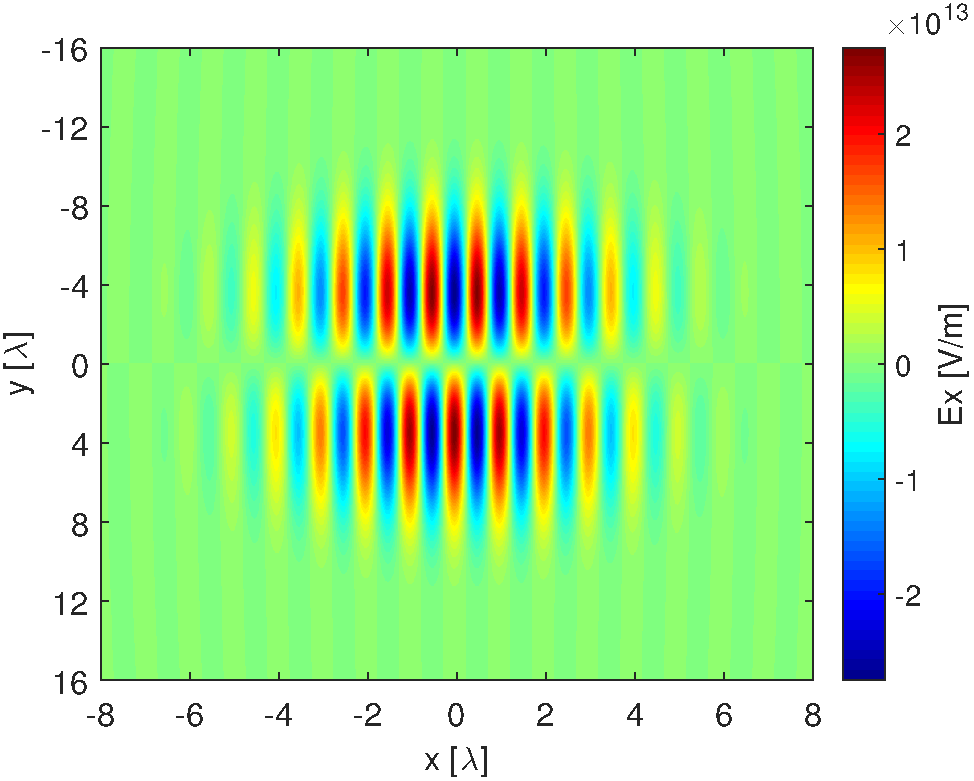
\includegraphics[width=0.44\linewidth]{./img/parax/Ex_focus_5mic.pdf}}}\\
	\sidesubfloat[]{{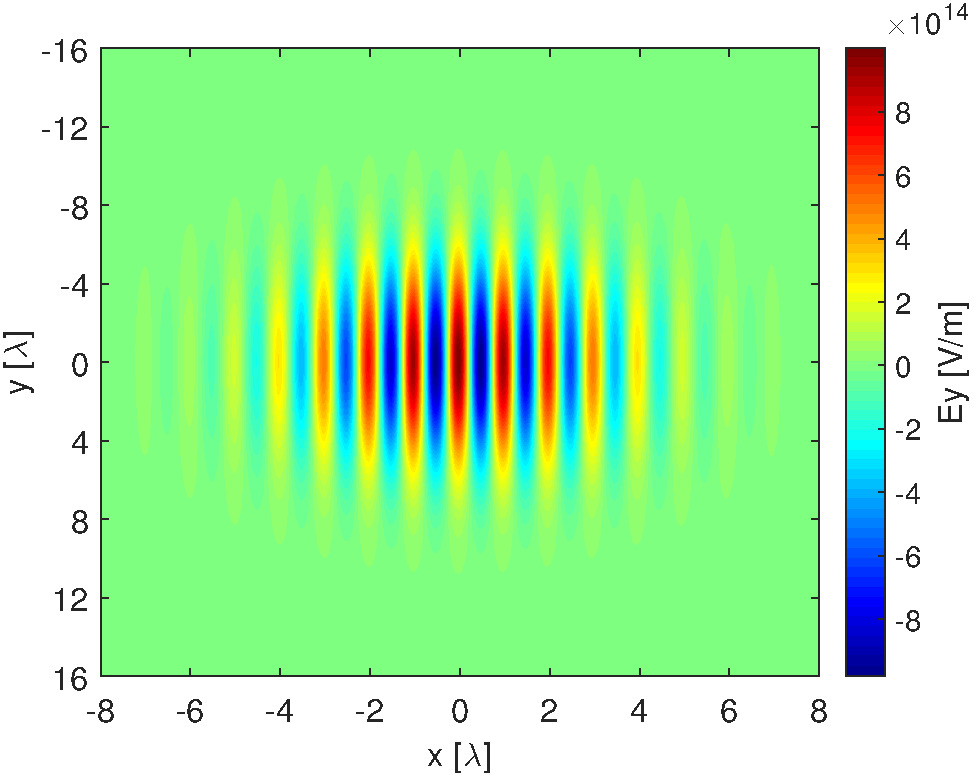
\includegraphics[width=0.44\linewidth]{./img/lbcs/Ey_focus_5mic.pdf}}}
	\hspace{2mm}
	\sidesubfloat[]{{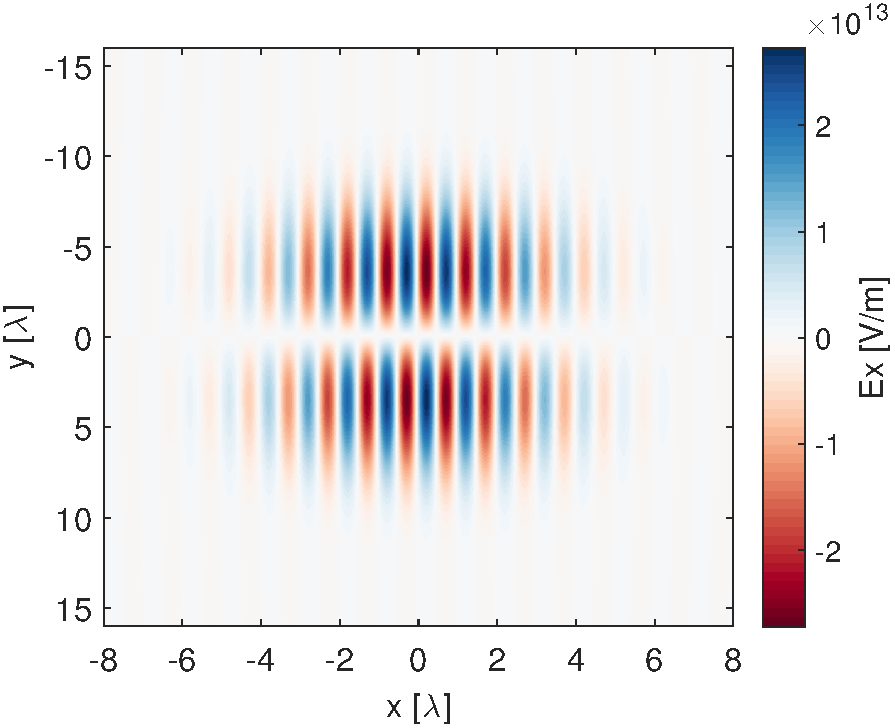
\includegraphics[width=0.43\linewidth]{./img/lbcs/Ex_focus_5mic.pdf}}}
	\caption{Transverse ($ E_{y} $) and longitudinal ($ E_{x} $) electric laser field components captured at the time step of their maximal intensity at the focal spot. The cases \textbf{(a)}, \textbf{(b)} correspond to the laser pulse propagating under the paraxial approximation, whilst \textbf{(c)}, \textbf{(d)} come from the simulation where the beam propagation has been resolved within the Maxwell consistent approach. The size of the focus has been chosen to be one order of the magnitude larger than the center laser wavelength. One can clearly see, that there is no significant difference between the shapes of the electric field components.}
	\label{fig:5}
\end{figure}

In Fig. \ref{fig:3} one can examine the time evolution of transverse (Fig. \ref{fig:3} - a) and longitudinal (Fig. \ref{fig:3} - b) electric field components at boundary as computed using Maxwell consistent approach. Note, that one have to chose carefully the transverse size of the domain, since the beam width at boundary may be much larger than at focus because of a diffraction. To estimate the beam width at boundary, one has to know the beam divergence angle $ \Theta $. In Fig. \ref{fig:7} - a, one can find a graph of the spot size parameter $ w $ as calculated using the Maxwell consistent approach for the beams focused to $ w_0 = 1 \: \lambda $ and $ 0.5 \: \lambda $. From the plotted lines, one can roughly estimate the beam divergence angle $ \Theta $. For the beam focused to $ w_0 = 1 \: \lambda $, the beam divergence angle has been around $ \Theta = 18.2 ^{\circ} $ which is almost identical value as for the Gaussian beam of the same parameters. For the beam with $ w_0 = 0.5 \: \lambda $ the divergence has been estimated to $ \Theta = 32.9 ^{\circ} $, while the Gaussian beam with the same size at focus has divergence $ \Theta = 36.5 ^{\circ} $. Consequently, in spite of the fact that the divergence of the tightly focused beams calculated using the Maxwell consistent approach is a little bit lower, both approaches are in quite a good accordance regarding this parameter.

In Fig. \ref{fig:7} - b, one can see the amplitude of the transverse electric laser field with respect to the distance from the focal spot calculated using Maxwell consistent approach. This could be particularly useful for experimenters since it is not always easy to focus the beam onto the target surface perfectly. 

\floatsetup[figure]{style=plain, subcapbesideposition=top}
\begin{figure}[h!]
	\centering
	\sidesubfloat[]{{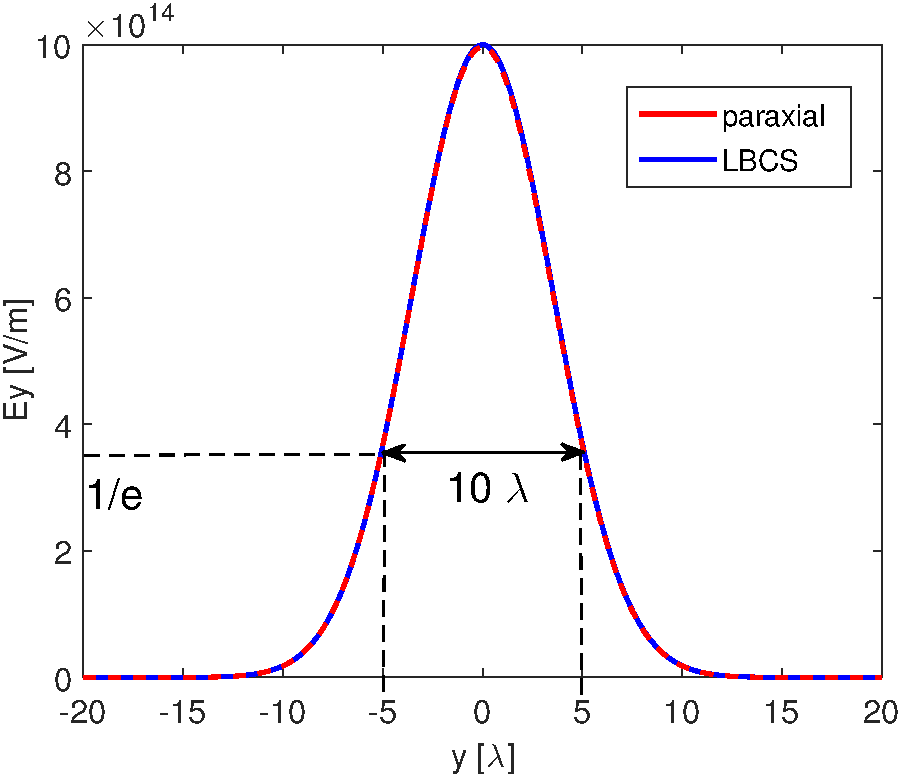
\includegraphics[width=0.44\linewidth]{./img/parax/Ey_focus_trans_comparison.pdf}}}
	\hspace{1mm}
	\sidesubfloat[]{{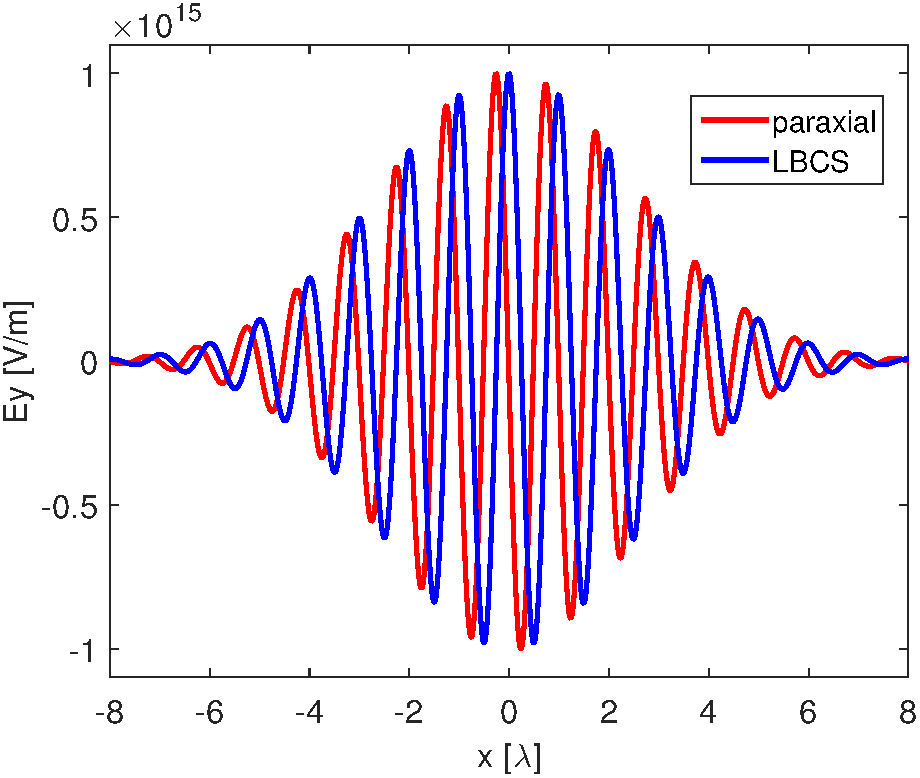
\includegraphics[width=0.45\linewidth]{./img/parax/Ey_focus_long_comparison.pdf}}}
	\caption{Transverse \textbf{(a)} and longitudinal \textbf{(b)} slices of the transverse electric laser field ($ E_{y} $) at the time step when it reaches maximal intensity at focus. Red lines correspond to the laser pulse propagating under the paraxial approximation, whilst blue lines come from the simulation where the beam propagation has been resolved within the Maxwell consistent approach. The size of the focus has been chosen to be one order of magnitude larger than the center laser wavelength. In the case of paraxial approximation, the focus is slightly shifted closer to the left boundary \textbf{(b)}, otherwise the size of the focus as well as the amplitude is correct for both cases \textbf{(a)}.}
	\label{fig:6}
\end{figure}

To evaluate a correctness of the beam propagation using Maxwell consistent approach, several criteria has been defined. The correctness of the amplitude and beam waist as well as the right focus location has already been verified. Additional criteria has been set on a beam symmetry. In Fig. \ref{fig:4}, one can find a comparison of the transverse electric laser field component when it achieves its maximal intensity at front and rear boundary. One can clearly see the exact match between the field shapes at different time steps of the simulation in transverse (Fig. \ref{fig:4} - a) and longitudinal (Fig. \ref{fig:4} - b) slices. Moreover, all the aforementioned criteria has been fulfilled also in other simulations with different input parameters that are not presented here. Consequently, these observations prove the correctness of the propagation at least for the tightly focused Gaussian laser beams.

For the second simulation, all the input parameters remained the same except the beam waist. Now, the parameter $ w_0 = 5 \: \mathrm{\mu m} $, which is about the limit case for the beam propagating under the paraxial approximation. Thus, one would expect that the simulation results will be almost identical.

Similarly as in Fig. \ref{fig:1}, Fig. \ref{fig:5} shows again transverse and longitudinal electric field components at their maximal intensity at focus for both cases, laser beam propagating under the paraxial approximation (Fig. \ref{fig:5} - a, b) and according to the approach consistent with Maxwell equations (Fig. \ref{fig:5} - c, d). Here, one cannot register any difference between the results corresponding to both approaches.

Also, the transverse slice of the transverse electric laser field component at focus (Fig. \ref{fig:6} - a) shows the correct shape and amplitude for both cases. The longitudinal slice (Fig. \ref{fig:6} - b), however, points out the fact that the location of the focal spot is still a little bit shifted closer to the left hand side boundary. Nevertheless, this difference could be in practice neglected. At the end of the day, for the Gaussian beams propagating under the paraxial approximation, the beam diameter at focus should be at least one order of magnitude larger than the center laser wavelength.

In conclusion, one should be aware that the propagation of tightly focused laser pulses cannot be described by paraxial approximation. Above, it has been shown that for the beams focused to a spot with the size comparable to a center laser wavelength, paraxial approximation leads to a shifted location of the focus, asymmetric laser field profiles with distortions and lower amplitude. These deviations are far from negligible and have without any doubt strong impact on the laser-matter or laser-plasma interaction results. On the other hand, the propagation of tightly focused Gaussian laser beams prescribed at boundaries according to the Maxwell consistent approach has been proven to be correct.

\section{Experimental approaches}
In experiments, several ways how to focus laser beams have been proposed. 

Any optical system can be described by several parameters.

numerical aperture, focal length, f-number

Aperture is the main lens or mirror that gathers the light to a
focus. Aperture diameter, D, is commonly measured in inches,
millimeters, centimeters or even meters. The larger the aperture, the
more light the system gathers and the finer details it can see. The top
figure shows various aperture diameters for telescopes that can be
bought. In optics, the numerical aperture (NA) of an optical system is a dimensionless number that characterizes the range of angles over which the system can accept or emit light. By incorporating index of refraction in its definition, NA has the property that it is constant for a beam as it goes from one material to another, provided there is no optical power at the interface.

Focal length is the distance between the center of the aperture
and the point in space where distant light rays come to a focus. In the
figure, both a lens and a properly-curved mirror can have focal points.
The symbol, f, represents the focal length.

F/ number is a measure of the speed and clarity of the optical
system. It is the ratio of the focal distance to the aperture size. Fast
systems have small F/numbers such as F/1, F/2 or F/3. Slow systems
have large F/ numbers such as F/8, F/15 or even F/20. In photography
these are also called F-stops. The f-number of an optical system such as a camera lens is the ratio of the system's focal length to the diameter of the entrance pupil.[1] It is a dimensionless number that is a quantitative measure of lens speed



\floatsetup[figure]{style=plain, subcapbesideposition=top}
\begin{figure}[h!]
	\centering
	\sidesubfloat[]{{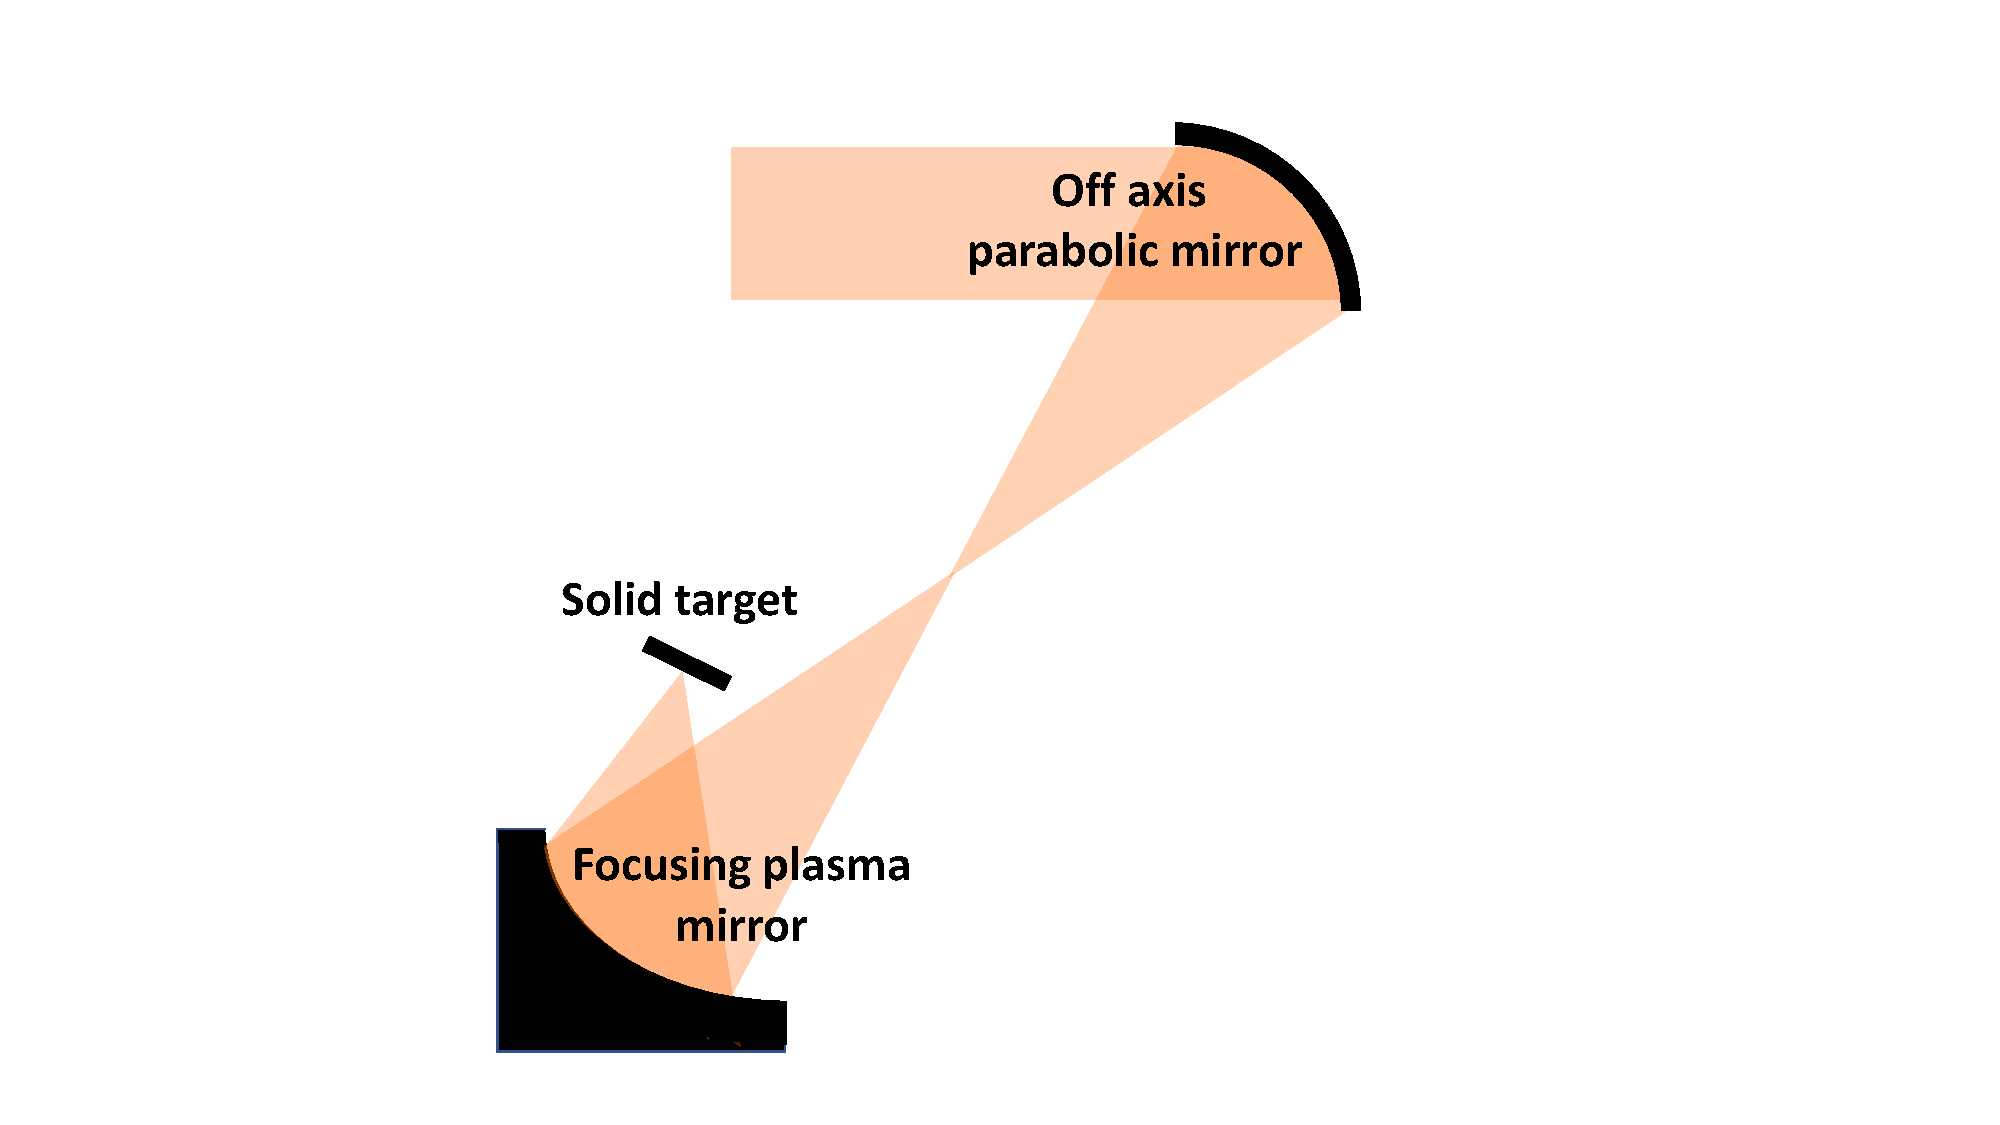
\includegraphics[width=0.35\linewidth]{./img/exp/diagram.pdf}}}
	\hspace{5mm}
	\sidesubfloat[]{{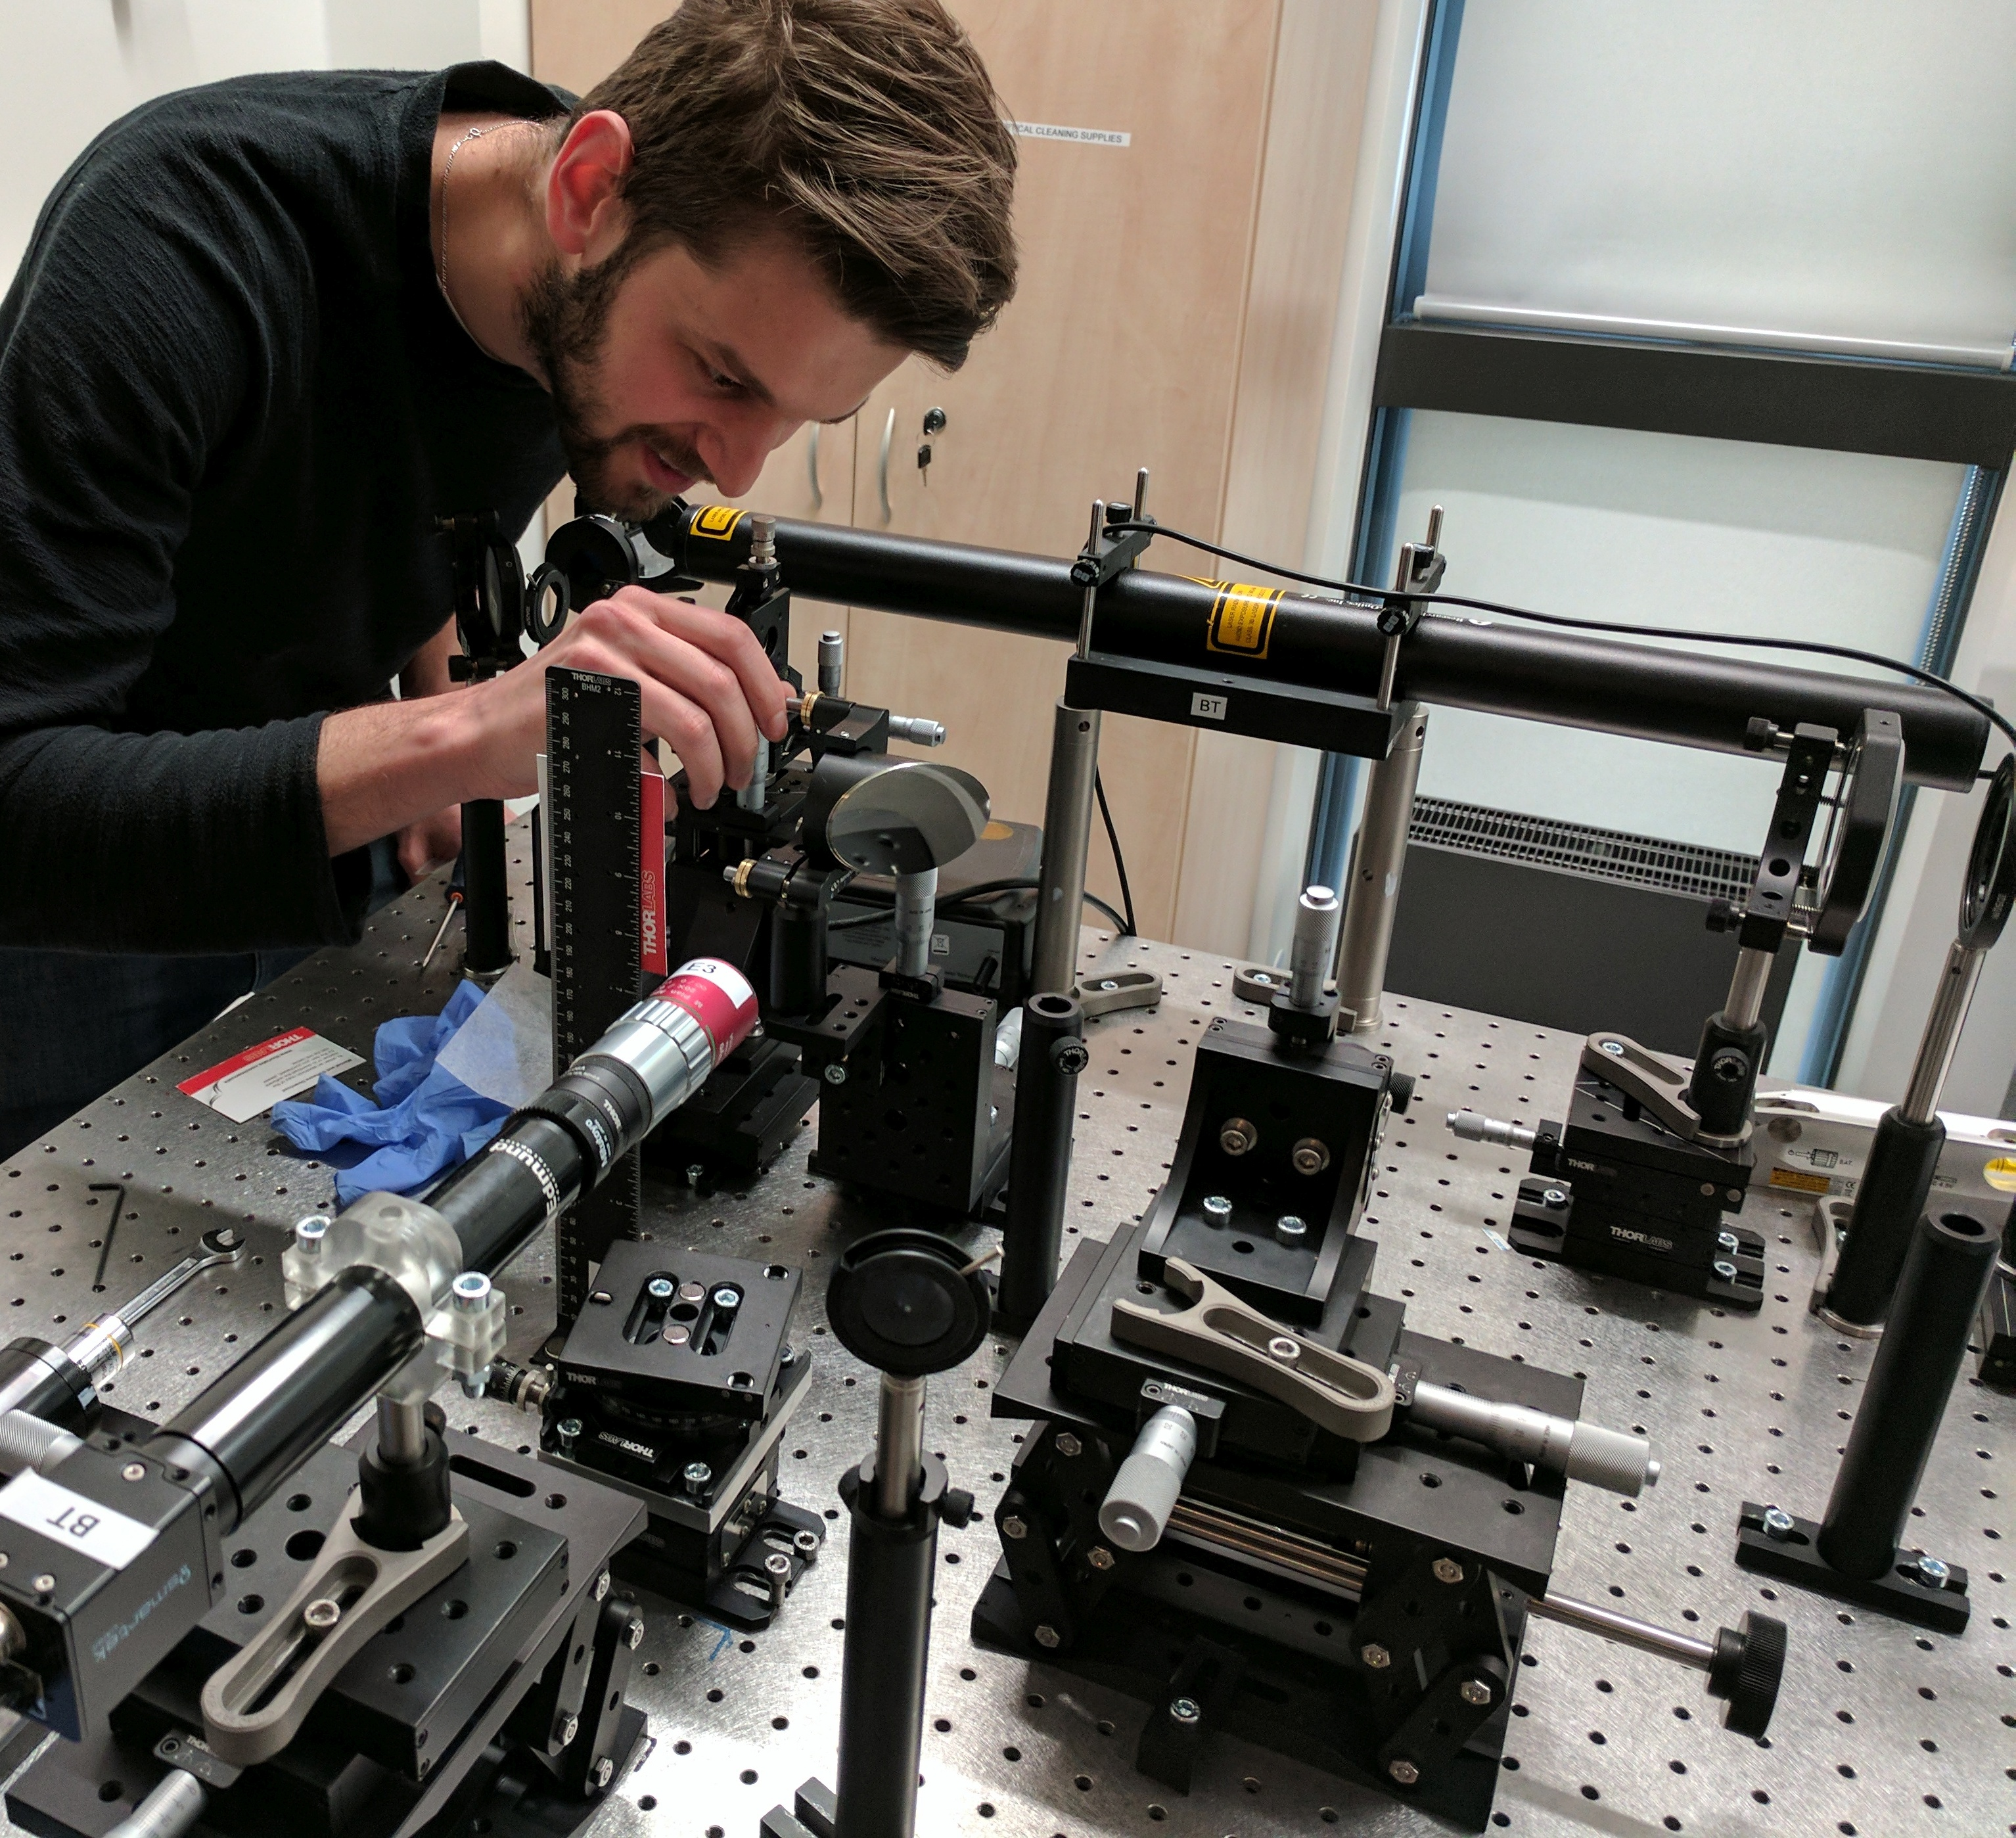
\includegraphics[width=0.4\linewidth]{./img/exp/photo2.jpg}}}
	\caption{}
	\label{}
\end{figure}

%-------------------------------------------------------------------------------

\chapter{Simulation results}
\noindent
First set (8 simulations const. int or const. e, traget 2 micron, 2000 ppc):
\noindent
Laser:
\begin{itemize}
	\item wavelength: $ \lambda $ = 0.8 $ \mu m $
	\item const intensity: I = 1e20 W/cm2 or const. energy: E = 2.8306e4 J (corresponds to I = 1e20 W/cm2 for $ w_0 $ = 1.0 $ \mu m $)
	\item duration: t = 30 fs (in FWHM)
	\item beam waist in focus: $ w_0 $ = 0.5, 1.0, 2.0, 4.0 $ \mu m $
	\item focus distance from boundary: $ x_\mathrm{B} - x_0 $ = 8 $ \mu m $
	\item polarization: P
	\item boundary: left 
\end{itemize}
Domain:
\begin{itemize}
	\item x min: 0 $ \mu m $
	\item x max: 15 $ \mu m $
	\item y min: -20 $ \mu m $
	\item y max: 20 $ \mu m $
	\item $ N_x $: 1875 cells ($ \delta x $ = $ \lambda/100 $ = 8 nm)
	\item $ N_y $: 5000 cells ($ \delta y $ = $ \lambda/100 $ = 8 nm)
	\item time step: $ \delta t $ = $ 1/(\sqrt{2} c) \lambda /100 \approx $ 0.05 fs 
	\item simulation time: $ \tau $ = 200 fs
\end{itemize}
Target:
\begin{itemize}
	\item x min: 8 $ \mu m $
	\item x max: 10 $ \mu m $
	\item y min: -15 $ \mu m $
	\item y max: 15 $ \mu m $
	\item electrons: 2000 ppc
	\item protons: 100 ppc
	\item density: 100 critical
	\item temperature: 100 eV
\end{itemize}

\noindent
Seconds set (2 simulations with higher intensity, 1000 ppc):
\noindent
Laser:
\begin{itemize}
	\item wavelength: $ \lambda $ = 0.8 $ \mu m $
	\item const intensity: I = 1e21 W/cm2
	\item duration: t = 30 fs (in FWHM)
	\item beam waist in focus: $ w_0 $ = 0.5, 2.0 $ \mu m $
	\item focus distance from boundary: $ x_\mathrm{B} - x_0 $ = 8 $ \mu m $
	\item polarization: P
	\item boundary: left 
\end{itemize}
Domain:
\begin{itemize}
	\item x min: 0 $ \mu m $
	\item x max: 15 $ \mu m $
	\item y min: -20 $ \mu m $
	\item y max: 20 $ \mu m $
	\item $ N_x $: 1875 cells ($ \delta x $ = $ \lambda/100 $ = 8 nm)
	\item $ N_y $: 5000 cells ($ \delta y $ = $ \lambda/100 $ = 8 nm)
	\item time step: $ \delta t $ = $ 1/(\sqrt{2} c) \lambda /100 \approx $ 0.05 fs 
	\item simulation time: $ \tau $ = 200 fs
\end{itemize}
Target:
\begin{itemize}
	\item x min: 8 $ \mu m $
	\item x max: 10 $ \mu m $
	\item y min: -15 $ \mu m $
	\item y max: 15 $ \mu m $
	\item electrons: 1000 ppc
	\item protons: 100 ppc
	\item density: 100 critical
	\item temperature: 100 eV
\end{itemize}

\noindent
Third set (2 simulations with higher intensity, thiner target (0.25 micron), 2000 ppc):
\noindent
Laser:
\begin{itemize}
	\item wavelength: $ \lambda $ = 0.8 $ \mu m $
	\item const intensity: I = 1e21 W/cm2
	\item duration: t = 30 fs (in FWHM)
	\item beam waist in focus: $ w_0 $ = 0.5, 2.0 $ \mu m $
	\item focus distance from boundary: $ x_\mathrm{B} - x_0 $ = 8 $ \mu m $
	\item polarization: P
	\item boundary: left 
\end{itemize}
Domain:
\begin{itemize}
	\item x min: 0 $ \mu m $
	\item x max: 15 $ \mu m $
	\item y min: -20 $ \mu m $
	\item y max: 20 $ \mu m $
	\item $ N_x $: 1875 cells ($ \delta x $ = $ \lambda/100 $ = 8 nm)
	\item $ N_y $: 5000 cells ($ \delta y $ = $ \lambda/100 $ = 8 nm)
	\item time step: $ \delta t $ = $ 1/(\sqrt{2} c) \lambda /100 \approx $ 0.05 fs 
	\item simulation time: $ \tau $ = 200 fs
\end{itemize}
Target:
\begin{itemize}
	\item x min: 8 $ \mu m $
	\item x max: 8.25 $ \mu m $
	\item y min: -15 $ \mu m $
	\item y max: 15 $ \mu m $
	\item electrons: 2000 ppc
	\item protons: 100 ppc
	\item density: 100 critical
	\item temperature: 100 eV
\end{itemize}

\floatsetup[figure]{style=plain, subcapbesideposition=top}
\begin{figure}[h!]
	\centering
	\sidesubfloat[]{{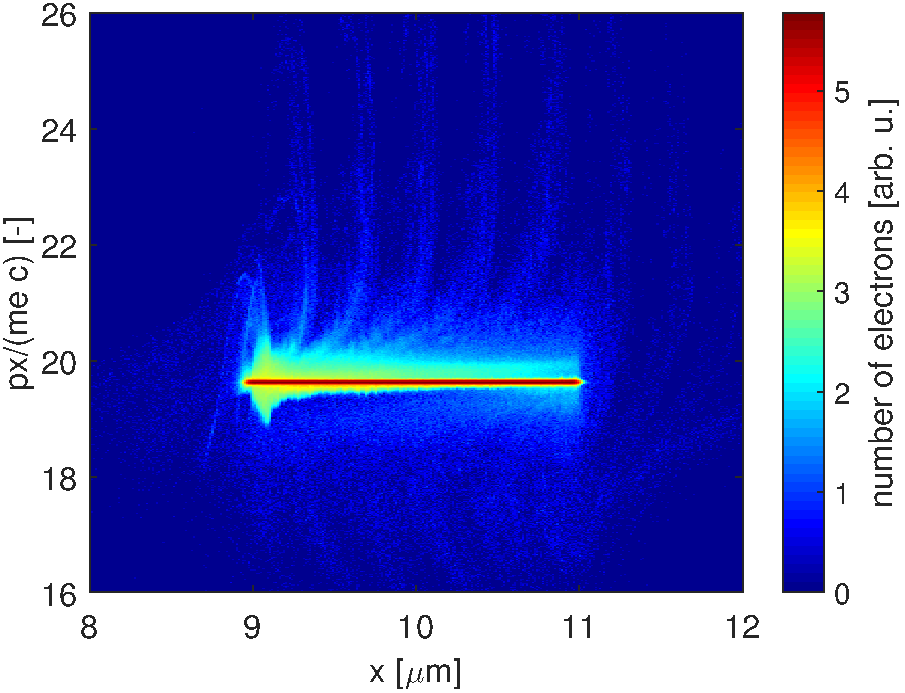
\includegraphics[width=0.45\linewidth]{./img/results/i1e20/05/x_px.pdf}}}
	\sidesubfloat[]{{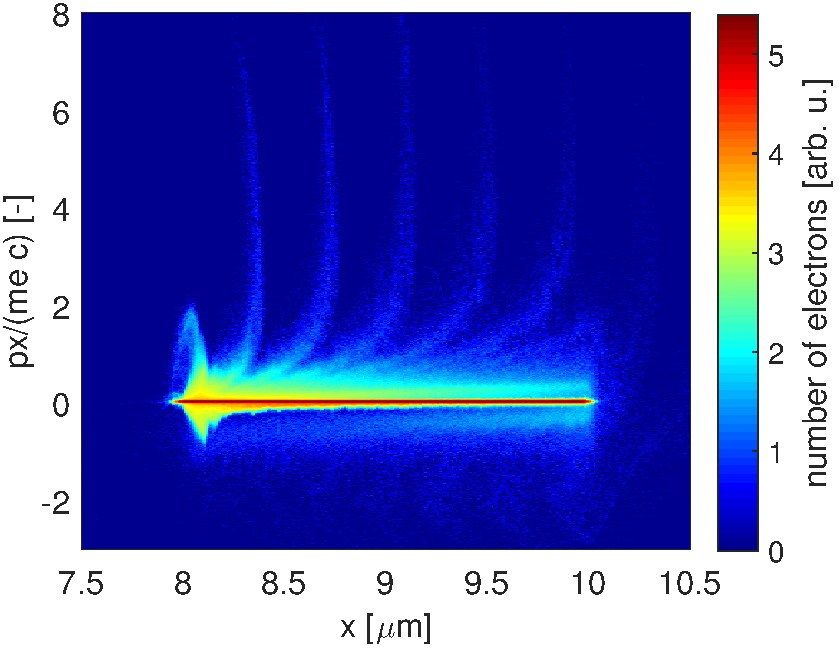
\includegraphics[width=0.45\linewidth]{./img/results/i1e20/2/x_px.pdf}}}\\
	\sidesubfloat[]{{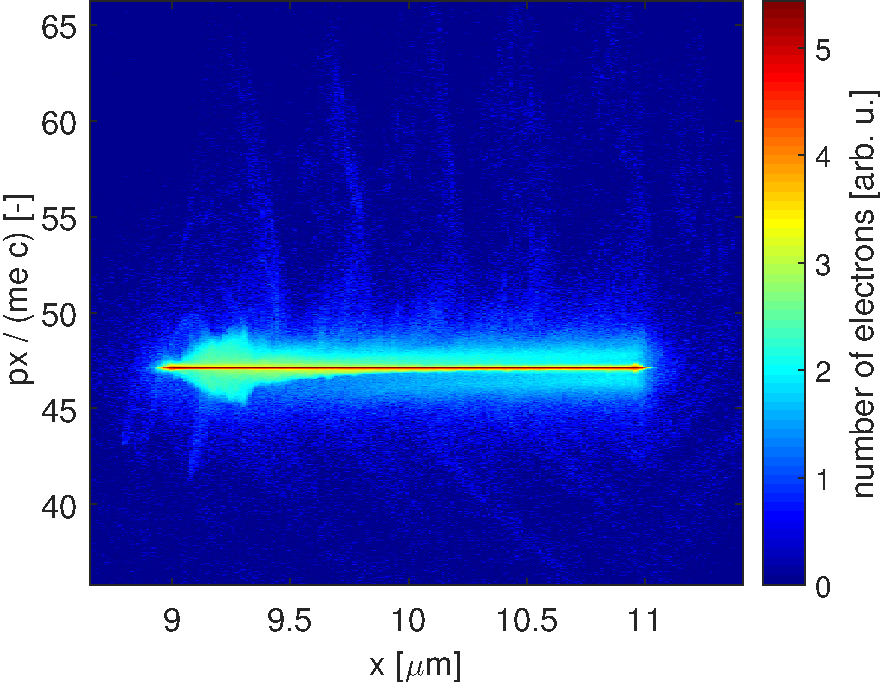
\includegraphics[width=0.45\linewidth]{./img/results/i1e21/05/x_px.pdf}}}
	\sidesubfloat[]{{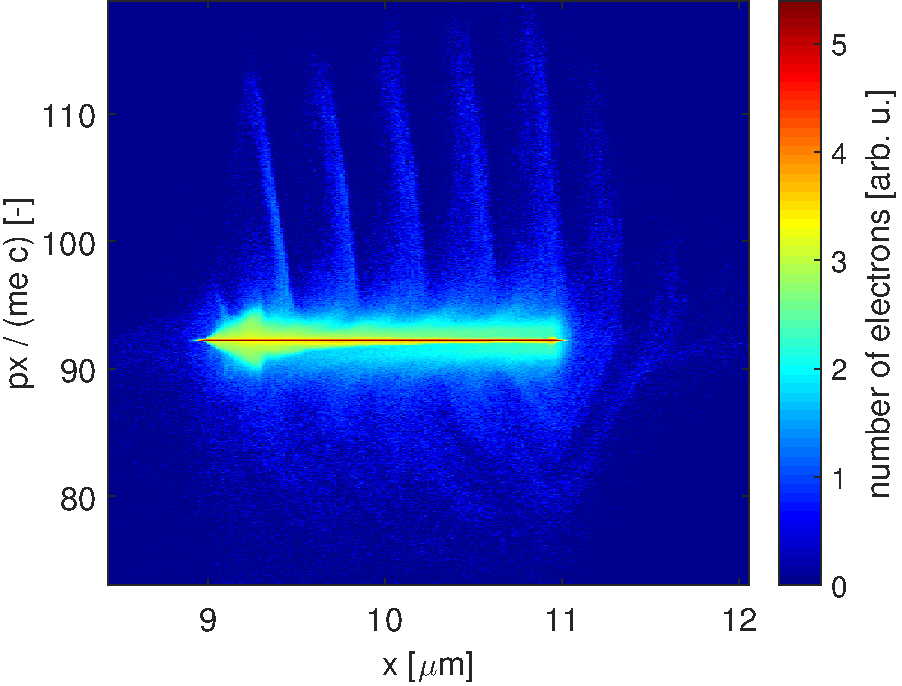
\includegraphics[width=0.45\linewidth]{./img/results/i1e21/2/x_px.pdf}}}
	\caption{\textbf{(a)} w0 = 05 micron, I = 1e20 W/cm2, t = 100 fs \textbf{(b)} w0 = 2 micron, I = 1e20 W/cm2, t = 100 fs \textbf{(c)} w0 = 05 micron, I = 1e21 W/cm2, t = 100 fs \textbf{(d)} w0 = 2 micron, I = 1e21 W/cm2, t = 100 fs}
	\label{}
\end{figure}

\floatsetup[figure]{style=plain, subcapbesideposition=top}
\begin{figure}[h!]
	\centering
	\sidesubfloat[]{{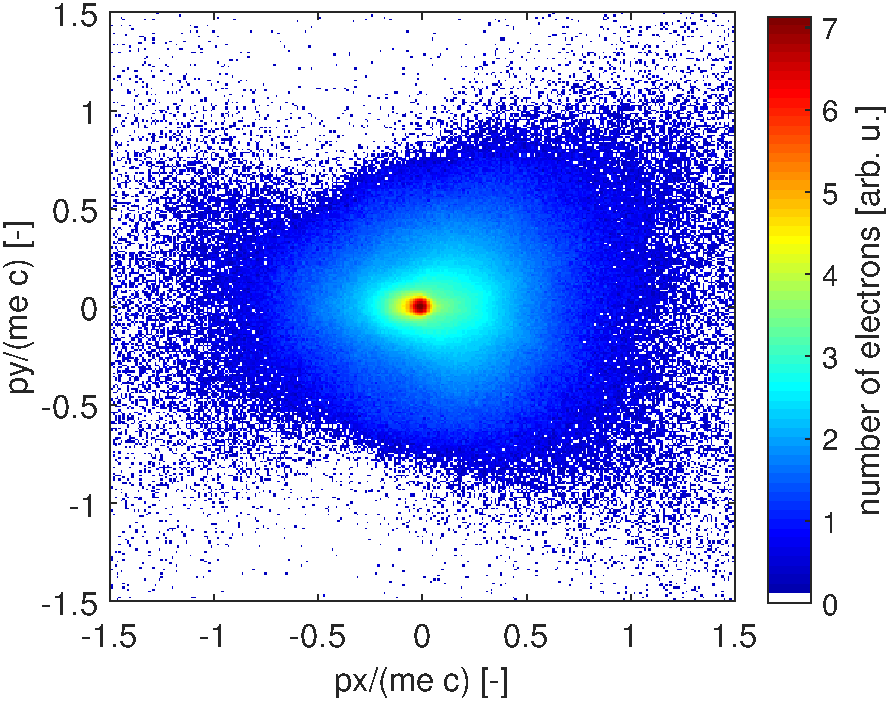
\includegraphics[width=0.45\linewidth]{./img/results/i1e20/05/px_py.pdf}}}
	\sidesubfloat[]{{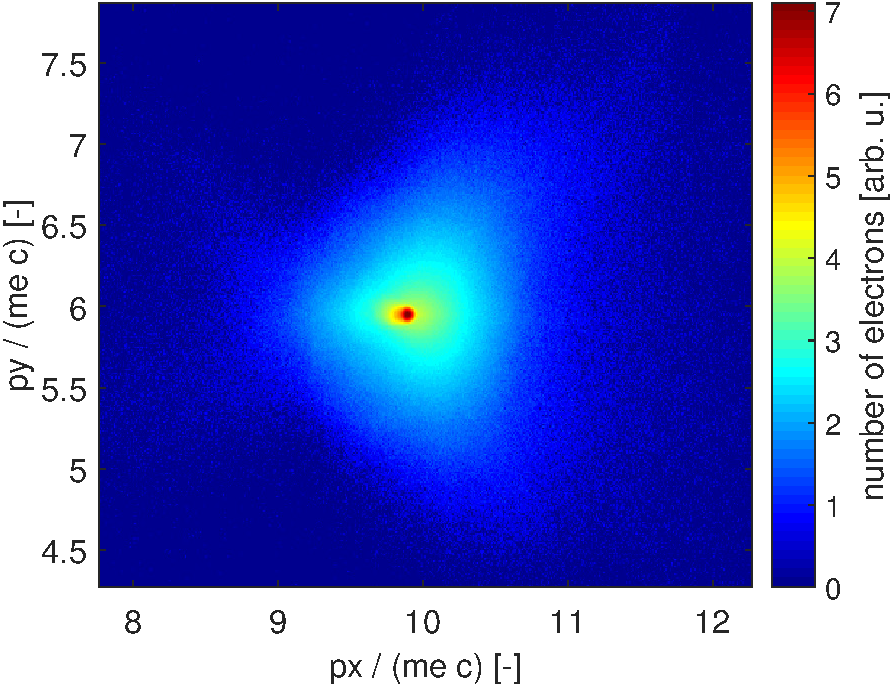
\includegraphics[width=0.45\linewidth]{./img/results/i1e20/2/px_py.pdf}}}\\
	\sidesubfloat[]{{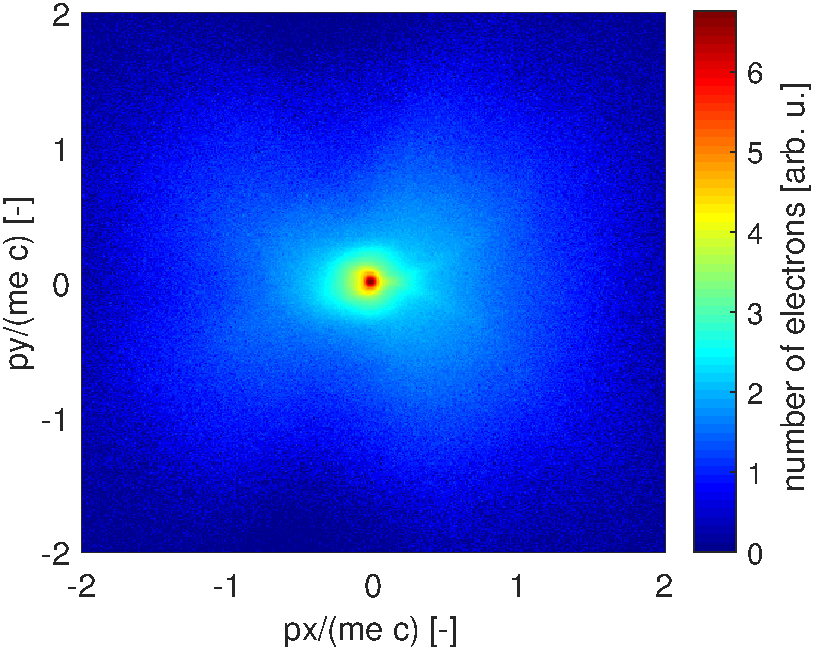
\includegraphics[width=0.45\linewidth]{./img/results/i1e21/05/px_py.pdf}}}
	\sidesubfloat[]{{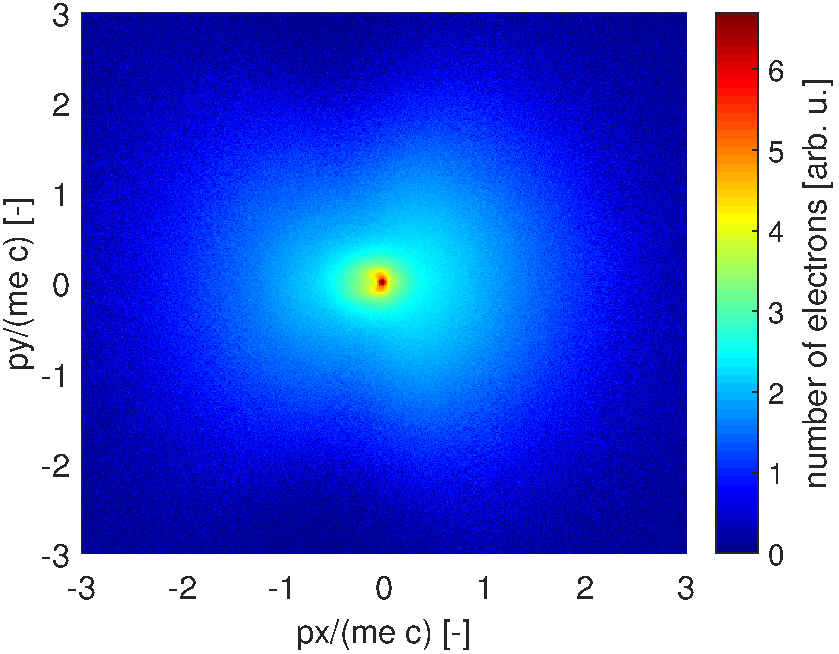
\includegraphics[width=0.45\linewidth]{./img/results/i1e21/2/px_py.pdf}}}
	\caption{\textbf{(a)} w0 = 05 micron, I = 1e20 W/cm2, t = 100 fs \textbf{(b)} w0 = 2 micron, I = 1e20 W/cm2, t = 100 fs \textbf{(c)} w0 = 05 micron, I = 1e21 W/cm2, t = 100 fs \textbf{(d)} w0 = 2 micron, I = 1e21 W/cm2, t = 100 fs}
	\label{}
\end{figure}

\floatsetup[figure]{style=plain, subcapbesideposition=top}
\begin{figure}[h!]
	\centering
	\sidesubfloat[]{{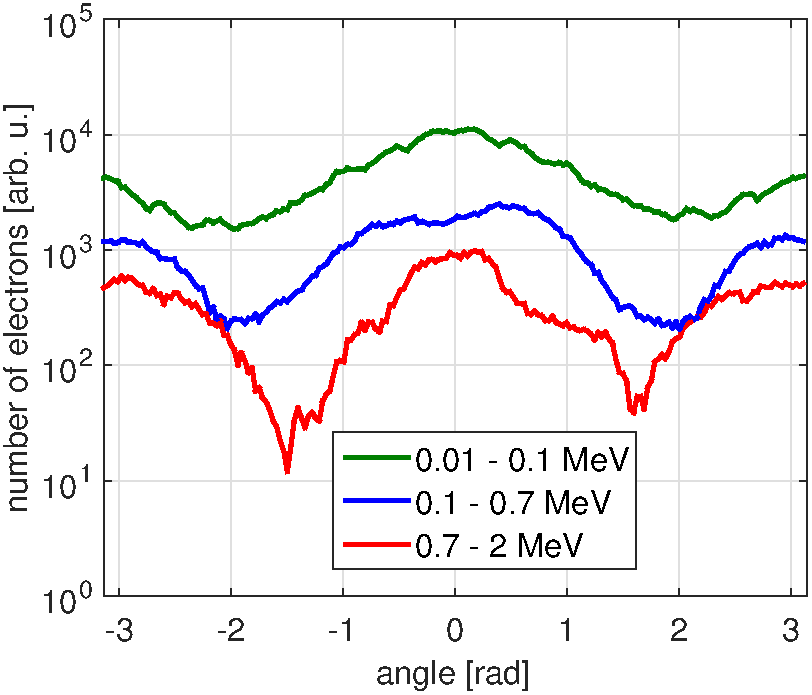
\includegraphics[width=0.445\linewidth]{./img/results/i1e20/05/angles.pdf}}}
	\hspace{1mm}
	\sidesubfloat[]{{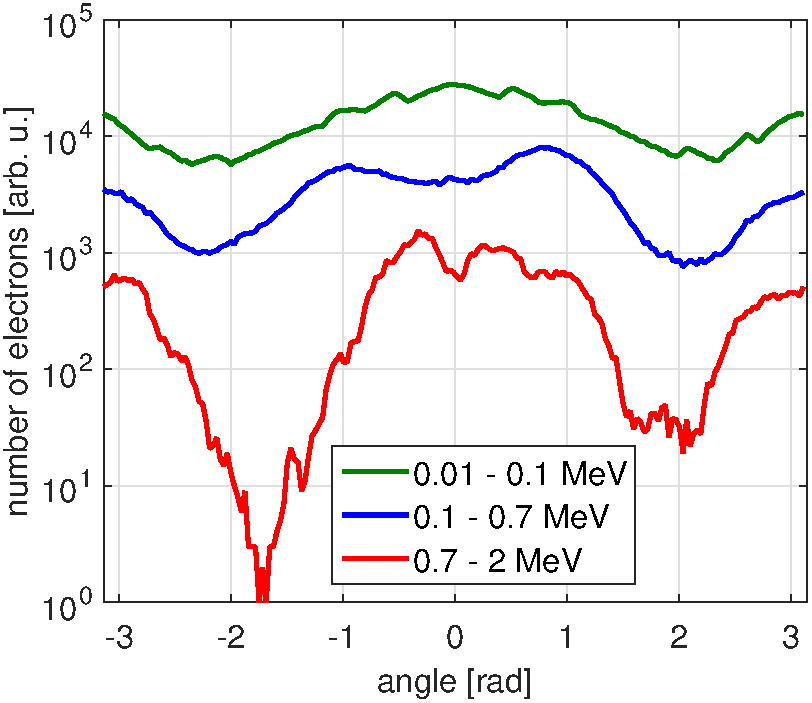
\includegraphics[width=0.445\linewidth]{./img/results/i1e20/2/angles.pdf}}}\\
	\sidesubfloat[]{{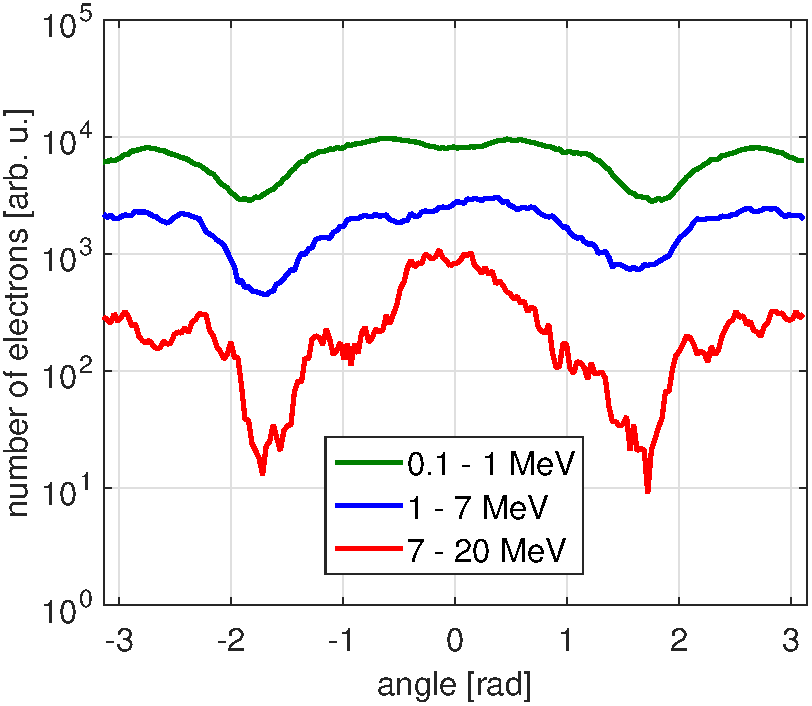
\includegraphics[width=0.445\linewidth]{./img/results/i1e21/05/angles.pdf}}}
	\hspace{1mm}
	\sidesubfloat[]{{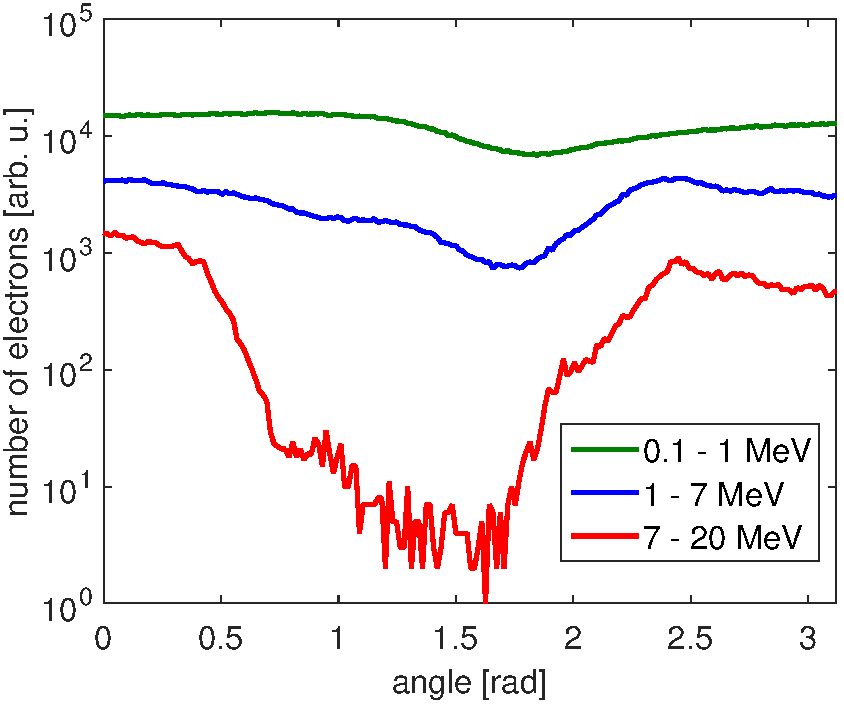
\includegraphics[width=0.445\linewidth]{./img/results/i1e21/2/angles.pdf}}}
	\caption{}
	\label{}
\end{figure}

\floatsetup[figure]{style=plain, subcapbesideposition=top}
\begin{figure}[h!]
	\centering
	\sidesubfloat[]{{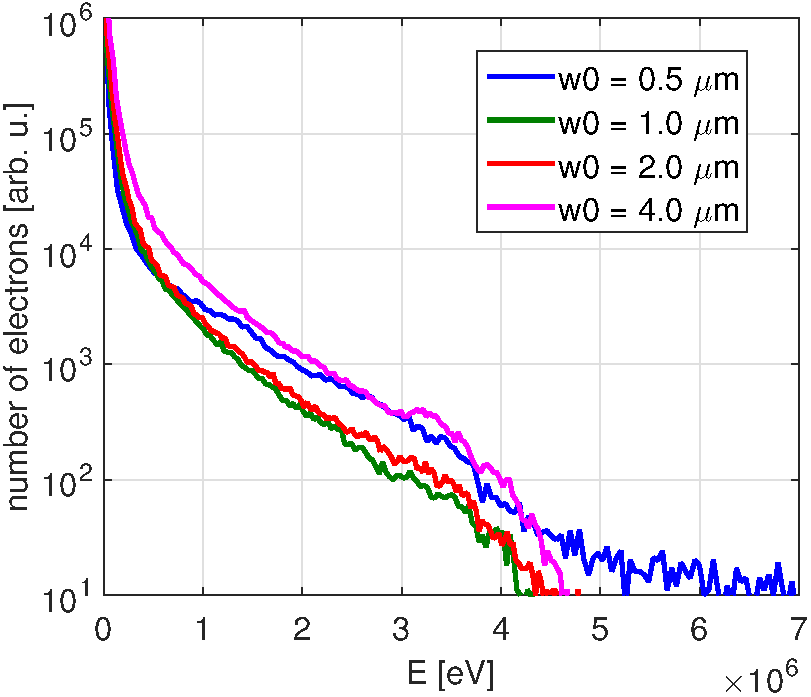
\includegraphics[width=0.445\linewidth]{./img/results/i1e20/dist_e.pdf}}}
	\hspace{1mm}
	\sidesubfloat[]{{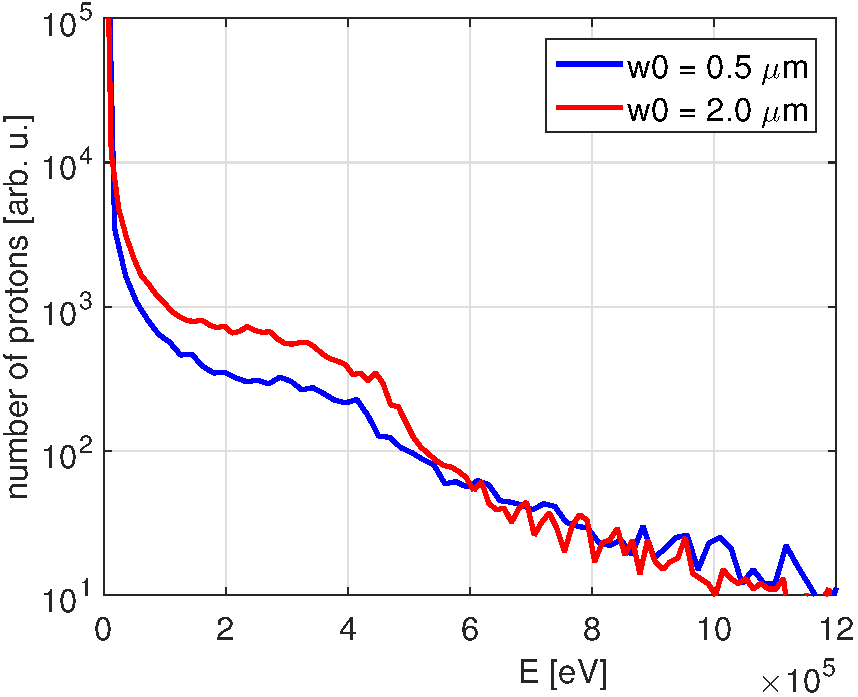
\includegraphics[width=0.445\linewidth]{./img/results/i1e20/dist_p.pdf}}}\\[2mm]
	\sidesubfloat[]{{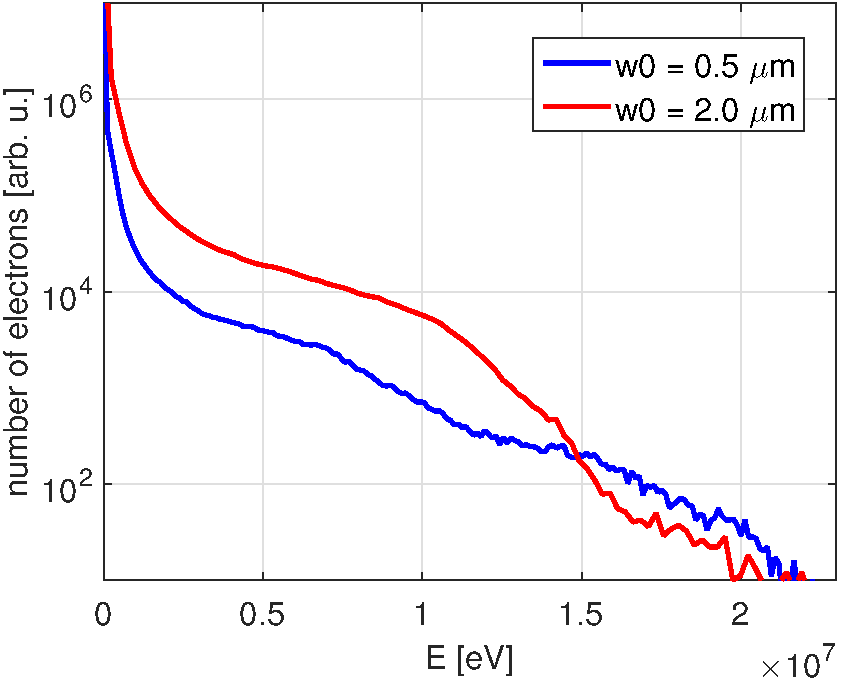
\includegraphics[width=0.445\linewidth]{./img/results/i1e21/dist_e.pdf}}}
	\hspace{1mm}
	\sidesubfloat[]{{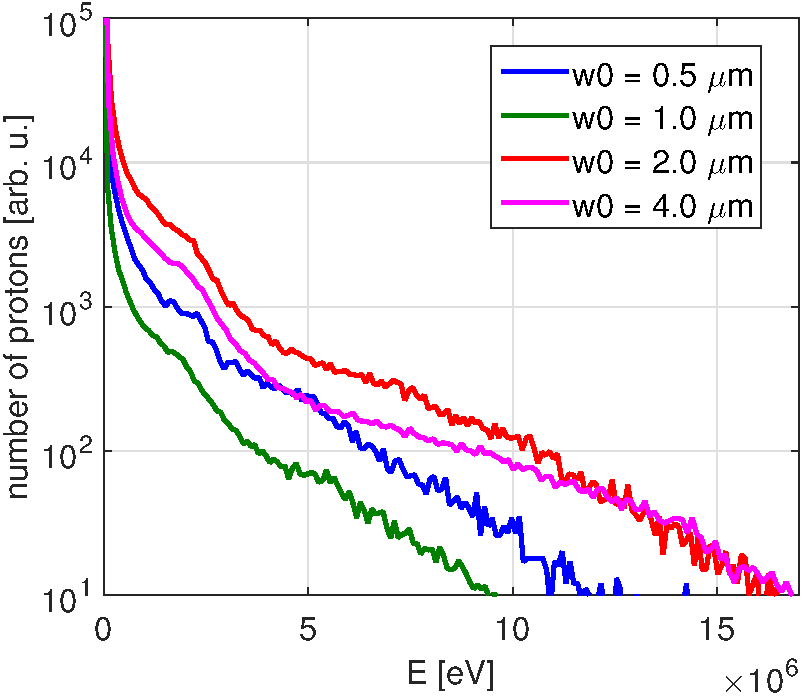
\includegraphics[width=0.445\linewidth]{./img/results/i1e21/dist_p.pdf}}}
	\caption{}
	\label{}
\end{figure}

\floatsetup[figure]{style=plain, subcapbesideposition=top}
\begin{figure}[h!]
	\centering
	\sidesubfloat[]{{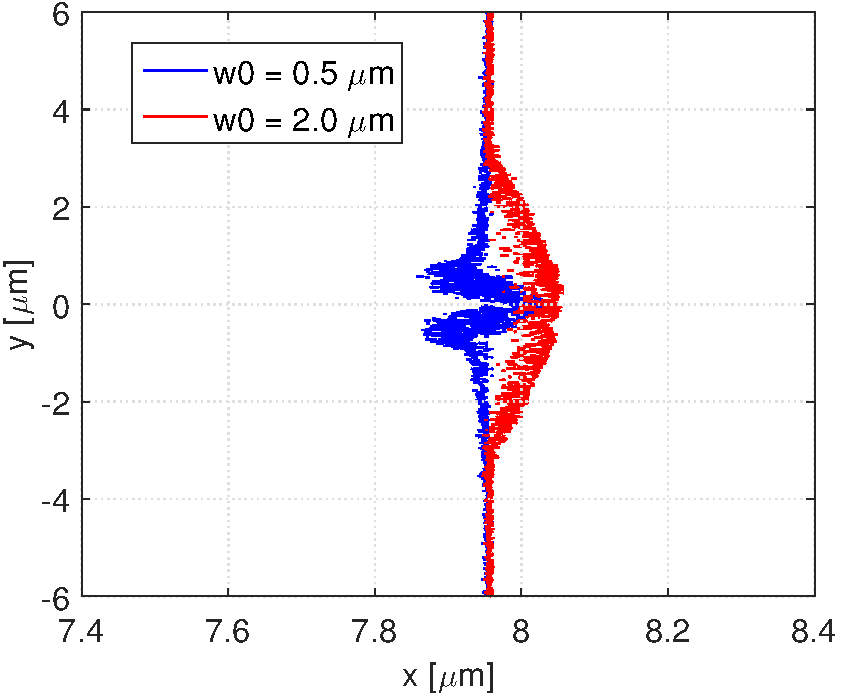
\includegraphics[width=0.445\linewidth]{./img/results/i1e20/dens.pdf}}}
	\hspace{1mm}
	\sidesubfloat[]{{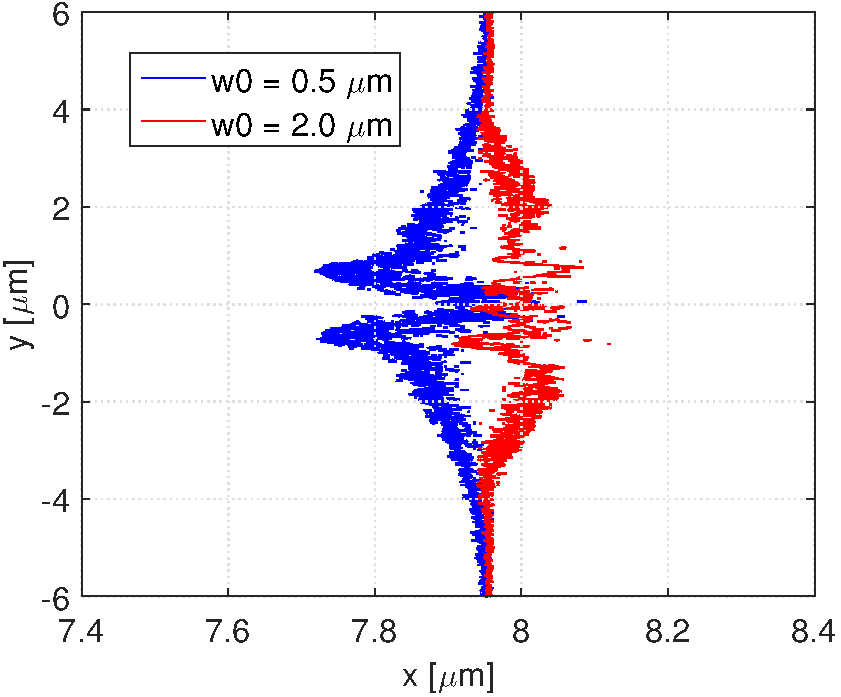
\includegraphics[width=0.445\linewidth]{./img/results/i1e21/dens.pdf}}}
	\caption{\textbf{(a)} nc protons, t = 100 fs, I = 1e20 W/cm2 \textbf{(b)} nc protons, t = 100 fs, I = 1e21 W/cm2}
	\label{}
\end{figure}

\floatsetup[figure]{style=plain, subcapbesideposition=top}
\begin{figure}[h!]
	\centering
	\sidesubfloat[]{{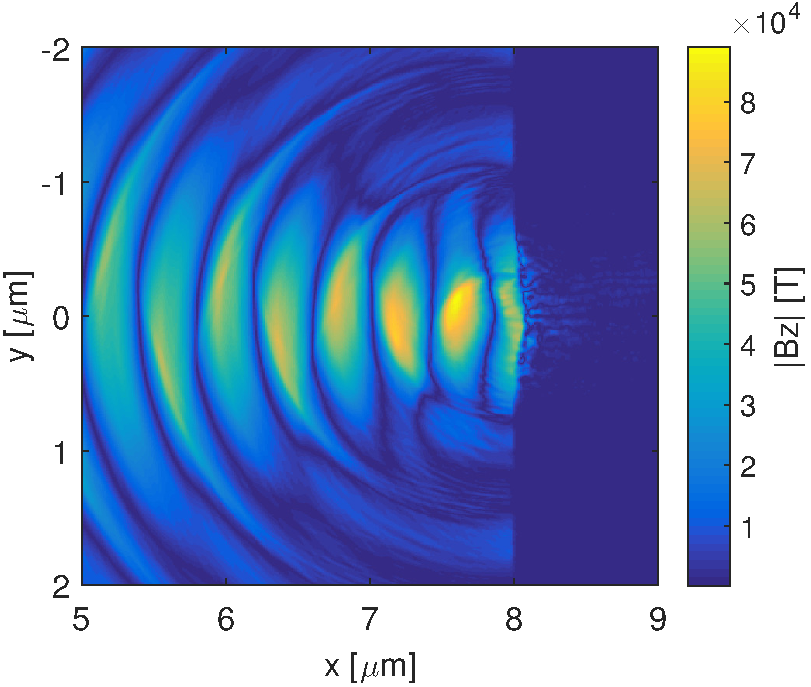
\includegraphics[width=0.45\linewidth]{./img/results/i1e20/05/abs_Bz.pdf}}}
	\sidesubfloat[]{{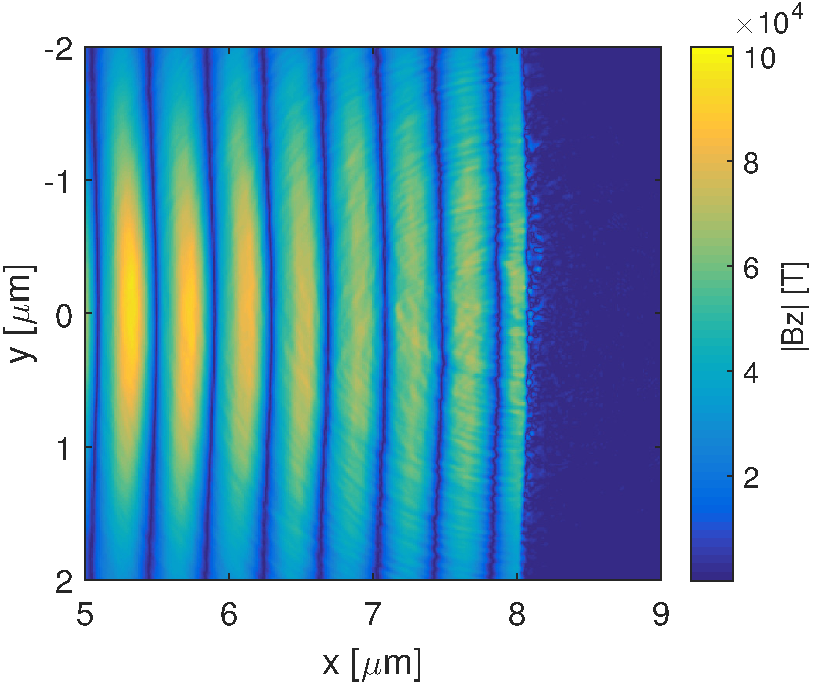
\includegraphics[width=0.45\linewidth]{./img/results/i1e20/2/abs_Bz.pdf}}}\\[2mm]
	\sidesubfloat[]{{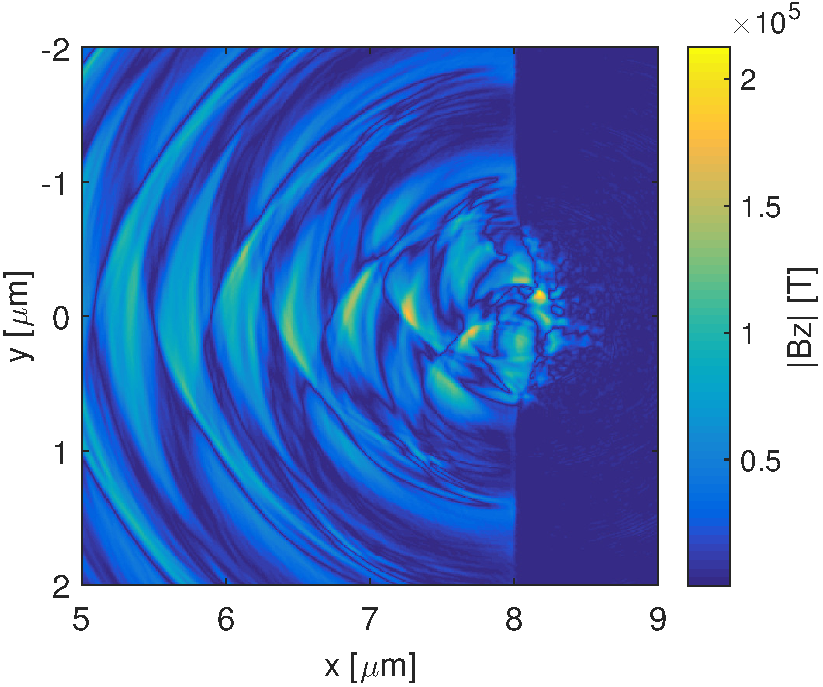
\includegraphics[width=0.45\linewidth]{./img/results/i1e21/05/abs_Bz.pdf}}}
	\sidesubfloat[]{{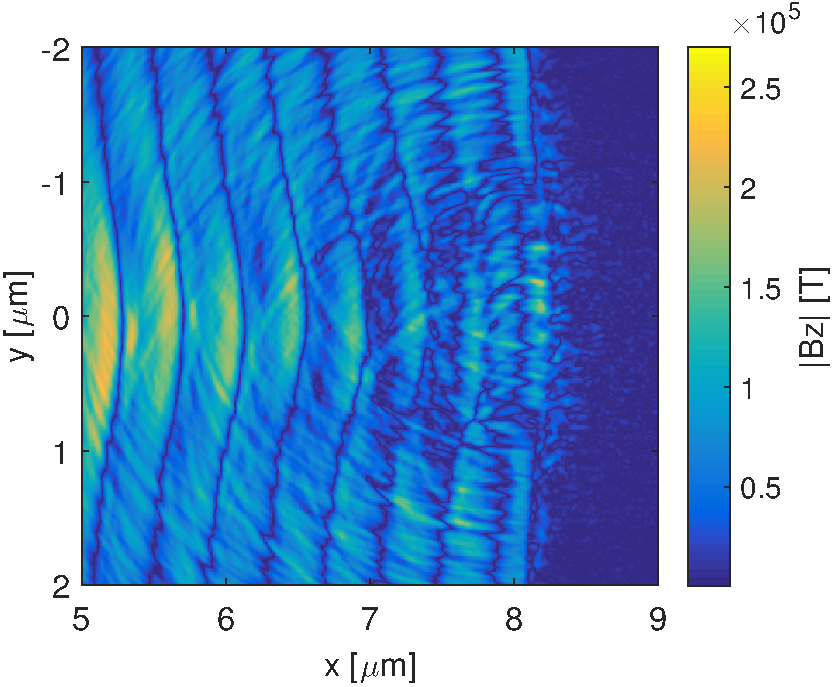
\includegraphics[width=0.45\linewidth]{./img/results/i1e21/2/abs_Bz.pdf}}}
	\caption{}
	\label{}
\end{figure}

\floatsetup[figure]{style=plain, subcapbesideposition=top}
\begin{figure}[h!]
	\centering
	\sidesubfloat[]{{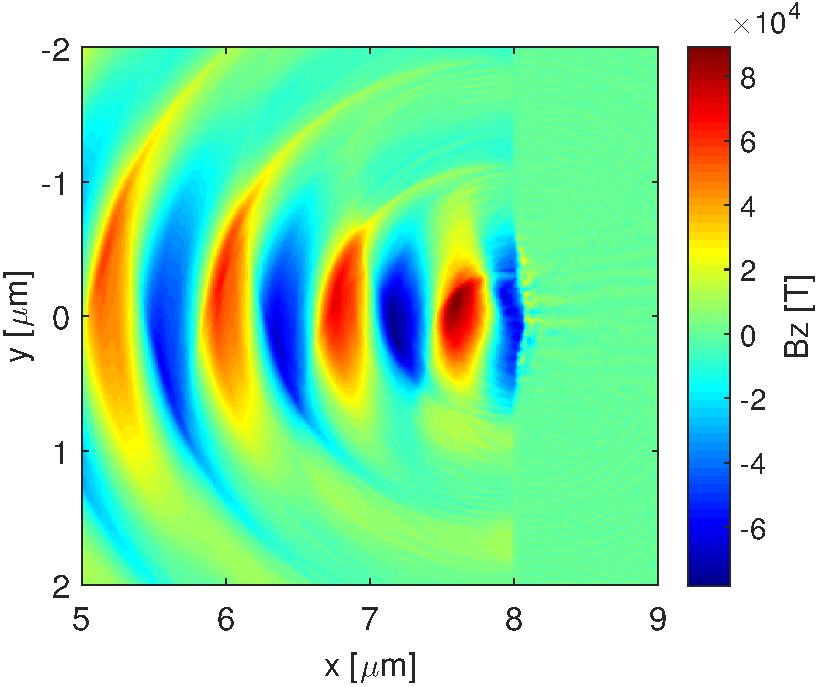
\includegraphics[width=0.45\linewidth]{./img/results/i1e20/05/Bz.pdf}}}
	\sidesubfloat[]{{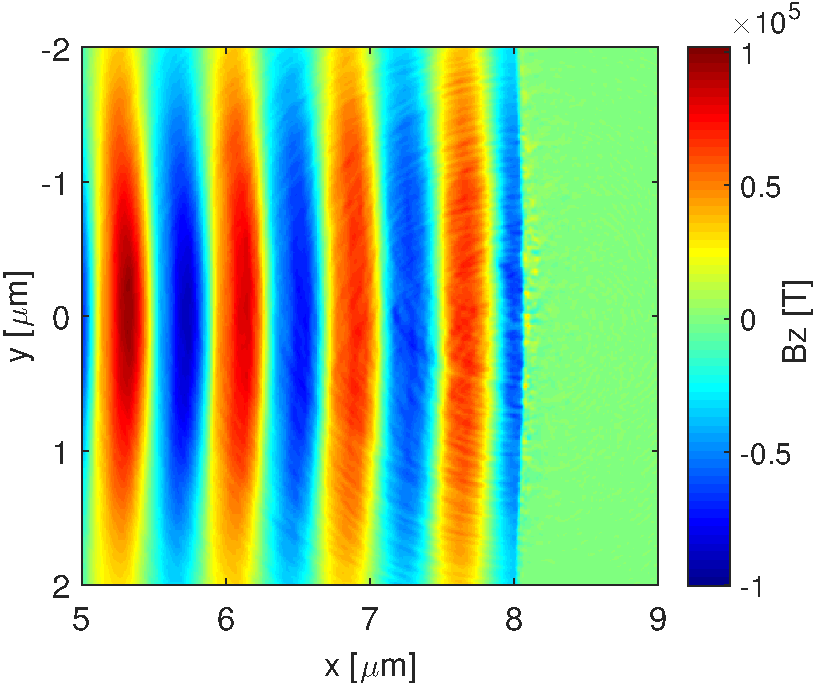
\includegraphics[width=0.45\linewidth]{./img/results/i1e20/2/Bz.pdf}}}\\[2mm]
	\sidesubfloat[]{{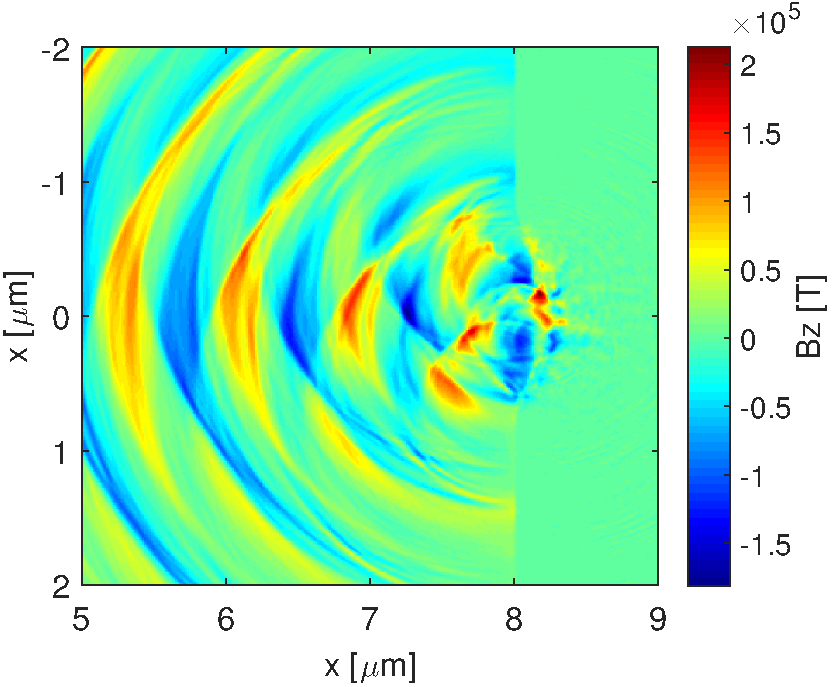
\includegraphics[width=0.45\linewidth]{./img/results/i1e21/05/Bz.pdf}}}
	\sidesubfloat[]{{\includegraphics[width=0.45\linewidth]{./img/results/i1e21/2/Bz.pdf}}}
	\caption{}
	\label{}
\end{figure}

\floatsetup[figure]{style=plain, subcapbesideposition=top}
\begin{figure}[h!]
	\centering
	\sidesubfloat[]{{\includegraphics[width=0.445\linewidth]{./img/results/i1e21/05/trajectories.pdf}}}
	\hspace{1mm}
	\sidesubfloat[]{{\includegraphics[width=0.445\linewidth]{./img/results/i1e21/2/trajectories.pdf}}}
	\caption{\textbf{(a)} electrons, w0 = 0.5 micron, t = 100 fs, I = 1e21 W/cm2 \textbf{(b)} electrons, wo = 2 micron, t = 100 fs, I = 1e21 W/cm2}
	\label{}
\end{figure}

\floatsetup[figure]{style=plain, subcapbesideposition=top}
\begin{figure}[h!]
	\centering
	\sidesubfloat[]{{\includegraphics[width=0.45\linewidth]{./img/results/i1e20/05/abs_Fpx.pdf}}}
	\sidesubfloat[]{{\includegraphics[width=0.45\linewidth]{./img/results/i1e20/05/abs_Ex.pdf}}}\\
	\sidesubfloat[]{{\includegraphics[width=0.45\linewidth]{./img/results/i1e20/2/abs_Fpx.pdf}}}
	\sidesubfloat[]{{\includegraphics[width=0.45\linewidth]{./img/results/i1e20/2/abs_Ex.pdf}}}
	\caption{}
	\label{}
\end{figure}

\floatsetup[figure]{style=plain, subcapbesideposition=top}
\begin{figure}[h!]
	\centering
	\sidesubfloat[]{{\includegraphics[width=0.45\linewidth]{./img/results/i1e21/05/abs_Fpx.pdf}}}
	\sidesubfloat[]{{\includegraphics[width=0.45\linewidth]{./img/results/i1e21/05/abs_Ex.pdf}}}\\
	\sidesubfloat[]{{\includegraphics[width=0.45\linewidth]{./img/results/i1e21/2/abs_Fpx.pdf}}}
	\sidesubfloat[]{{\includegraphics[width=0.45\linewidth]{./img/results/i1e21/2/abs_Ex.pdf}}}
	\caption{}
	\label{}
\end{figure}

%-------------------------------------------------------------------------------

%\noindent
Zeroth set (4 simulations with const. E = 2.8306e4 J, traget 2 micron, 2000 ppc):
\noindent
Laser:
\begin{itemize}
	\item wavelength: $ \lambda $ = 0.8 $ \mu m $
	\item const. energy: E = 2.8306e4 J (corresponds to I = 1e20 W/cm2 for $ w_0 $ = 1.0 $ \mu m $)
	\item duration: t = 30 fs (in FWHM)
	\item beam waist in focus: $ w_0 $ = 0.5, 1.0, 2.0, 4.0 $ \mu m $
	\item focus distance from boundary: $ x_\mathrm{B} - x_0 $ = 8 $ \mu m $
	\item polarization: P
	\item boundary: left 
\end{itemize}
Domain:
\begin{itemize}
	\item x min: 0 $ \mu m $
	\item x max: 15 $ \mu m $
	\item y min: -20 $ \mu m $
	\item y max: 20 $ \mu m $
	\item $ N_x $: 1875 cells ($ \delta x $ = $ \lambda/100 $ = 8 nm)
	\item $ N_y $: 5000 cells ($ \delta y $ = $ \lambda/100 $ = 8 nm)
	\item time step: $ \delta t $ = $ 1/(\sqrt{2} c) \lambda /100 \approx $ 0.05 fs 
	\item simulation time: $ \tau $ = 200 fs
\end{itemize}
Target:
\begin{itemize}
	\item x min: 8 $ \mu m $
	\item x max: 10 $ \mu m $
	\item y min: -15 $ \mu m $
	\item y max: 15 $ \mu m $
	\item electrons: 2000 ppc
	\item protons: 100 ppc
	\item density: 100 critical
	\item temperature: 100 eV
\end{itemize}

\noindent
First set (4 simulations with const. I = 1e20 W/cm2, traget 2 micron, 2000 ppc):
\noindent
Laser:
\begin{itemize}
	\item wavelength: $ \lambda $ = 0.8 $ \mu m $
	\item const. intensity: I = 1e20 W/cm2
	\item duration: t = 30 fs (in FWHM)
	\item beam waist in focus: $ w_0 $ = 0.5, 1.0, 2.0, 4.0 $ \mu m $
	\item focus distance from boundary: $ x_\mathrm{B} - x_0 $ = 8 $ \mu m $
	\item polarization: P
	\item boundary: left 
\end{itemize}
Domain:
\begin{itemize}
	\item x min: 0 $ \mu m $
	\item x max: 15 $ \mu m $
	\item y min: -20 $ \mu m $
	\item y max: 20 $ \mu m $
	\item $ N_x $: 1875 cells ($ \delta x $ = $ \lambda/100 $ = 8 nm)
	\item $ N_y $: 5000 cells ($ \delta y $ = $ \lambda/100 $ = 8 nm)
	\item time step: $ \delta t $ = $ 1/(\sqrt{2} c) \lambda /100 \approx $ 0.05 fs 
	\item simulation time: $ \tau $ = 200 fs
\end{itemize}
Target:
\begin{itemize}
	\item x min: 8 $ \mu m $
	\item x max: 10 $ \mu m $
	\item y min: -15 $ \mu m $
	\item y max: 15 $ \mu m $
	\item electrons: 2000 ppc
	\item protons: 100 ppc
	\item density: 100 critical
	\item temperature: 100 eV
\end{itemize}

\noindent
Seconds set (4 simulations with const. I = 1e21, 1000 ppc):
\noindent
Laser:
\begin{itemize}
	\item wavelength: $ \lambda $ = 0.8 $ \mu m $
	\item const intensity: I = 1e21 W/cm2
	\item duration: t = 30 fs (in FWHM)
	\item beam waist in focus: $ w_0 $ = 0.5, 1.0, 2.0, 4.0 $ \mu m $
	\item focus distance from boundary: $ x_\mathrm{B} - x_0 $ = 8 $ \mu m $
	\item polarization: P
	\item boundary: left 
\end{itemize}
Domain:
\begin{itemize}
	\item x min: 0 $ \mu m $
	\item x max: 15 $ \mu m $
	\item y min: -20 $ \mu m $
	\item y max: 20 $ \mu m $
	\item $ N_x $: 1875 cells ($ \delta x $ = $ \lambda/100 $ = 8 nm)
	\item $ N_y $: 5000 cells ($ \delta y $ = $ \lambda/100 $ = 8 nm)
	\item time step: $ \delta t $ = $ 1/(\sqrt{2} c) \lambda /100 \approx $ 0.05 fs 
	\item simulation time: $ \tau $ = 200 fs
\end{itemize}
Target:
\begin{itemize}
	\item x min: 8 $ \mu m $
	\item x max: 10 $ \mu m $
	\item y min: -15 $ \mu m $
	\item y max: 15 $ \mu m $
	\item electrons: 1000 ppc
	\item protons: 100 ppc
	\item density: 100 critical
	\item temperature: 100 eV
\end{itemize}

\noindent
Third set (2 simulations with I = 1e21 W/cm2, thiner target (0.25 micron), 2000 ppc):
\noindent
Laser:
\begin{itemize}
	\item wavelength: $ \lambda $ = 0.8 $ \mu m $
	\item const intensity: I = 1e21 W/cm2
	\item duration: t = 30 fs (in FWHM)
	\item beam waist in focus: $ w_0 $ = 0.5, 2.0 $ \mu m $
	\item focus distance from boundary: $ x_\mathrm{B} - x_0 $ = 8 $ \mu m $
	\item polarization: P
	\item boundary: left 
\end{itemize}
Domain:
\begin{itemize}
	\item x min: 0 $ \mu m $
	\item x max: 15 $ \mu m $
	\item y min: -20 $ \mu m $
	\item y max: 20 $ \mu m $
	\item $ N_x $: 1875 cells ($ \delta x $ = $ \lambda/100 $ = 8 nm)
	\item $ N_y $: 5000 cells ($ \delta y $ = $ \lambda/100 $ = 8 nm)
	\item time step: $ \delta t $ = $ 1/(\sqrt{2} c) \lambda /100 \approx $ 0.05 fs 
	\item simulation time: $ \tau $ = 200 fs
\end{itemize}
Target:
\begin{itemize}
	\item x min: 8 $ \mu m $
	\item x max: 8.25 $ \mu m $
	\item y min: -15 $ \mu m $
	\item y max: 15 $ \mu m $
	\item electrons: 2000 ppc
	\item protons: 100 ppc
	\item density: 100 critical
	\item temperature: 100 eV
\end{itemize}
%\newpage
\noindent
$ \vec{E} $ and $ \vec{B} $ fields in terms of scalar potential $ \Phi $ and vector potential $ \vec{A} $:
\begin{equation*}
	\vec{E} = - \grad{\Phi} - \diffp{\vec{A}}{t}, \qquad \vec{B} = \rot{\vec{A}}
\end{equation*}
$ \Phi $ and $ \vec{A} $ in the form of plane waves propagating along z-axis:
\begin{equation*}
	\vec{A}\left(x, y, z, t\right)  = \vec{A_0}\left( x, y, z\right) \e^{i(k_z z - \omega t)}, \qquad \Phi\left(x, y, z, t \right) = \Phi_0\left(x, y, z\right) \e^{i(k_z z - \omega t)}
\end{equation*}
Lorentz gauge condition:
\begin{equation*}
	\div{\vec{A}} + \frac{1}{c^2} \diffp{\Phi}{t} = 0
\end{equation*}
scalar potential in terms of vector potential:
\begin{equation*}
	\diffp{\Phi}{t} = - \i \omega \Phi \qquad \longrightarrow \qquad \Phi = - \i \frac{c}{k_z} \div{\vec{A}} 
\end{equation*}
$ \vec{E} $ and $ \vec{B} $ fields in terms of vector potential $ \vec{A} $:
\begin{equation*}
	\vec{E} = \i \frac{c}{k_z} \grad{\left(\div{\vec{A}}\right)} + \i \omega \vec{A}, \qquad \vec{B} = \rot{\vec{A}}
\end{equation*}
wave equation for vector potential $ \vec{A} $:
\begin{equation*}
\laplace{\vec{A}} - \frac{1}{c^2}\diffp[2]{\vec{A}}{t} = 0
\end{equation*}
Helmholtz equation:
\begin{equation*}
\laplace{\vec{A_0}} + 2 \i k_z \diffp{\vec{A_0}}{z} = 0
\end{equation*}
paraxial (slowly varying envelope) approximation:
\begin{equation*}
\left\| \diffp[2]{\vec{A_0}}{z}\right\|  \leq \left\|2 k_z \diffp{\vec{A_0}}{z}\right\|  \longrightarrow 
\diffp[2]{\vec{A_0}}{x} + \diffp[2]{\vec{A_0}}{y} + \diffp[2]{\vec{A_0}}{z} + 2 \i k_z \diffp{\vec{A_0}}{z} = 0
\end{equation*}
\newpage
\noindent
Solution - Gaussian beam:
\begin{equation*}
\vec{E}\left(x, y, z \right) = \vec{E_0} \frac{w_0}{w(z)} \exp \left( - \frac{x^2 + y^2}{w(z)^2} \right) \cos\left( \omega t - k_z \left(z + \frac{x^2 + y^2}{2R(z)} \right) + \phi_G(z) \right) 
\end{equation*}
where
\begin{flalign*}
& w(z) = w_0 \sqrt{1 + \left(\frac{z}{z_R} \right)^2} \dots \mathrm{evolving \: beam \: width} & \\
& z_r = \frac{\pi w_0^2}{\lambda} \dots \mathrm{Rayleigh \: range} & \\
& R(z) = z\left(1 + \left(\frac{z_R}{z} \right)^2 \right) \dots \mathrm{evolving \: radius \: of \: curvature} & \\
& \phi(z) = \tan^{-1}\left(\frac{z}{z_R} \right) \dots \mathrm{Guoy \: phase} & \\
& \theta = \tan^{-1}\left(\frac{w(z)}{z} \right) \simeq \frac{\lambda}{\pi w_0} \dots \mathrm{beam \: divergence \: angle} &
\end{flalign*}

\noindent
Features:
\begin{itemize}
	\item 2D version of algorithm, Ey, Bx, Bz omitted (identically equal to 0) 
	\item Code written in C++, object oriented to be easily extended to 3D, compiled to static library
	\item Linked into EPOCH as a static library (in order not to disturb the code, for this reason also added support for CMake – machine independent)
	\item Parallelized using hybrid techniques (OpenMP + MPI – computation time in most cases negligible in comparison with the main simulation)
	\item Fourier transforms can be computed using Intel MKL library, FFTW library or without any library (compile time option)
	\item Computed fields dumped into shared files using binary coding (speed up output, save disk storage)
	\item Only transverse component of electric field (Ex) passed to the EPOCH at each time step (no significant slowdown or memory overhead), other fields computed by EPOCH
	\item All new parameters needed for tight-focusing (w0, focal length, etc.) may be specified via input file
	\item Implementation works generally regardless the number of lasers in the simulation or boundaries that they are attached to
\end{itemize}

\begin{lstlisting}[style=CXX, caption=Function performing forward fast Fourier transform using MKL library]
std::vector<std::complex<double>> fft::mkl_fft_forward(std::vector<std::complex<double>> in) {
DFTI_DESCRIPTOR_HANDLE desc;
MKL_LONG status;
DftiCreateDescriptor(&desc, DFTI_DOUBLE, DFTI_COMPLEX, 1, static_cast<MKL_LONG>(in.size()));
DftiCommitDescriptor(desc);
status = DftiComputeForward(desc, in.data());
if(status != 0) {
std::cerr << DftiErrorMessage(status) << std::endl;
abort();
}
DftiFreeDescriptor(&desc);
return in;
}
\end{lstlisting}

\begin{lstlisting}[style=CXX, caption=Function performing backward fast Fourier transform using MKL library]
std::vector<std::complex<double>> fft::mkl_fft_backward(std::vector<std::complex<double>> in) {
DFTI_DESCRIPTOR_HANDLE desc;
MKL_LONG status;
DftiCreateDescriptor(&desc, DFTI_DOUBLE, DFTI_COMPLEX, 1, static_cast<MKL_LONG>(in.size()));
DftiCommitDescriptor(desc);
status = DftiComputeBackward(desc, in.data());
if(status != 0) {
std::cerr << DftiErrorMessage(status) << std::endl;
abort();
}
DftiFreeDescriptor(&desc);
return in;
}
\end{lstlisting}

\begin{lstlisting}[style=CXX, caption=Function performing forward fast Fourier transform using FFTW library]
std::vector<std::complex<double>> fft::fftw_fft_forward(std::vector<std::complex<double>> in) {
fftw_plan p = fftw_plan_dft_1d(in.size(), reinterpret_cast<fftw_complex*>(in.data()), reinterpret_cast<fftw_complex*>(in.data()), FFTW_FORWARD, FFTW_ESTIMATE);
fftw_execute(p);
fftw_destroy_plan(p);
return in;
}
\end{lstlisting}

\begin{lstlisting}[style=CXX, caption=Function performing backward fast Fourier transform using FFTW library]
std::vector<std::complex<double>> fft::fftw_fft_backward(std::vector<std::complex<double>> in) {
fftw_plan p = fftw_plan_dft_1d(in.size(), reinterpret_cast<fftw_complex*>(in.data()), reinterpret_cast<fftw_complex*>(in.data()), FFTW_BACKWARD, FFTW_ESTIMATE);
fftw_execute(p);
fftw_destroy_plan(p);
return in;
}
\end{lstlisting}

\begin{lstlisting}[style=CXX, caption=Function performing forward discrete Fourier transform without using any library]
std::vector<std::complex<double>> fft::fft_forward(std::vector<std::complex<double>> in) {
std::vector<std::complex<double>> out(in.size());
for(auto j = 0; j < out.size(); j++) {
for(auto l = 0; l < out.size(); l++) {
out.at(j) += in.at(l) * exp(-2.0 * constants::pi * I * l * j / in.size());
}
}
return out;
}
\end{lstlisting}

\begin{lstlisting}[style=CXX, caption=Function performing backward discrete Fourier transform without using any library]
std::vector<std::complex<double>> fft::fft_backward(std::vector<std::complex<double>> in) {
std::vector<std::complex<double>> out(in.size());
for(auto j = 0; j < out.size(); j++) {
for(auto l = 0; l < out.size(); l++) {
out.at(j) += in.at(l) * exp(+2.0 * constants::pi * I * l * j / in.size());
}
}
return out;
}
\end{lstlisting}

\begin{lstlisting}[style=CXX, caption=Method for performing discrete Fourier transform in time]
void laser_bcs::dft_time(field_2d<std::complex<double>>& field) const {
#ifdef OPENMP
#pragma omp parallel for schedule(static)
#endif
for(auto j = 0; j < this->domain->Nx; j++) {
#ifdef USE_MKL
field.add_col(fft::mkl_fft_backward(field.get_col(j)), j);
#elif USE_FFTW
field.add_col(fft::fftw_fft_backward(field.get_col(j)), j);
#else
field.add_col(fft::fft_backward(field.get_col(j)), j);
#endif
}
field.multiply(this->domain->dt / (2.0 * constants::pi));
return;
}
\end{lstlisting}

\begin{lstlisting}[style=CXX, caption=Method for performing inverse discrete Fourier transform in time]
void laser_bcs::idft_time(field_2d<std::complex<double>>& field) const {
#ifdef OPENMP
#pragma omp parallel for schedule(static)
#endif
for(auto j = 0; j < this->domain->Nx; j++) {
#ifdef USE_MKL
field.add_col(fft::mkl_fft_forward(field.get_col(j)), j);
#elif USE_FFTW
field.add_col(fft::fftw_fft_forward(field.get_col(j)), j);
#else
field.add_col(fft::fft_forward(field.get_col(j)), j);
#endif
}
field.multiply(2.0 * (2.0 * constants::pi) / (this->domain->Nt * this->domain->dt));
return;
}
\end{lstlisting}

\begin{lstlisting}[style=CXX, caption=Method for performing discrete Fourier transform in space]
void laser_bcs::dft_space(field_2d<std::complex<double>>& field) const {
std::vector<std::complex<double>> row_global(this->domain->Nx_global);
std::vector<std::complex<double>> row_local;
for(auto j = 0; j < this->domain->Nt; j++) {
row_local = field.get_row(j);
MPI_Gatherv(row_local.data(), this->domain->Nx, MPI_CXX_DOUBLE_COMPLEX, row_global.data(), this->domain->counts.data(), this->domain->displs.data(), MPI_CXX_DOUBLE_COMPLEX, 0, MPI_COMM_WORLD);
if(this->domain->rank == 0) {
#ifdef USE_MKL
row_global = fft::mkl_fft_forward(row_global);
#elif USE_FFTW
row_global = fft::fftw_fft_forward(row_global);
#else
row_global = fft::fft_forward(row_global);
#endif
}
MPI_Scatterv(row_global.data(), this->domain->counts.data(), this->domain->displs.data(), 	MPI_CXX_DOUBLE_COMPLEX, row_local.data(), this->domain->Nx, MPI_CXX_DOUBLE_COMPLEX, 0, MPI_COMM_WORLD);
field.add_row(row_local, j);
}
field.multiply(this->domain->dx / (2.0 * constants::pi));
return;
}
\end{lstlisting}

\begin{lstlisting}[style=CXX, caption=Method for performing inverse discrete Fourier transform in space]
void laser_bcs::idft_space(field_2d<std::complex<double>>& field) const {
std::vector<std::complex<double>> row_global(this->domain->Nx_global);
std::vector<std::complex<double>> row_local;
for(auto j = 0; j < this->domain->Nt; j++) {
row_local = field.get_row(j);
MPI_Gatherv(row_local.data(), this->domain->Nx, MPI_CXX_DOUBLE_COMPLEX, row_global.data(), this->domain->counts.data(), this->domain->displs.data(), MPI_CXX_DOUBLE_COMPLEX, 0, MPI_COMM_WORLD);
if(this->domain->rank == 0) {
#ifdef USE_MKL
row_global = fft::mkl_fft_backward(row_global);
#elif USE_FFTW
row_global = fft::fftw_fft_backward(row_global);
#else
row_global = fft::fft_backward(row_global);
#endif
}
MPI_Scatterv(row_global.data(), this->domain->counts.data(), this->domain->displs.data(), MPI_CXX_DOUBLE_COMPLEX, row_local.data(), this->domain->Nx, MPI_CXX_DOUBLE_COMPLEX, 0, MPI_COMM_WORLD);
field.add_row(row_local, j);
}
field.multiply((2.0 * constants::pi) / (this->domain->Nx_global * this->domain->dx));
return;
}
\end{lstlisting}

\begin{lstlisting}[style=CXX, caption=Method for dumping data into shared file]
template <typename T>
void field_2d<T>::dump_to_shared_file(std::string name, int row_first, int row_last, int row_size_local, int row_size_global, int col_start) const {
MPI_File file;
MPI_Offset offset = 0;
MPI_Status status;
MPI_Datatype local_array;
int col_size = row_last - row_first;
const int ndims = 2;
std::array<int, ndims> size_global = {col_size, row_size_global};
std::array<int, ndims> size_local = {col_size, row_size_local};
std::array<int, ndims> start_coords = {0, col_start};
MPI_Type_create_subarray(2, size_global.data(), size_local.data(), start_coords.data(), MPI_ORDER_C, MPI_DOUBLE, &local_array);
MPI_Type_commit(&local_array);
std::vector<double> real_part(col_size * row_size_local);
for(auto i = std::make_pair(row_first, 0); i.first < row_last; i.first++, i.second++) {
for(auto j = 0; j < row_size_local; j++) {
real_part[i.second * row_size_local + j] = std::real(this->data[i.first * row_size_local + j]);
}
}
MPI_File_open(MPI_COMM_WORLD, name.data(), MPI_MODE_CREATE|MPI_MODE_WRONLY, MPI_INFO_NULL, &file);
MPI_File_set_view(file, offset, MPI_DOUBLE, local_array, "native", MPI_INFO_NULL);
MPI_File_write_all(file, real_part.data(), col_size * row_size_local, MPI_DOUBLE, &status);
MPI_File_close(&file);
MPI_Type_free(&local_array);
return;
}
\end{lstlisting}

\begin{lstlisting}[style=CXX, caption=Extern C++ function to fill Fortran arrays with laser fields dumped in binary file]
void populate_laser_field_on_boundary(double* field, int* id, const char* data_dir, const char* name, int* timestep, int* size_global, int* first, int* last) {
double num = 0.0;
std::string laser_id = std::to_string(*id);
std::string output_path(data_dir);
std::string filename(name);
std::ifstream in;
in.open(output_path + "/" + filename + laser_id + ".dat", std::ios::binary);
if(in.is_open()) {
in.seekg(((*timestep) * (*size_global) + (*first) - 1) * sizeof(num));
for(auto i = 0; i < *last - *first + 1; i++) {
in.read(reinterpret_cast<char*>(&num), sizeof(num));
field[i] = num;
}
in.close();
} else {
std::cout << "error: cannot read file " << output_path + "/" + filename + laser_id + ".dat" << std::endl;
}
return;
}
\end{lstlisting}

\begin{lstlisting}[style=FORTRAN, caption=Fortran interfaces for C++ library functions]
INTERFACE

SUBROUTINE compute_laser_fields_on_boundary(rank, nproc, laser_start, laser_end, fwhm_time, t_0, omega, pos, amp, w_0, id, L_min, L_max, L_focus, T_min, T_max, T_ncells, cpml_thickness, t_end, T_cell_size, L_cell_size, dt, output_path) bind(c)
USE, INTRINSIC :: iso_c_binding
IMPLICIT NONE
INTEGER(c_int), INTENT(IN) :: rank, nproc, id, T_ncells, cpml_thickness
CHARACTER(kind=c_char), DIMENSION(*), INTENT(IN) :: output_path
REAL(c_double), INTENT(IN) :: laser_start, laser_end, fwhm_time, t_0, omega, pos,    &
amp, w_0, L_min, L_max, L_focus, T_min, T_max, t_end, T_cell_size, L_cell_size, dt
END SUBROUTINE compute_laser_fields_on_boundary

SUBROUTINE populate_laser_field_on_boundary(field, laser_id, output_path, field_name, timestep, size_global, first, last) bind(c)
USE, INTRINSIC :: iso_c_binding
IMPLICIT NONE
INTEGER(c_int), INTENT(IN) :: laser_id, timestep, size_global, first, last
CHARACTER(kind=c_char), DIMENSION(*), INTENT(IN) :: output_path, field_name
REAL(c_double), DIMENSION(*), INTENT(OUT) :: field
END SUBROUTINE populate_laser_field_on_boundary

END INTERFACE
\end{lstlisting}

\begin{lstlisting}[style=FORTRAN, caption=Fortran subroutines for Maxwell consistent computation of laser fields on boundaries]
SUBROUTINE Maxwell_consistent_computation_of_EM_fields

TYPE(laser_block), POINTER :: current

current => laser_x_min
DO WHILE(ASSOCIATED(current))
CALL compute_laser_fields_on_boundary(rank, nproc, current%t_start, current%t_end, current%fwhm_time, current%t_0, current%omega, current%pos, current%amp, current%w_0, current%id, x_min, x_max, current%focus, y_min, y_max, ny_global, cpml_thickness, t_end, dy, dx, dt, TRIM(data_dir)//C_NULL_CHAR)
current => current%next
ENDDO

current => laser_x_max
DO WHILE(ASSOCIATED(current))
CALL compute_laser_fields_on_boundary(rank, nproc, current%t_start, current%t_end, current%fwhm_time, current%t_0, current%omega, current%pos, current%amp, current%w_0, current%id, x_min, x_max, current%focus, y_min, y_max, ny_global, cpml_thickness, t_end, dy, dx, dt, TRIM(data_dir)//C_NULL_CHAR)
current => current%next
ENDDO

current => laser_y_min
DO WHILE(ASSOCIATED(current))
CALL compute_laser_fields_on_boundary(rank, nproc, current%t_start, current%t_end, current%fwhm_time, current%t_0, current%omega, current%pos, current%amp, current%w_0, current%id, y_min, y_max, current%focus, x_min, x_max, nx_global, cpml_thickness, t_end, dx, dy, dt, TRIM(data_dir)//C_NULL_CHAR)
current => current%next
ENDDO

current => laser_y_max
DO WHILE(ASSOCIATED(current))
CALL compute_laser_fields_on_boundary(rank, nproc, current%t_start, current%t_end, current%fwhm_time, current%t_0, current%omega, current%pos, current%amp, current%w_0, current%id, y_min, y_max, current%focus, x_min, x_max, nx_global, cpml_thickness, t_end, dx, dy, dt, TRIM(data_dir)//C_NULL_CHAR)
current => current%next
ENDDO

END SUBROUTINE Maxwell_consistent_computation_of_EM_fields
\end{lstlisting}

\begin{lstlisting}[style=FORTRAN, caption=Fortran subroutines for populating laser sources on boundaries]
SUBROUTINE get_source_x_boundary(source1, source2, laser_id) 
REAL(num), DIMENSION(:), INTENT(INOUT) :: source1, source2
REAL(num), DIMENSION(ny) :: laser_ex, laser_ey
INTEGER, INTENT(IN) :: laser_id
INTEGER :: i
CALL populate_laser_field_on_boundary(laser_ex, laser_id, TRIM(data_dir)//C_NULL_CHAR, "e_x"//C_NULL_CHAR, step, ny_global, ny_global_min, ny_global_max)
laser_ey = 0.0_num
DO i = 1, ny
source1(i) = source1(i) + laser_ex(i)
source2(i) = source2(i) + laser_ey(i)
ENDDO
END SUBROUTINE get_source_x_boundary

SUBROUTINE get_source_y_boundary(source1, source2, laser_id)
REAL(num), DIMENSION(:), INTENT(INOUT) :: source1, source2
REAL(num), DIMENSION(nx) :: laser_ex, laser_ey
INTEGER, INTENT(IN) :: laser_id
INTEGER :: i
CALL populate_laser_field_on_boundary(laser_ex, laser_id, TRIM(data_dir)//C_NULL_CHAR, "e_x"//C_NULL_CHAR, step, nx_global, nx_global_min, nx_global_max)
laser_ey = 0.0_num
DO i = 1, nx
source1(i) = source1(i) + laser_ey(i)
source2(i) = source2(i) + laser_ex(i)
ENDDO
END SUBROUTINE get_source_y_boundary
\end{lstlisting}
%In this section, the properties of a Gaussian beam will be presented.
Since in ... electromagnetic radiation is described by its propagation in the free space.
In this case E and B fields may be expressed by A alone. 
In general, the forms of laser beams can be usefully deduced from a vector potential that
has a single Cartesian coordinate.
Linearly polarized beams result from a vector potential with only Ax or Ay nonzero
Radially polarized beam results from having only Az nonzero
The solution of wave equation for vector potential A
Assume A is polarized in transverse direction 
The geometry of a focused, cylindrical beam is expressed in terms
of the three parameters (beam waist at focus w0, Rayleigh range - depth of focus zr, beam diffraction angle theta)
theory starts with the exact Maxwell equations and expands the electric field vector in powers of w0/l, where w0 and l are the scaling parameters for the beam waist and diffraction length, respectively.

For many purposes the above form is a good enough approximation

Paraxial approximation seems to be sufficient as long as one is interested in the region close to the beam axis and the focusing is not too tight.

%-------------------------------------------------------------------------------

\chapter*{Conclusion\markboth{Conclusion}{Conclusion}}
\addcontentsline{toc}{chapter}{Conclusion}
Increasing the peak laser intensity enables a new avenues of research in diverse fields \cite{Zewail2010, Bulanov2004, Malka2004}. A typical approach for intensity amplification involves increasing the pulse energy. However, this is costly and it requires higher level of complexity for the laser chain \cite{Fuchs2014}. A more effective way to increase the laser intensity would be to reduce the focal spot size. Tight-focusing may also enhance the spatial and temporal contrast ratio of the laser pulse which is important for many applications \cite{Fuchs2014}. However, the conventional solid state optics are inappropriate in this case (expensive, susceptible to damage from solid target debris, sensitive to small misalignments). Nevertheless, it seems that many drawbacks could be in future overcome by using a plasma-based focusing optics.

The first part of this work summarizes the knowledge required for further understanding of the laser-plasma interaction. In the first chapter, the fundamental physical aspects of the classical electromagnetic field theory \cite{Stratton2007, Jackson2005, Feynman1963, Thide2011} based on the Maxwell's equations as well as the description of Gaussian laser pulse using the paraxial approximation \cite{Born2013} are described. The second chapter is focused on basic physical processes which take place during the interaction of intense laser pulses with plasma. It includes approaches for plasma description, propagation of electromagnetic wave in plasma, laser absorption and plasma heating mechanisms or mechanisms of laser-driven ion acceleration. In the third chapter, one may find a mathematical derivation of the particle-in-cell method, description of individual steps of the algorithm as well as conditions of its stability. The last section of this chapter is dedicated to code EPOCH \cite{bennett}, which has been used for simulations within this work. Starting from the fourth chapter, the work is devoted mainly to tight-focusing. This chapter contains a description, implementation and evaluation of the algorithm for rigorous calculation of electromagnetic fields at boundaries of simulation domain \cite{Thiele2016} as well as a brief overview of currently used experimental methods for tight-focusing. The fifth chapter presents results of several large-scale simulations of tightly focused laser beams interacting with solid targets.

The main contribution of this work is a successful implementation of laser boundary conditions that allows simulate tightly focused laser beams using the two-dimensional version of the computational code EPOCH \cite{bennett}. The correctness of the algorithm as well as the proper implementation have been verified by plenty of simulations and numerical tests. It has been shown, that the laser beam initialized using the paraxial approximation can lead to unexpected field profiles in the case of tight-focusing - the focal spot is shifted, field profiles are distorted and asymmetric and the peak laser amplitude is lower. These deviations are far from negligible and have a strong impact on laser-matter or laser-plasma simulation results. On the other hand, the simulations of tight-focusing where the beam at the boundary has been prescribed using the Maxwell consistent approach \cite{Thiele2016} fulfills specified requirement precisely.

The instrumented code has been further exploited for several two-dimensional large-scale simulations employing tightly focused laser beams interacting with solid targets. Obtained results have been processed and thoroughly analyzed while the emphasis has been placed mainly on identifying the effects of the laser beam focal spot size on the laser-matter interaction results. The results and observations may be summarized as follows:

\begin{itemize}
	\item[\tiny $\blacksquare$] in the case of tight-focusing, the laser energy absorption efficiency sharply increases
	\item[\tiny $\blacksquare$] in the case of tight-focusing, the plasma in the vicinity of the focal spot expands rapidly
	\item[\tiny $\blacksquare$] in the case of tight-focusing, there is a strong electric current along the target front surface
	\item[\tiny $\blacksquare$] as the focal spot size decreases, the transverse component of the ponderomotive force increases
	\item[\tiny $\blacksquare$] the direction of electrons moving forward is given by the ratio between the longitudinal and transverse component of ponderomotive force
	\item[\tiny $\blacksquare$] for the larger focal spot sizes, the electric field decays more slowly
	\item[\tiny $\blacksquare$] the number of non-relativistic hot electrons is higher for the larger focal spot size 
	\item[\tiny $\blacksquare$] there is a significant quantitative difference between the electron trajectories for different focal spot sizes
	\item[\tiny $\blacksquare$] in the case of tight-focusing, there is larger amount of hot electrons spreading in the transverse direction with respect to the direction of incoming laser pulse
	\item[\tiny $\blacksquare$] in the case of tight-focusing, one may observe a significant cloud of hot electrons in front of the target
	\item[\tiny $\blacksquare$] in the case of tight-focusing, the energy distribution of electrons is qualitatively different
	\item[\tiny $\blacksquare$] as the focal spot size increases, the laser energy transfer to ions is faster
	\item[\tiny $\blacksquare$] the maximum ion energies increase with the focal spot size
	\item[\tiny $\blacksquare$] ion acceleration efficiency is independent of the focal spot size
\end{itemize}



\newpage
\pagestyle{plain}
\null
\vfill
{\bf \noindent Acknowledgments} \\

I wish express my gratitude to both, my supervisor \klimo and consultant \weber for constant support and guidance, as well as for providing invaluable advice and direction.\\

Access to computing and storage facilities owned by parties and projects contributing to the National Grid Infrastructure MetaCentrum, provided under the programme "Projects of Large Infrastructure for Research, Development, and Innovations" (LM2010005), is greatly appreciated.\\

Access to the CERIT-SC computing and storage facilities provided under the programme Center CERIT Scientific Cloud, part of the Operational Program Research and Development for Innovations, reg. no. CZ. 1.05/3.2.00/08.0144, is greatly  appreciated.\\

The development of the EPOCH code was funded in part by the UK EPSRC grants EP/G054950/1, EP/G056803/1, EP/G055165/1 and EP/ M022463/1.\\
\begin{flushright}
\valenta
\end{flushright}

%-------------------------------------------------------------------------------

\newpage
\addcontentsline{toc}{chapter}{Bibliography}
\bibliographystyle{plain}
\bibliography{bib/ref}

%-------------------------------------------------------------------------------

\part*{Appendices}
\addcontentsline{toc}{chapter}{Appendices}

\appendix

\chapter{Input files}
This part contains input files of several most important simulations that have been performed within this work.  

\section{Simulation 1}

\section{Simulation 2}

\chapter{Code listings}
Below, one can find the most important functions and methods that has been created within this work to provide some new functionalities and features into the code EPOCH. These serve mainly for the computations of laser fields at boundaries that are consistent with the Maxwell's equations using discrete Fourier transforms. Also, one can find the methods for the data manipulation and routines that interface corresponding C++ functions into the FORTRAN simulation code. Finally, the C++ and FORTRAN adaptors for ParaView Catalyst that enable in-situ visualization and diagnostics with a sample visualization Python script pipeline are all attached.

The following part is provided as it is, only with a short captions. It is mainly intended for those who are interested in the way of implementation and do not want to browse in the full source code, which can be found on the attached CD. Closer details are discussed in the third and fourth chapter of this work.

\begin{lstlisting}[style=CXX, caption=Function performing forward fast Fourier transform using MKL library]
std::vector<std::complex<double>> fft::mkl_fft_forward(std::vector<std::complex<double>> in) {
DFTI_DESCRIPTOR_HANDLE desc;
MKL_LONG status;
DftiCreateDescriptor(&desc, DFTI_DOUBLE, DFTI_COMPLEX, 1, static_cast<MKL_LONG>(in.size()));
DftiCommitDescriptor(desc);
status = DftiComputeForward(desc, in.data());
if(status != 0) {
std::cerr << DftiErrorMessage(status) << std::endl;
abort();
}
DftiFreeDescriptor(&desc);
return in;
}
\end{lstlisting}

\begin{lstlisting}[style=CXX, caption=Function performing backward fast Fourier transform using MKL library]
std::vector<std::complex<double>> fft::mkl_fft_backward(std::vector<std::complex<double>> in) {
DFTI_DESCRIPTOR_HANDLE desc;
MKL_LONG status;
DftiCreateDescriptor(&desc, DFTI_DOUBLE, DFTI_COMPLEX, 1, static_cast<MKL_LONG>(in.size()));
DftiCommitDescriptor(desc);
status = DftiComputeBackward(desc, in.data());
if(status != 0) {
std::cerr << DftiErrorMessage(status) << std::endl;
abort();
}
DftiFreeDescriptor(&desc);
return in;
}
\end{lstlisting}

\begin{lstlisting}[style=CXX, caption=Function performing forward fast Fourier transform using FFTW library]
std::vector<std::complex<double>> fft::fftw_fft_forward(std::vector<std::complex<double>> in) {
fftw_plan p = fftw_plan_dft_1d(in.size(), reinterpret_cast<fftw_complex*>(in.data()), reinterpret_cast<fftw_complex*>(in.data()), FFTW_FORWARD, FFTW_ESTIMATE);
fftw_execute(p);
fftw_destroy_plan(p);
return in;
}
\end{lstlisting}

\begin{lstlisting}[style=CXX, caption=Function performing backward fast Fourier transform using FFTW library]
std::vector<std::complex<double>> fft::fftw_fft_backward(std::vector<std::complex<double>> in) {
fftw_plan p = fftw_plan_dft_1d(in.size(), reinterpret_cast<fftw_complex*>(in.data()), reinterpret_cast<fftw_complex*>(in.data()), FFTW_BACKWARD, FFTW_ESTIMATE);
fftw_execute(p);
fftw_destroy_plan(p);
return in;
}
\end{lstlisting}

\begin{lstlisting}[style=CXX, caption=Function performing forward discrete Fourier transform without using any library]
std::vector<std::complex<double>> fft::fft_forward(std::vector<std::complex<double>> in) {
std::vector<std::complex<double>> out(in.size());
for(auto j = 0; j < out.size(); j++) {
for(auto l = 0; l < out.size(); l++) {
out.at(j) += in.at(l) * exp(-2.0 * constants::pi * I * l * j / in.size());
}
}
return out;
}
\end{lstlisting}

\begin{lstlisting}[style=CXX, caption=Function performing backward discrete Fourier transform without using any library]
std::vector<std::complex<double>> fft::fft_backward(std::vector<std::complex<double>> in) {
std::vector<std::complex<double>> out(in.size());
for(auto j = 0; j < out.size(); j++) {
for(auto l = 0; l < out.size(); l++) {
out.at(j) += in.at(l) * exp(+2.0 * constants::pi * I * l * j / in.size());
}
}
return out;
}
\end{lstlisting}

\begin{lstlisting}[style=CXX, caption=Method for performing discrete Fourier transform in time]
void laser_bcs::dft_time(field_2d<std::complex<double>>& field) const {
#ifdef OPENMP
#pragma omp parallel for schedule(static)
#endif
for(auto j = 0; j < this->domain->Nx; j++) {
#ifdef USE_MKL
field.add_col(fft::mkl_fft_backward(field.get_col(j)), j);
#elif USE_FFTW
field.add_col(fft::fftw_fft_backward(field.get_col(j)), j);
#else
field.add_col(fft::fft_backward(field.get_col(j)), j);
#endif
}
field.multiply(this->domain->dt / (2.0 * constants::pi));
return;
}
\end{lstlisting}

\begin{lstlisting}[style=CXX, caption=Method for performing inverse discrete Fourier transform in time]
void laser_bcs::idft_time(field_2d<std::complex<double>>& field) const {
#ifdef OPENMP
#pragma omp parallel for schedule(static)
#endif
for(auto j = 0; j < this->domain->Nx; j++) {
#ifdef USE_MKL
field.add_col(fft::mkl_fft_forward(field.get_col(j)), j);
#elif USE_FFTW
field.add_col(fft::fftw_fft_forward(field.get_col(j)), j);
#else
field.add_col(fft::fft_forward(field.get_col(j)), j);
#endif
}
field.multiply(2.0 * (2.0 * constants::pi) / (this->domain->Nt * this->domain->dt));
return;
}
\end{lstlisting}

\begin{lstlisting}[style=CXX, caption=Method for performing discrete Fourier transform in space]
void laser_bcs::dft_space(field_2d<std::complex<double>>& field) const {
std::vector<std::complex<double>> row_global(this->domain->Nx_global);
std::vector<std::complex<double>> row_local;
for(auto j = 0; j < this->domain->Nt; j++) {
row_local = field.get_row(j);
MPI_Gatherv(row_local.data(), this->domain->Nx, MPI_CXX_DOUBLE_COMPLEX, row_global.data(), this->domain->counts.data(), this->domain->displs.data(), MPI_CXX_DOUBLE_COMPLEX, 0, MPI_COMM_WORLD);
if(this->domain->rank == 0) {
#ifdef USE_MKL
row_global = fft::mkl_fft_forward(row_global);
#elif USE_FFTW
row_global = fft::fftw_fft_forward(row_global);
#else
row_global = fft::fft_forward(row_global);
#endif
}
MPI_Scatterv(row_global.data(), this->domain->counts.data(), this->domain->displs.data(), 	MPI_CXX_DOUBLE_COMPLEX, row_local.data(), this->domain->Nx, MPI_CXX_DOUBLE_COMPLEX, 0, MPI_COMM_WORLD);
field.add_row(row_local, j);
}
field.multiply(this->domain->dx / (2.0 * constants::pi));
return;
}
\end{lstlisting}

\begin{lstlisting}[style=CXX, caption=Method for performing inverse discrete Fourier transform in space]
void laser_bcs::idft_space(field_2d<std::complex<double>>& field) const {
std::vector<std::complex<double>> row_global(this->domain->Nx_global);
std::vector<std::complex<double>> row_local;
for(auto j = 0; j < this->domain->Nt; j++) {
row_local = field.get_row(j);
MPI_Gatherv(row_local.data(), this->domain->Nx, MPI_CXX_DOUBLE_COMPLEX, row_global.data(), this->domain->counts.data(), this->domain->displs.data(), MPI_CXX_DOUBLE_COMPLEX, 0, MPI_COMM_WORLD);
if(this->domain->rank == 0) {
#ifdef USE_MKL
row_global = fft::mkl_fft_backward(row_global);
#elif USE_FFTW
row_global = fft::fftw_fft_backward(row_global);
#else
row_global = fft::fft_backward(row_global);
#endif
}
MPI_Scatterv(row_global.data(), this->domain->counts.data(), this->domain->displs.data(), MPI_CXX_DOUBLE_COMPLEX, row_local.data(), this->domain->Nx, MPI_CXX_DOUBLE_COMPLEX, 0, MPI_COMM_WORLD);
field.add_row(row_local, j);
}
field.multiply((2.0 * constants::pi) / (this->domain->Nx_global * this->domain->dx));
return;
}
\end{lstlisting}

\begin{lstlisting}[style=CXX, caption=Method for dumping data into shared file]
template <typename T>
void field_2d<T>::dump_to_shared_file(std::string name, int row_first, int row_last, int row_size_local, int row_size_global, int col_start) const {
MPI_File file;
MPI_Offset offset = 0;
MPI_Status status;
MPI_Datatype local_array;
int col_size = row_last - row_first;
const int ndims = 2;
std::array<int, ndims> size_global = {col_size, row_size_global};
std::array<int, ndims> size_local = {col_size, row_size_local};
std::array<int, ndims> start_coords = {0, col_start};
MPI_Type_create_subarray(2, size_global.data(), size_local.data(), start_coords.data(), MPI_ORDER_C, MPI_DOUBLE, &local_array);
MPI_Type_commit(&local_array);
std::vector<double> real_part(col_size * row_size_local);
for(auto i = std::make_pair(row_first, 0); i.first < row_last; i.first++, i.second++) {
for(auto j = 0; j < row_size_local; j++) {
real_part[i.second * row_size_local + j] = std::real(this->data[i.first * row_size_local + j]);
}
}
MPI_File_open(MPI_COMM_WORLD, name.data(), MPI_MODE_CREATE|MPI_MODE_WRONLY, MPI_INFO_NULL, &file);
MPI_File_set_view(file, offset, MPI_DOUBLE, local_array, "native", MPI_INFO_NULL);
MPI_File_write_all(file, real_part.data(), col_size * row_size_local, MPI_DOUBLE, &status);
MPI_File_close(&file);
MPI_Type_free(&local_array);
return;
}
\end{lstlisting}

\hspace{1cm}

\begin{lstlisting}[style=CXX, caption=Extern C++ function to fill Fortran arrays with laser fields dumped in binary file]
void populate_laser_at_boundary(double* field, int* id, const char* data_dir, int* timestep, int* size_global, int* first, int* last) {
double num = 0.0;
std::string laser_id = std::to_string(*id);
std::string path(data_dir);
std::ifstream in;
in.open(path + "/laser_" + laser_id + ".dat", std::ios::binary);
if(in.is_open()) {
in.seekg(((*timestep) * (*size_global) + (*first) - 1) * sizeof(num));
for(auto i = 0; i < *last - *first + 1; i++) {
in.read(reinterpret_cast<char*>(&num), sizeof(num));
field[i] = num;
}
in.close();
} else {
std::cout << "error: cannot read file " << path + "/" + filename + laser_id + ".dat" << std::endl;
}
return;
}
\end{lstlisting}

\begin{lstlisting}[style=FORTRAN, caption=Fortran interfaces for C++ library functions]
INTERFACE

SUBROUTINE compute_laser_at_boundary(rank, nproc, laser_start, laser_end, &
fwhm_time, t_0, omega, pos, amp, w_0, id, L_min, L_max, L_focus, T_min, T_max, &
T_ncells, cpml_thickness, t_end, T_cell_size, L_cell_size, dt, output_path) bind(c)
USE, INTRINSIC :: iso_c_binding
IMPLICIT NONE
INTEGER(c_int), INTENT(IN) :: rank, nproc, id, T_ncells, cpml_thickness
CHARACTER(kind=c_char), DIMENSION(*), INTENT(IN) :: output_path
REAL(c_double), INTENT(IN) :: laser_start, laser_end, fwhm_time, t_0, omega, pos, &
amp, w_0, L_min, L_max, L_focus, T_min, T_max, t_end, T_cell_size, L_cell_size, dt
END SUBROUTINE compute_laser_at_boundary

SUBROUTINE populate_laser_at_boundary(field, laser_id, output_path, timestep, size_global, first, last) bind(c)
USE, INTRINSIC :: iso_c_binding
IMPLICIT NONE
INTEGER(c_int), INTENT(IN) :: laser_id, timestep, size_global, first, last
CHARACTER(kind=c_char), DIMENSION(*), INTENT(IN) :: output_path
REAL(c_double), DIMENSION(*), INTENT(OUT) :: field
END SUBROUTINE populate_laser_at_boundary

END INTERFACE
\end{lstlisting}

\begin{lstlisting}[style=FORTRAN, caption=Fortran subroutines for Maxwell consistent computation of laser fields at boundaries]
SUBROUTINE Maxwell_consistent_computation_of_EM_fields

TYPE(laser_block), POINTER :: current

current => laser_x_min
DO WHILE(ASSOCIATED(current))
CALL compute_laser_at_boundary(rank, nproc, current%t_start, current%t_end, &
current%fwhm_time, current%t_0, current%omega, current%pos, current%amp, current%w_0, &
current%id, x_min, x_max, current%focus, y_min, y_max, ny_global, cpml_thickness, t_end, &
dy, dx, dt, TRIM(data_dir)//C_NULL_CHAR)
current => current%next
ENDDO

current => laser_x_max
DO WHILE(ASSOCIATED(current))
CALL compute_laser_at_boundary(rank, nproc, current%t_start, current%t_end, &
current%fwhm_time, current%t_0, current%omega, current%pos, current%amp, current%w_0, &
current%id, x_min, x_max, current%focus, y_min, y_max, ny_global, cpml_thickness, t_end, &
dy, dx, dt, TRIM(data_dir)//C_NULL_CHAR)
current => current%next
ENDDO

current => laser_y_min
DO WHILE(ASSOCIATED(current))
CALL compute_laser_at_boundary(rank, nproc, current%t_start, current%t_end, &
current%fwhm_time, current%t_0, current%omega, current%pos, current%amp, current%w_0, &
current%id, y_min, y_max, current%focus, x_min, x_max, nx_global, cpml_thickness, t_end, &
dx, dy, dt, TRIM(data_dir)//C_NULL_CHAR)
current => current%next
ENDDO

current => laser_y_max
DO WHILE(ASSOCIATED(current))
CALL compute_laser_at_boundary(rank, nproc, current%t_start, current%t_end, &
current%fwhm_time, current%t_0, current%omega, current%pos, current%amp, current%w_0, &
current%id, y_min, y_max, current%focus, x_min, x_max, nx_global, cpml_thickness, t_end, &
dx, dy, dt, TRIM(data_dir)//C_NULL_CHAR)
current => current%next
ENDDO

END SUBROUTINE Maxwell_consistent_computation_of_EM_fields
\end{lstlisting}

\begin{lstlisting}[style=FORTRAN, caption=Fortran subroutines for populating laser sources at boundaries]
SUBROUTINE get_source_x_boundary(buffer, laser_id)
REAL(num), DIMENSION(:), INTENT(INOUT) :: buffer
INTEGER, INTENT(IN) :: laser_id
CALL populate_laser_at_boundary(buffer, laser_id, TRIM(data_dir)//C_NULL_CHAR, &
step, ny_global, ny_global_min, ny_global_max)
END SUBROUTINE get_source_x_boundary
  
SUBROUTINE get_source_y_boundary(buffer, laser_id)
REAL(num), DIMENSION(:), INTENT(INOUT) :: buffer
INTEGER, INTENT(IN) :: laser_id
CALL populate_laser_at_boundary(buffer, laser_id, TRIM(data_dir)//C_NULL_CHAR, &
step, nx_global, nx_global_min, nx_global_max)
END SUBROUTINE get_source_y_boundary
\end{lstlisting}

\begin{lstlisting}[style=FORTRAN, caption=Fortran adaptor for ParaView Catalyst]
MODULE coprocessor

USE, INTRINSIC :: iso_c_binding
USE fields

IMPLICIT NONE

CONTAINS

SUBROUTINE init_coproc(step, time)
INTEGER, INTENT(in) :: step
REAL(num), INTENT(in) :: time
INTEGER :: ilen, i
CHARACTER(len=200) :: arg
CALL coprocessorinitialize()
DO i = 1, iargc()
CALL getarg(i, arg)
ilen = len_trim(arg)
arg(ilen+1:) = C_NULL_CHAR
CALL coprocessoraddpythonscript(arg, ilen)
ENDDO
CALL createinputdatadescription(step, time, "essential")
END SUBROUTINE init_coproc

SUBROUTINE run_coproc(step, time)
INTEGER, INTENT(in) :: step
REAL(num), INTENT(in) :: time
INTEGER :: flag, mytid, ntids, n, i, j
INTEGER, DIMENSION(6) :: local_extent, global_extent
INTEGER, DIMENSION(4) :: lim
REAL(num), DIMENSION(3*nx*ny) :: e_field, b_field
#ifdef OPENMP
    INTEGER :: omp_get_thread_num, omp_get_num_threads, omp_get_max_threads
    EXTERNAL :: omp_get_thread_num, omp_get_num_threads, omp_get_max_threads
#endif

local_extent = (/ nx_global_min, nx_global_max, ny_global_min, ny_global_max, 0, 0 /)
global_extent = (/ 1, nx_global, 1, ny_global, 0, 0 /)
lim = (/ 1 + ng, nx + ng, 1 + ng, ny + ng /)

CALL requestdatadescription(step, time, flag)
IF (flag /= 0) THEN
CALL buildgrid(rank, nproc, step, time, local_extent, global_extent, &
x(lim(1):lim(2)), y(lim(3):lim(4)), "essential"//C_NULL_CHAR)

!$omp parallel default(none) private(mytid,i,j,n) &
shared(ntids,lim,e_field,b_field,ex,ey,ez,bx,by,bz)
#ifdef OPENMP
     mytid = OMP_GET_THREAD_NUM()
     ntids = OMP_GET_NUM_THREADS()
#endif
DO j = 0, lim(4) - lim(3), ntids
n = (j+mytid)*(1 + lim(2) - lim(1))*3 + 1
IF(j + mytid <= lim(4)) THEN
DO i = 0, lim(2) - lim(1)
e_field(n + 0) = ex(lim(1) + i, lim(3) + j + mytid)
e_field(n + 1) = ey(lim(1) + i, lim(3) + j + mytid)
e_field(n + 2) = ez(lim(1) + i, lim(3) + j + mytid)
b_field(n + 0) = bx(lim(1) + i, lim(3) + j + mytid)
b_field(n + 1) = by(lim(1) + i, lim(3) + j + mytid)
b_field(n + 2) = bz(lim(1) + i, lim(3) + j + mytid)
n = n + 3
ENDDO
ENDIF
ENDDO
!$omp end parallel

CALL addfield(rank, e_field, "E (V/m)"//C_NULL_CHAR, 3, "essential"//C_NULL_CHAR)
CALL addfield(rank, b_field, "B (T)"//C_NULL_CHAR, 3, "essential"//C_NULL_CHAR)
CALL coprocess()
ENDIF
END SUBROUTINE run_coproc

SUBROUTINE finalise_coproc()
CALL coprocessorfinalize()
END SUBROUTINE finalise_coproc

END MODULE coprocessor
\end{lstlisting}

\begin{lstlisting}[style=CXX, caption=C++ adaptor for ParaView Catalyst]
#include "vtkCPDataDescription.h"
#include "vtkCPInputDataDescription.h"
#include "vtkCPProcessor.h"
#include "vtkCPPythonScriptPipeline.h"
#include "vtkCPPythonAdaptorAPI.h"

#ifdef INSITU_DOUBLE_PREC
#include "vtkDoubleArray.h"
#else
#include "vtkFloatArray.h"
#endif

#include "vtkSmartPointer.h"
#include "vtkRectilinearGrid.h"
#include "vtkPointData.h"
#include "vtkImageData.h"
#include "vtkMultiBlockDataSet.h"
#include "vtkMultiPieceDataSet.h"

#include <iostream>
#include <fstream>
#include <vector>
#include <array>

#ifdef __cplusplus
extern "C" {
#endif
void createinputdatadescription_(int* step, double* time, const char* grid_name);
void buildgrid_(int* rank, int* size, int* step, double* time, int* local_extent, int* global_extent, double* x_coords, double* y_coords, const char* grid_name);
void addfield_(int* rank, double* input_field, char* name, int* components, const char* grid_name);
#ifdef __cplusplus
}
#endif

void createinputdatadescription_(int* step, double* time, const char* grid_name) {
if (!vtkCPPythonAdaptorAPI::GetCoProcessorData()) {
vtkGenericWarningMacro("unable to access coprocessor data");
return;
}
vtkCPPythonAdaptorAPI::GetCoProcessorData()->AddInput(grid_name);
vtkCPPythonAdaptorAPI::GetCoProcessorData()->SetTimeData(*time, static_cast<vtkIdType>(*step));
return;
}

void buildgrid_(int* rank, int* size, int* step, double* time, int* local_extent, int* global_extent, double* x_coords, double* y_coords, const char* grid_name) {
if (!vtkCPPythonAdaptorAPI::GetCoProcessorData()) {
vtkGenericWarningMacro("unable to access coprocessor data");
return;
}
vtkCPPythonAdaptorAPI::GetCoProcessorData()->SetTimeData(*time, static_cast<vtkIdType>(*step));
if(!vtkCPPythonAdaptorAPI::GetCoProcessorData()->GetInputDescriptionByName(grid_name)->GetGrid()) {
vtkCPInputDataDescription* idd = vtkCPPythonAdaptorAPI::GetCoProcessorData()->GetInputDescriptionByName(grid_name);
if (!idd) {
vtkGenericWarningMacro("cannot access data description to attach grid to");
return;
}

vtkSmartPointer<vtkRectilinearGrid> rectilinear_grid =
vtkSmartPointer<vtkRectilinearGrid>::New();
rectilinear_grid->SetExtent(local_extent);

int* ext = rectilinear_grid->GetExtent();
int dim[3] = {ext[1] - ext[0] + 1, ext[3] - ext[2] + 1, ext[5] - ext[4] + 1};

#ifdef INSITU_DOUBLE_PREC
vtkSmartPointer<vtkDoubleArray> x_array = vtkSmartPointer<vtkDoubleArray>::New();
vtkSmartPointer<vtkDoubleArray> y_array = vtkSmartPointer<vtkDoubleArray>::New();
double* x_c = x_coords;
double* y_c = y_coords;
#else
vtkSmartPointer<vtkFloatArray> x_array = vtkSmartPointer<vtkFloatArray>::New();
vtkSmartPointer<vtkFloatArray> y_array = vtkSmartPointer<vtkFloatArray>::New();
float* x_c = new float[dim[0]];
float* y_c = new float[dim[1]];
for(std::size_t i = 0; i < dim[0]; i++) {
x_c[i] = static_cast<float>(x_coords[i]);
}
for(std::size_t i = 0; i < dim[1]; i++) {
y_c[i] = static_cast<float>(y_coords[i]);
}
#endif
x_array->SetNumberOfComponents(1);
y_array->SetNumberOfComponents(1);
x_array->SetArray(x_c, static_cast<vtkIdType>(dim[0]), 1);
y_array->SetArray(y_c, static_cast<vtkIdType>(dim[1]), 1);
rectilinear_grid->SetXCoordinates(x_array);
rectilinear_grid->SetYCoordinates(y_array);

vtkSmartPointer<vtkMultiPieceDataSet> multi_piece = vtkSmartPointer<vtkMultiPieceDataSet>::New();
multi_piece->SetNumberOfPieces(*size);
multi_piece->SetPiece(*rank, rectilinear_grid);

vtkSmartPointer<vtkMultiBlockDataSet> grid = vtkSmartPointer<vtkMultiBlockDataSet>::New();
grid->SetNumberOfBlocks(1);
grid->SetBlock(0, multi_piece);

idd->SetWholeExtent(global_extent);
idd->SetGrid(grid);
}
return;
}

void addfield_(int* rank, double* input_field, char* name, int* components, const char* grid_name) {
if (!vtkCPPythonAdaptorAPI::GetCoProcessorData()) {
vtkGenericWarningMacro("unable to access coprocessor data");
return;
}
vtkCPInputDataDescription* idd = vtkCPPythonAdaptorAPI::GetCoProcessorData()->GetInputDescriptionByName(grid_name);
vtkMultiBlockDataSet* multi_block = vtkMultiBlockDataSet::SafeDownCast(idd->GetGrid());
vtkMultiPieceDataSet* multi_piece = vtkMultiPieceDataSet::SafeDownCast(multi_block->GetBlock(0));
vtkRectilinearGrid* type = vtkRectilinearGrid::SafeDownCast(multi_piece->GetPiece(*rank));
if (!type) {
vtkGenericWarningMacro("no adaptor grid to attach field data to");
return;
}
if (idd->IsFieldNeeded(name)) {
int size = (*components)*type->GetNumberOfPoints();
#ifdef INSITU_DOUBLE_PREC
double* array = input_field;
vtkSmartPointer<vtkDoubleArray> field = vtkSmartPointer<vtkDoubleArray>::New();
#else
float* array = new float[size];
for(std::size_t i = 0; i < size; i++) {
array[i] = static_cast<float>(input_field[i]);
}
vtkSmartPointer<vtkFloatArray> field = vtkSmartPointer<vtkFloatArray>::New();
#endif
field->SetName(name);
field->SetNumberOfComponents(*components);
field->SetArray(array, static_cast<vtkIdType>(size), 1);
type->GetPointData()->AddArray(field);
}
return;
}
\end{lstlisting}

\begin{lstlisting}[style=CXX, caption=Sample visualization pipeline using Python script]
try: paraview.simple
except: from paraview.simple import *

from paraview import coprocessing

inputs = ['essential']
update_freq = 1
output_freq = 10000

def CreateCoProcessor():
def _CreatePipeline(coprocessor, datadescription):
class Pipeline:

essential = coprocessor.CreateProducer(datadescription, "essential")

multi_block_binary_writer = servermanager.writers.XMLMultiBlockDataWriter(Input=essential, DataMode='Appended', EncodeAppendedData=0, HeaderType='UInt32', CompressorType='ZLib')
coprocessor.RegisterWriter(multi_block_binary_writer, filename='full_grid_%t.vtm', freq=output_freq)

class CoProcessor(coprocessing.CoProcessor):
def CreatePipeline(self, datadescription):
self.Pipeline = _CreatePipeline(self, datadescription)

coprocessor = CoProcessor()
freqs = {}
for name in inputs:
freqs[name] = [update_freq]

coprocessor.SetUpdateFrequencies(freqs)
return coprocessor

coprocessor = CreateCoProcessor()
coprocessor.EnableLiveVisualization(True)

def RequestDataDescription(datadescription):
"Callback to populate the request for current timestep"
global coprocessor

if datadescription.GetForceOutput() == True:
for i in range(datadescription.GetNumberOfInputDescriptions()):
datadescription.GetInputDescription(i).AllFieldsOn()
datadescription.GetInputDescription(i).GenerateMeshOn()
return

coprocessor.LoadRequestedData(datadescription)

def DoCoProcessing(datadescription):
"Callback to do co-processing for current timestep"
global coprocessor

coprocessor.UpdateProducers(datadescription)
coprocessor.WriteData(datadescription);
coprocessor.WriteImages(datadescription, rescale_lookuptable=False)
coprocessor.DoLiveVisualization(datadescription, "visualization_node", 11111)
\end{lstlisting}

\begin{lstlisting}[style=FORTRAN, caption=EPOCH CMakeLists file to generate platform-specific build scripts]
cmake_minimum_required(VERSION 3.1)
project(EPOCH_2D)
enable_language(CXX Fortran)

set(CMAKE_MODULE_PATH ${CMAKE_SOURCE_DIR}/cmake)
set(CMAKE_Fortran_MODULE_DIRECTORY ${CMAKE_SOURCE_DIR}/obj)
set(CMAKE_ARCHIVE_OUTPUT_DIRECTORY ${CMAKE_SOURCE_DIR}/lib)
set(EXECUTABLE_OUTPUT_PATH ${CMAKE_SOURCE_DIR}/bin)

find_package(MPI REQUIRED)
find_package(SDF REQUIRED)

include_directories(${MPI_Fortran_INCLUDE_PATH})
include_directories(${SDF_Fortran_INCLUDE_PATH})
include_directories(src/include)

execute_process(COMMAND ./src/gen_commit_string.sh)
execute_process(COMMAND grep -oP "(?<=COMMIT=)[^ ]+" ./src/COMMIT OUTPUT_VARIABLE COMMIT)
execute_process(COMMAND date +%s OUTPUT_VARIABLE DATE)
execute_process(COMMAND uname -n OUTPUT_VARIABLE MACHINE)

add_definitions('-D_COMMIT="${COMMIT}"')
add_definitions('-D_DATE=${DATE}')
add_definitions('-D_MACHINE="${MACHINE}"')

if(NOT CMAKE_BUILD_TYPE AND NOT CMAKE_CONFIGURATION_TYPES)
message(STATUS "Setting build type to 'Release', Debug mode was not specified.")
set(CMAKE_BUILD_TYPE Release CACHE STRING "Choose the type of build." FORCE)
# Set the possible values of build type for cmake-gui
set_property(CACHE CMAKE_BUILD_TYPE PROPERTY STRINGS "Debug" "Release")
endif()

if(${CMAKE_Fortran_COMPILER_ID} MATCHES "Intel")
set(CMAKE_Fortran_FLAGS_RELEASE "-O3 -xHost -no-prec-div -fno-math-errno -unroll=3 -qopt-subscript-in-range -align all")
set(CMAKE_Fortran_FLAGS_DEBUG "-O0 -nothreads -traceback -fltconsistency -C -g -heap-arrays 64 -warn -fp-stack-check -check bounds -fpe0")
elseif(${CMAKE_Fortran_COMPILER_ID} MATCHES "GNU")
set(CMAKE_Fortran_FLAGS_RELEASE "-O2 -fimplicit-none -ffixed-line-length-132")
set(CMAKE_Fortran_FLAGS_DEBUG "-O0 -g -Wall -Wextra -pedantic -fbounds-check -ffpe-trap=invalid,zero,overflow -Wno-unused-parameter")
elseif(${CMAKE_Fortran_COMPILER_ID} MATCHES "PGI")
  set(CMAKE_Fortran_FLAGS_RELEASE "-r8 -fast -fastsse -O3 -Mipa=fast,inline -Minfo")
  set(CMAKE_Fortran_FLAGS_DEBUG "-Mbounds -g")
elseif(${CMAKE_Fortran_COMPILER_ID} MATCHES "G95")
  set(CMAKE_Fortran_FLAGS_RELEASE "-O3")
  set(CMAKE_Fortran_FLAGS_DEBUG "-O0 -g")
elseif(${CMAKE_Fortran_COMPILER_ID} MATCHES "XL")
  set(CMAKE_Fortran_FLAGS_RELEASE "-O5 -qhot -qipa")
  set(CMAKE_Fortran_FLAGS_DEBUG "-O0 -C -g -qfullpath -qinfo -qnosmp -qxflag=dvz -Q! -qnounwind -qnounroll")
else()
message(STATUS "No optimized Fortran compiler flags are known")
message(STATUS "Fortran compiler full path: " ${CMAKE_Fortran_COMPILER})
set(CMAKE_Fortran_FLAGS_RELEASE "-O2")
set(CMAKE_Fortran_FLAGS_DEBUG   "-O0 -g")
endif()

if(${CMAKE_CXX_COMPILER_ID} MATCHES "Intel")
set(CMAKE_CXX_FLAGS_RELEASE "-O3 -std=c++11 -no-prec-div -ansi-alias -qopt-prefetch=4 -unroll-aggressive -m64")
set(CMAKE_CXX_FLAGS_DEBUG "-O0 -std=c++11 -g -traceback -mp1 -fp-trap=common -fp-model strict")
elseif(${CMAKE_CXX_COMPILER_ID} MATCHES "GNU")
set(CMAKE_CXX_FLAGS_RELEASE "-O2 -std=c++11 -msse4 -mtune=native -march=native -funroll-loops -fno-math-errno -ffast-math")
set(CMAKE_CXX_FLAGS_DEBUG "-O0 -std=c++11 -g -pedantic -Wall -Wextra -Wno-unused")
elseif(${CMAKE_CXX_COMPILER_ID} MATCHES "PGI")
  set(CMAKE_CXX_FLAGS_RELEASE "-std=c++0x")
  set(CMAKE_CXX_FLAGS_DEBUG "-std=c++0x")
elseif(${CMAKE_CXX_COMPILER_ID} MATCHES "G95")
  set(CMAKE_CXX_FLAGS_RELEASE "-std=c++0x")
  set(CMAKE_CXX_FLAGS_DEBUG "-std=c++0x")
elseif(${CMAKE_CXX_COMPILER_ID} MATCHES "XL")
  set(CMAKE_CXX_FLAGS_RELEASE "-qlanglvl=extended0x")
  set(CMAKE_CXX_FLAGS_DEBUG "-qlanglvl=extended0x")
else()
message(STATUS "No optimized C++ compiler flags are known")
message(STATUS "C++ compiler full path: " ${CMAKE_CXX_COMPILER})
set(CMAKE_CXX_FLAGS_RELEASE "-O2 -std=c++11")
set(CMAKE_CXX_FLAGS_DEBUG "-O0 -std=c++11 -g")
endif()

set(SOURCES
${CMAKE_SOURCE_DIR}/src/epoch2d.F90
${CMAKE_SOURCE_DIR}/src/boundary.f90
${CMAKE_SOURCE_DIR}/src/fields.f90
${CMAKE_SOURCE_DIR}/src/laser.F90
${CMAKE_SOURCE_DIR}/src/particles.F90
${CMAKE_SOURCE_DIR}/src/shared_data.F90
)

set(FOLDERS deck housekeeping io parser physics_packages user_interaction)
foreach(FOLDER ${FOLDERS})
file(GLOB TMP ${CMAKE_SOURCE_DIR}/src/${FOLDER}/*)
list(APPEND SOURCES ${TMP})
endforeach()

option(OPENMP "Enable multithreading using OpenMP directives." OFF)
option(PER_SPECIES_WEIGHT "Set every pseudoparticle in a species to represent the same number of real particles." OFF)
option(NO_TRACER_PARTICLES "Don't enable support for tracer particles." OFF)
option(NO_PARTICLE_PROBES "Don't enable support for particle probes." OFF)
option(PARTICLE_SHAPE_TOPHAT "Use second order particle weighting." OFF)
option(PARTICLE_SHAPE_BSPLINE3 "Use fifth order particle weighting." OFF)
option(PARTICLE_ID "Include a unique global particle ID using an 8-byte integer." OFF)
option(PARTICLE_ID4 "Include a unique global particle ID using an 4-byte integer." OFF)
option(PARTICLE_COUNT_UPDATE "Keep global particle counts up to date." OFF)
option(PHOTONS "Include QED routines" OFF)
option(TRIDENT_PHOTONS "Use the Trident process for pair production." OFF)
option(PREFETCH "Use Intel-specific 'mm_prefetch' calls to load next particle in the list into cache ahead of time." OFF)
option(PARSER_DEBUG "Turn on debugging." OFF)
option(PARTICLE_DEBUG "Turn on debugging." OFF)
option(MPI_DEBUG "Turn on debugging." OFF)
option(SIMPLIFY_DEBUG "Turn on debugging." OFF)
option(NO_IO "Don't generate any output at all. Useful for benchmarking." OFF)
option(COLLISIONS_TEST "Bypass the main simulation and only perform collision tests." OFF)
option(PER_PARTICLE_CHARGE_MASS "specify charge and mass per particle rather than per species." OFF)
option(PARSER_CHECKING "Perform checks on evaluated deck expressions." OFF)
option(USE_INSITU "Link epoch with ParaView Catalyst." OFF)
option(INSITU_DOUBLE_PREC "Double precision for data exported insitu." OFF)
option(TIGHT_FOCUSING "Maxwell consistent computation of EM fields at boundary for tight-focusing." OFF)

if(OPENMP)
message(STATUS "Option 'OPENMP' enabled")
add_definitions("-DOPENMP")
if(${CMAKE_Fortran_COMPILER_ID} MATCHES "Intel")
set(CMAKE_Fortran_FLAGS_RELEASE "${CMAKE_Fortran_FLAGS_RELEASE} -qopenmp")
set(CMAKE_Fortran_FLAGS_DEBUG "${CMAKE_Fortran_FLAGS_DEBUG} -qopenmp")
elseif(${CMAKE_Fortran_COMPILER_ID} MATCHES "GNU")
set(CMAKE_Fortran_FLAGS_RELEASE "${CMAKE_Fortran_FLAGS_RELEASE} -fopenmp")
set(CMAKE_Fortran_FLAGS_DEBUG "${CMAKE_Fortran_FLAGS_DEBUG} -fopenmp")
else()
message(STATUS "Fortran OpenMP compiler flag not known.")
endif()
if(${CMAKE_CXX_COMPILER_ID} MATCHES "Intel")
set(CMAKE_CXX_FLAGS_RELEASE "${CMAKE_CXX_FLAGS_RELEASE} -qopenmp")
set(CMAKE_CXX_FLAGS_DEBUG "${CMAKE_CXX_FLAGS_DEBUG} -qopenmp")
elseif(${CMAKE_CXX_COMPILER_ID} MATCHES "GNU")
set(CMAKE_CXX_FLAGS_RELEASE "${CMAKE_CXX_FLAGS_RELEASE} -fopenmp")
set(CMAKE_CXX_FLAGS_DEBUG "${CMAKE_CXX_FLAGS_DEBUG} -fopenmp")
else()
message(STATUS "C++ OpenMP compiler flag not known.")
endif()
endif()

if(TIGHT_FOCUSING AND NOT FFT_LIBRARY)
message(STATUS "No FFT library specified. Setting FFT library to 'none'.")
set(FFT_LIBRARY none CACHE STRING "Choose the FFT library." FORCE)
set_property(CACHE FFT_LIBRARY PROPERTY STRINGS "FFTW" "MKL" "None")
endif()

if(PER_SPECIES_WEIGHT)
message(STATUS "Option 'PER_SPECIES_WEIGHT' enabled")
add_definitions("-DPER_SPECIES_WEIGHT")
endif()

if(NO_TRACER_PARTICLES)
message(STATUS "Option 'NO_TRACER_PARTICLES' enabled")
add_definitions("-DNO_TRACER_PARTICLES")
endif()

if(NO_PARTICLE_PROBES)
message(STATUS "Option 'NO_PARTICLE_PROBES' enabled")
add_definitions("-DNO_PARTICLE_PROBES")
endif()

if(PARTICLE_SHAPE_TOPHAT)
message(STATUS "Option 'PARTICLE_SHAPE_TOPHAT' enabled")
add_definitions("-DPARTICLE_SHAPE_TOPHAT")
endif()

if(PARTICLE_SHAPE_BSPLINE3)
message(STATUS "Option 'PARTICLE_SHAPE_BSPLINE3' enabled")
add_definitions("-DPARTICLE_SHAPE_BSPLINE3")
endif()

if(PARTICLE_ID)
message(STATUS "Option 'PARTICLE_ID' enabled")
add_definitions("-DPARTICLE_ID")
endif()

if(PARTICLE_ID4)
message(STATUS "Option 'PARTICLE_ID4' enabled")
add_definitions("-DPARTICLE_ID4")
endif()

if(PARTICLE_COUNT_UPDATE)
message(STATUS "Option 'PARTICLE_COUNT_UPDATE' enabled")
add_definitions("-DPARTICLE_COUNT_UPDATE")
endif()

if(PHOTONS)
message(STATUS "Option 'PHOTONS' enabled")
add_definitions("-DPHOTONS")
endif()

if(TRIDENT_PHOTONS)
message(STATUS "Option 'TRIDENT_PHOTONS' enabled")
add_definitions("-DTRIDENT_PHOTONS")
endif()

if(PREFETCH)
message(STATUS "Option 'PREFETCH' enabled")
add_definitions("-DPREFETCH")
endif()

if(PARSER_DEBUG)
message(STATUS "Option 'PARSER_DEBUG' enabled")
add_definitions("-DPARSER_DEBUG")
endif()

if(PARTICLE_DEBUG)
message(STATUS "Option 'PARTICLE_DEBUG' enabled")
add_definitions("-DPARTICLE_DEBUG")
endif()

if(MPI_DEBUG)
message(STATUS "Option 'MPI_DEBUG' enabled")
add_definitions("-DMPI_DEBUG")
endif()

if(SIMPLIFY_DEBUG)
message(STATUS "Option 'SIMPLIFY_DEBUG' enabled")
add_definitions("-DSIMPLIFY_DEBUG")
endif()

if(NO_IO)
message(STATUS "Option 'NO_IO' enabled")
add_definitions("-DNO_IO")
endif()

if(COLLISIONS_TEST)
message(STATUS "Option 'COLLISIONS_TEST' enabled")
add_definitions("-DCOLLISIONS_TEST")
endif()

if(PER_PARTICLE_CHARGE_MASS)
message(STATUS "Option 'PER_PARTICLE_CHARGE_MASS' enabled")
add_definitions("-DPER_PARTICLE_CHARGE_MASS")
endif()

if(PARSER_CHECKING)
message(STATUS "Option 'PARSER_CHECKING' enabled")
add_definitions("-DPARSER_CHECKING")
endif()

if(USE_INSITU)
message(STATUS "Option 'USE_INSITU' enabled")
find_package(ParaView 5.2 REQUIRED COMPONENTS vtkPVPythonCatalyst)
include(${PARAVIEW_USE_FILE})
file(GLOB ADAPTOR ${CMAKE_SOURCE_DIR}/src/adaptor/*)
list(APPEND SOURCES ${ADAPTOR})
add_definitions("-DINSITU")
if(NOT PARAVIEW_USE_MPI)
message(SEND_ERROR "ParaView must be built with MPI enabled")
endif()
if(INSITU_DOUBLE_PREC)
message(STATUS "Option 'INSITU_DOUBLE_PREC' enabled")
add_definitions("-DINSITU_DOUBLE_PREC")
endif()
endif()

if(TIGHT_FOCUSING)
message(STATUS "Option 'TIGHT_FOCUSING' enabled")
file(GLOB FOCUSING ${CMAKE_SOURCE_DIR}/src/focusing/interface.f90)
list(APPEND SOURCES ${FOCUSING})
include_directories(${MPI_CXX_INCLUDE_PATH})
add_definitions("-DTIGHT_FOCUSING")
set(FOCUS_SRC
${CMAKE_SOURCE_DIR}/src/focusing/main.cpp
${CMAKE_SOURCE_DIR}/src/focusing/domain_param.cpp
${CMAKE_SOURCE_DIR}/src/focusing/laser_param.cpp
${CMAKE_SOURCE_DIR}/src/focusing/global.cpp
${CMAKE_SOURCE_DIR}/src/focusing/laser_bcs.cpp
)
include_directories(${CMAKE_SOURCE_DIR}/src/focusing/inc)
if(${FFT_LIBRARY} MATCHES "FFTW")
if(OPENMP)
message(SEND_ERROR "Multi-threaded FFTW routines are not supported. Disable OpenMP.")
endif()
message(STATUS "FFT library: FFTW")
message(STATUS "Option 'USE_FFTW' enabled")
add_definitions("-DUSE_FFTW")
find_package(FFTW REQUIRED)
include_directories(${FFTW_INCLUDES})
endif()
if(${FFT_LIBRARY} MATCHES "MKL")
if(NOT ${CMAKE_CXX_COMPILER_ID} MATCHES "Intel")
message(SEND_ERROR "MKL library can be used only with Intel compilers")
endif()
message(STATUS "FFT library: MKL")
message(STATUS "Option 'USE_MKL' enabled")
add_definitions("-DUSE_MKL")
set(CMAKE_CXX_FLAGS_RELEASE "${CMAKE_CXX_FLAGS_RELEASE} -mkl")
set(CMAKE_CXX_FLAGS_DEBUG "${CMAKE_CXX_FLAGS_DEBUG} -mkl")
set(CMAKE_Fortran_FLAGS_RELEASE "${CMAKE_Fortran_FLAGS_RELEASE} -mkl")
set(CMAKE_Fortran_FLAGS_DEBUG "${CMAKE_Fortran_FLAGS_DEBUG} -mkl")
endif()
if(${FFT_LIBRARY} MATCHES "None")
message(STATUS "FFT library: None")
endif()
add_library(focus ${FOCUS_SRC})
if(${FFT_LIBRARY} MATCHES "FFTW")
#if(OPENMP)
#  target_link_libraries(focus LINK_PUBLIC ${FFTW_LIBRARIES} ${FFTW_LIBRARIES_OMP})
#else()
target_link_libraries(focus LINK_PUBLIC ${FFTW_LIBRARIES})
#endif()
endif()
set_target_properties(focus PROPERTIES LINKER_LANGUAGE CXX)
endif()

add_executable(epoch2d ${SOURCES})
target_link_libraries(epoch2d LINK_PRIVATE ${MPI_Fortran_LIBRARIES} ${SDF_Fortran_LIBRARIES})
if(USE_INSITU)
target_link_libraries(epoch2d LINK_PRIVATE vtkPVPythonCatalyst vtkParallelMPI)
endif()
if(TIGHT_FOCUSING)
target_link_libraries(epoch2d LINK_PRIVATE ${MPI_CXX_LIBRARIES} focus)
endif()
set_target_properties(epoch2d PROPERTIES LINKER_LANGUAGE Fortran)
\end{lstlisting}

\chapter{CD content}
\centering
{\renewcommand{\arraystretch}{1.6}
	\begin{tabular}{r|l}
		\hline
		\textbf{directory/file} & \textbf{specification} \\
		\hline
		\hline
		\texttt{master\_thesis.pdf} & \parbox[t]{8cm}{this document in standard electronic format} \\
		\texttt{master\_thesis/} & \parbox[t]{8cm}{directory containing all source files related to this document} \\
		\texttt{epoch/} & \parbox[t]{8cm}{directory containing EPOCH source code with all modifications performed within this work (cloned on 05-05-2017)} \\
		\texttt{input\_files/} & \parbox[t]{8cm}{directory containing the input files for evaluation of the algorithm for tight-focusing (chapter 4) as well as for all the simulations performed within this work (chapter 5)} \\
		\texttt{scripts/} & \parbox[t]{8cm}{directory containing scripts intended for post-processing of simulation data (MATLAB$ ^{\scriptsize \textregistered} $, Python)} \\
		\texttt{catalyst/} & \parbox[t]{8cm}{directory containing ParaView Catalyst pipelines devoted for the in-situ visualization} \\
		\texttt{jobs/} & \parbox[t]{8cm}{directory containing scripts that has been used to run jobs on computer clusters (PBS, SLURM)} \\[8mm]
		\hline
	\end{tabular}
}

\end{document}